%----------------------------------------------------------------------------------------
%	PACKAGES AND OTHER DOCUMENT CONFIGURATIONS
%----------------------------------------------------------------------------------------

\documentclass[twoside,openright,12pt,fleqn]{book}
%\special{papersize=210mm,297mm}
\linespread{1.15} % Line spacing - Palatino needs more space between lines
\usepackage{microtype} % Slightly tweak font spacing for aesthetics

% leave 10pt blank space between paragraphs
\usepackage[skip=10pt plus1pt, indent=0pt]{parskip}	

% Used for blank pages
\usepackage{afterpage}
\newcommand\blankpage{
    \null
    \thispagestyle{empty}
    \addtocounter{page}{-1}
    \newpage}

%geometry and layout
\pagestyle{plain} % center all page numbering
\usepackage[
	letterpaper,
	inner=30mm,
	outer=25mm,
	bottom=21.5mm,
	footskip=13.5mm	
]{geometry} % paperstyle and margins
\voffset -14mm
%\headsep 14mm


\usepackage{multicol} % Used for the two-column layout of the document
\usepackage[hang, font=small,labelfont=bf,up,textfont=it,up]{caption} % Custom captions under/above floats in tables or figures
\usepackage{booktabs} % Horizontal rules in tables
\usepackage{float} % Required for tables and figures in the multi-column environment - they need to be placed in specific locations with the [H] (e.g. \begin{table}[H])

%\usepackage{lettrine} % The lettrine is the first enlarged letter at the beginning of the text
\usepackage{paralist} % Used for the compactitem environment which makes bullet points with less space between them

\usepackage{titlesec} % Allows customization of titles
\renewcommand\thesection{\Roman{section}} % Roman numerals for the sections
\renewcommand\thesubsection{\Roman{subsection}} % Roman numerals for subsections
\titleformat{\section}[block]{\large\scshape}{\thesection.}{1em}{} % Change the look of the section titles
\titleformat{\subsection}[block]{\large}{\thesubsection.}{1em}{} % Change the look of the section titles
\newcommand\abstractfont{\fontsize{11pt}{10pt}\selectfont} % specific font for abstract
\titleformat{\chapter}[block]
	{\bfseries\huge}{\filright\huge\thechapter\hspace{1ex}\textnormal{|}}{1ex}{\huge\filright }
% JS packages
\usepackage{etex}
\usepackage{tabto}
\usepackage{paralist}

%\usepgfmodule{plot}
\usepackage{xcolor}
\usepackage{graphicx}
\usepackage{setspace}
\usepackage{textcomp}


\usepackage{amsmath}
\usepackage{lmodern}
\usepackage{listings}
\usepackage[numbered,framed]{matlab-prettifier}
\usepackage{subcaption}
\usepackage{textcomp}
%\usepackage{txfonts}
\usepackage{geometry}
\usepackage{nameref}
\usepackage[finalnew]{Stylesheets/trackchanges}
\usepackage[colorlinks=true]{hyperref} % For hyperlinks in the PDF

% settings bibliography
\usepackage[round]{natbib}
\usepackage{bibentry}
\nobibliography* % suppresses bibliography mention for bibentry commands

% for figures: caption , subcaption
\captionsetup[figure]{labelformat=simple, labelsep=colon, textfont=normalfont, font=footnotesize} %{stretch=1.1}
%\captionsetup[table]{labelformat=simple, labelsep=colon, textfont=normalfont}
%\captionsetup[subfigure]{labelformat=simple, labelsep=colon, textfont=normalfont}

\renewcommand{\thesection}{\arabic{section}}%... from subsections
\renewcommand{\thesubsection}{\arabic{section}.\arabic{subsection}}%... from subsections
\renewcommand{\thesubsubsection}{\arabic{section}.\arabic{subsection}.\arabic{subsubsection}}%... from subsections

\definecolor{light-gray}{gray}{0.8}
\graphicspath{{./Images/}}

\def\degr{${}^\circ$}

%----------------------------------------------------------------------------------------
%	TITLE SECTION
%----------------------------------------------------------------------------------------
\title{\vspace{-15mm}\fontsize{24pt}{10pt}\selectfont\textbf{}} % Article title

\author{
\large
%\textsc
{Margot Mangnus$^1$}\\[2mm] % Your name
\small $^1$ Donders Institute for Brain, Cognition and Behaviour, Radboud University Nijmegen, The Netherlands\\ % Your institution
%\normalsize \href{mailto:}{} % Your email address
\vspace{-5mm}
}
\date{\today}

%----------------------------------------------------------------------------------------
% BEGIN DOCUMENT
%----------------------------------------------------------------------------------------

\renewcommand{\familydefault}{\sfdefault}
%\usepackage[default,osfigures,scale=0.95]{Open Sans}
\usepackage[T1]{fontenc}
%\normalfont
\usepackage[sfdefault]{AlegreyaSans} 

\begin{document}
\setlength{\parindent}{0.5pt}
%\thispagestyle{fancy} % All pages have headers and footers
\renewcommand{\vec}[1]{\mathbf{#1}} %This command will make \vec typeset LaTeX vectors using bold instead of an arrow:

\begin{titlepage}
	\centering
	\vspace{1cm}
	\vspace{1.5cm}
	{\huge\bfseries When Communication is Hard: \\ Neurocognitive Dynamics underlying \\ Language and Communication \\in Autism and Social Anxiety \par}	%into the cortical depths of the unknown
	\vspace{4cm}
	{\Large by \\ Margot Mangnus \par}
	\vfill
\end{titlepage}

%% first title page
\thispagestyle{empty}

{\setlength{\parindent}{0cm}
	\begin{flushright}
		\vspace{120pt}
		\huge{On the analysis of layer-specific fMRI}\\
		\vspace{80pt}
		\large{Tim van Mourik}
	\end{flushright}
}

\newpage

% metadata page, 
\thispagestyle{empty}
{\setlength{\parindent}{0cm}\raggedright\smaller
\null\vfill

The work described in this thesis was carried out at the Donders Institute for Brain, Cognition, and Behaviour, Radboud University Nijmegen, with financial support from the NWO Spinoza Prize (SPI 40-118) awarded to prof. dr. Peter Hagoort.

\vspace{12pt}

\textbf{ISBN/EAN: 978-94-6284-167-3}

\vspace{12pt}
\textbf{Design \& layout}\\
Michel Wolf, mw:ontwerp, Nijmegen

\vspace{12pt}
Copyright {\textcopyright} Tim van Mourik, 2018. 
}

\newpage

% official Dutch title page
\thispagestyle{empty}
\begin{minipage}[c]{100mm}

\begin{center}
\vspace{20pt}
\large{\textbf{On the analysis of layer-specific fMRI}}\\
\vspace{70pt}
\large{Proefschrift}\\
\vspace{60pt}
ter verkrijging van de graad van doctor aan de Radboud Universiteit Nijmegen, op gezag van de rector magnificus prof. dr. J.H.J.M. van Krieken, volgens besluit van het college van decanen in het openbaar te verdedigen op dinsdag 13 november 2018 om 14:30 uur precies,

\vspace{30pt}
door
\vspace{30pt}

{\textbf{Tim van Mourik}}\\
geboren op 27 september 1990\\
te Leiden.
\end{center}

\end{minipage}
%
\newpage
\thispagestyle{empty}

% back of title page, list of committee etc.
{\setlength{\parindent}{0cm}\raggedright\smaller

\hspace{-12pt}\textbf{Promotor}\\
Prof. dr. D.G. Norris
\vspace{12pt}

\hspace{-12pt}\textbf{Copromotor}\\
Dr. J.F.M. Jehee
\vspace{20pt}

\hspace{-12pt}\textbf{Manuscriptcommissie}

\vspace{6pt}
Prof. dr. M.A.J. van Gerven\\

\vspace{6pt}
Prof. dr. C.F. Beckmann\\

\vspace{6pt}
Prof. dr. R. Turner\\
%\textit{Universiteit van Amsterdam}

\vfill
}

\newpage

% dedication

\thispagestyle{empty}

{\setlength{\parindent}{0cm}
\begin{flushright}
\end{flushright}
}

%\cleardoublepage

\afterpage{\blankpage}

\section*{Preface}
``How does that work?'' This may be the fundamental question of the natural sciences.
Over the centuries science has discovered ever smaller particles from molecules, to atoms, to quarks. On the other side of the spectrum, we understand more and more about our solar system, galaxy, and the entire universe. And somewhere in between, a set of awkwardly arranged molecules forms you: a living breathing and thinking human being.
Now this is certainly not the only thing in the universe of which it is interesting to know how it works, but there is something unique about this level: the fact that it feels like we are not merely at the whim of natural forces bouncing us around, but that we can exert control on our movement; the fact that it feels like anything at all. There must a way that these feelings are instantiated by our molecules, by our cells, and by our brain.
To get a better grip on how humans function, the field of neuroscience has a `from molecule to man' approach. In this thesis, we will zoom in on a small piece of this puzzle: can we better understand communication between different regions in the brain by looking at MRI brain scans at even closer detail? Specifically, we try and use MRI to find differences in activation between different layers of the cortex.

\chapter{Introduction}
\chaptermark{Introduction}
\section{Neuroimaging}
In order to investigate the workings of the brain, there is a wide variety of tools that gives us specific types of information. We can do investigations on the microscale, the level of the individual neuron, but we can only do this on a very small subset of the approximately 86 billion neurons in the human brain \cite{Herculano-Houzel2009}. Additionally, if this has to be done in a living animal, this is a very invasive procedure and thus cannot be done in humans. There are less invasive procedures to measure electric or magnetic fields outside the brain with electroencephalography (EEG) or magnetoencephalography (MEG), but it requires thousands of neurons to fire synchronously to pick up such a signal. Thus, it only yields information about the macro scale of the neuronal firing and gives little insight about the spatial location in the brain. Another technique that can image the brain is MRI. While it does not measure neuronal activity directly, and is not as fast as (M)EEG, it gives highly detailed three dimensional images of the brain. For each method there is a type of information to which it is sensitive, and it measures this at a specific temporal and spatial resolution (See Figure~\ref{fig:spatiotemporal}). Our goal in this thesis was to prepare functional MRI (fMRI) analysis at a bit higher spatial resolution, such that we reach the level of the cortical layers.
\begin{figure}[H]
	\centering
	\includegraphics[width=0.8\textwidth, clip=true]{./Chapters/01_Introduction/Images/SpatioTemporalResolution}
	\caption{The temporal and spatial resolution of neuroimaging methods. By and large, methods of higher spatial resolution are more invasive. In this thesis, we tried to use the non-invasive technique of fMRI to cross the boundary of layer specificity. Picture recreated after Sejnowski et al. (2014) \cite{Sejnowski2014}.}
	\label{fig:spatiotemporal}
\end{figure}

\section{MRI}
The basis of magnetic resonance imaging (MRI) is the phenomenon of nuclear magnetic resonance (NMR). In principle, this describes magnetic behaviour of protons and neutrons in terms of their \emph{quantum spin}: a preferred axis of rotation of an elementary particle. In the presence of a magnetic field, the spins will start rotation around the axis of the main magnetic field, and the speed of rotation (angular frequency) will be directly proportional to the magnitude of the field, the Larmor frequency. In 1946, Felix Bloch and Edward Purcell performed the first experiments in which they manipulated the spins with radio frequency (RF) pulses, for which they later received a Nobel prize \cite{Bloch1946}. They described how several magnetic properties of a material could be measured with this method, relaxation times $T_1$ and $T_2$.
These values describe the time it takes for spins in a certain material to go back to their rest position after they have been excited by an RF pulse for respectively the longitudinal magnetisation (alligned with the magnetic field) and the transverse magnetisation (perpendicular to the magnetic field). 
A further description of a measurement technique that allowed for a description of these properties as a function of two dimensional space was provided by Paul C. Lauterbur in 1973 \cite{Lauterbur1973}, for which he received a Nobel prize, thirty years later. This is still the basis of current MR imaging: a formalism in which the spatial frequencies of an image (\emph{k}-space) can be described as a time integral of an applied magnetic field (gradient), additional to the main magnetic field. This forms the basis for gradient echo pulse sequences. 
The aforementioned $T_1$ and $T_2$ mechanism occurs as a random process of spins getting back to a rest equilibrium. There is an additional mechanism, $T_2^*$, in which the dephasing of the spins is not random but predictable, and thus reversible. After an RF pulse, spins start out by pointing in the same direction, but then fan out by (in equal proportion) starting to dephase in clockwise or counter clockwise direction. Hence, the spins will start cancelling each other out, such that the signal decays with $T_2^*$, which is much faster than $T_2$. However, if their direction is reversed (by a 180\textdegree RF pulse), they start to converge to point in the same direction again to form a spin echo. As a result gradient echo images are $T_2^*$-weighted and spin echo images are $T_2$-weigthed. In general, there is a variety of different acquisition types that all targeted different magnetic properties of the scanned object. 

\section{Cortical layers}
The grey matter of the cortex is a thin shell of approximately 3 mm \cite{Zilles1990} around the white matter. The white matter consists of long fiber tracts that relay signals from one brain area to another, but it is mainly the grey matter where the computations are being performed. The grey matter itself consists of several shells as well, layers, that are likely to have functionally distinct roles, see Figure~\ref{fig:layers}. However, it is largely unknown what these roles are. There is strong evidence that there are layer specific differences for (sensory) feed forward processes (e.g. `I see an apple') with respect to feedback processes (e.g. `I imagine seeing an apple'). Specifically, dissection and staining studies have found that feed forward projections target layer 4 \cite{Felleman1991} and to a lesser extent layer 5 \cite{Constantinople2013} and they predominantly originate from supragranular layers. On the other hand, feedback connections from higher areas terminate primarily in layers 1 and 5, but avoid layer 4 \cite{Felleman1991,Anderson2009}. Indeed, also functionally this seems to reflected in invasive electrical recordings in macaques \cite{Buffalo2011,Maier2010,Maier2011,VanKerkoerle2017}. 
\begin{figure}[!ht]
	\centering
	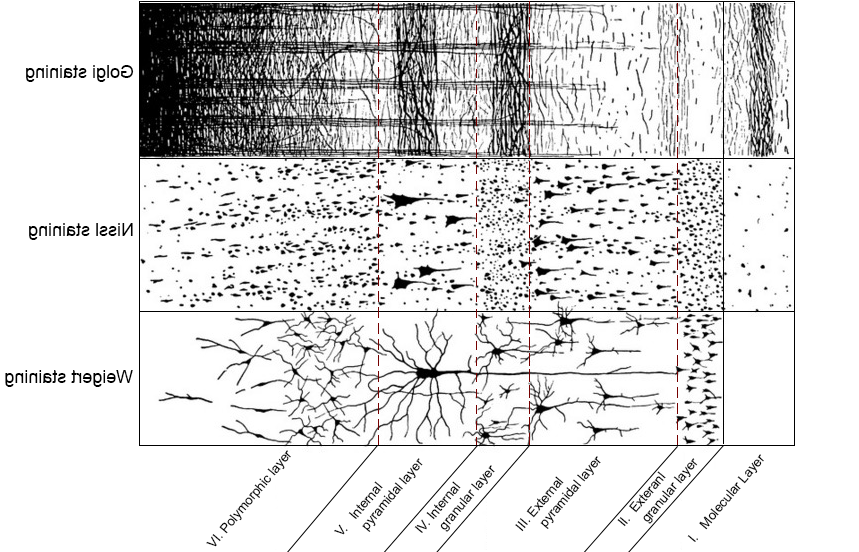
\includegraphics[width=0.8\textwidth, clip=true]{./Chapters/01_Introduction/Images/Layers}
	\caption{\cite{Brodman1909} }
	\label{fig:layers}
\end{figure}

For a small set of experiments, it is relatively straightforward to say if they are feed forward or feedback, but now think of more complicated processes: what would constitute as feed forward in language processing, decision making or memory? This is largely unknown and that is why it is of great interest to learn more about the laminar processing. It could shed light on a multitude of cognitive processes and open doors to a whole new type of information and new research in the brain \cite{Lawrence2017}. However, the greatest barrier is that is neuronal communication is not easily measured. With fMRI, only a derivative of neuronal firing can be measured as changes in oxygen consumption. We will therefore first need to get a better understanding of what type of information it is that fMRI can yield.

\section{Contrast Mechanisms}
Neurons clearly have layer specific functions, but measuring them is not easy, especially not in living humans. We cannot put electrodes in their heads, but what we can do is put them in an MRI scanner. An MRI scanner, however, cannot measure direct neuronal firing. Instead, it is susceptible to all kinds of magnetic properties of which three dimensional images can be made. Most notably, the magnetic susceptibility of red blood cells changes when they are oxygen rich or oxygen poor \cite{Ogawa1990}, which we call the Blood Oxygenation Level Dependant Signal, the BOLD signal. However, while there is little doubt that activation in a cortical region elicits a BOLD response, large parts of the biological mechanism behind it are still disputed. Most importantly, the extent to which the BOLD response reflects laminar specific activation is largely unknown. 

It was noted that maybe more so than just activity (MUA, multi unit acitvity), the amount of synaptic input (measured by the local field potential, LFP) migth be crucial for the strength of the BOLD response \cite{Goense2008}.

\begin{figure}[!ht]
	\centering
	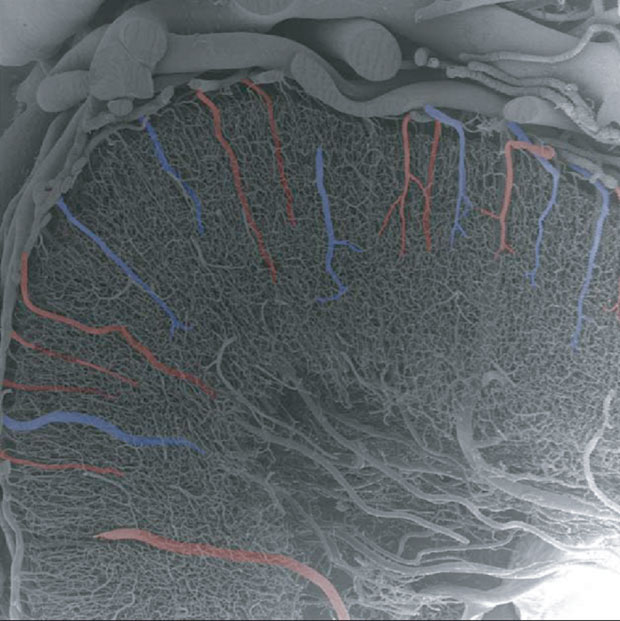
\includegraphics[width=0.9\textwidth, clip=true]{./Chapters/01_Introduction/Images/Microvasculature}
	\caption{The microvasculature of the visual cortex of a macaque \cite{Weber2008}. }
	\label{fig:microvasulature}
\end{figure}
Figure~\ref{fig:microvasulature} shows the microvasculature of a small piece of visual cortex in a macaque. In red, the arterioles, small blood vessels that dive from the top of the cortex (the pial surface) downward to supply the whole grey matter from blood. The smallest vessels, the capillaries, relay the oxygen to the neurons in all cortical layers, such that deoxygenated hemoglobin is drained away by the veins (blue). The veins on top of the cortex can be an order of magnitude larger than the cortical veins, and conduct off the deoxygenated blood. This might make one appreciate the difficulty of extracting laminar specific signals with large signals of non-interest in the direct neighbourhood. 

But the level of blood oxygenation is not the only quantity that fluctuates as a result of cortical activation. More blood starts flowing (higher cerebral blood flow, CBF), vessels start dilating (more cerebral blood volume, CBV) and the consumption of oxygen increases (higher cerebral metabolic rate of oxygen, CMR$_{O2}$). These quantitative measures can be related to one another by the Davis model, save some free parameters that need to be empirically determined \cite{Davis1997}. However, the proposed equations hold for the cortical column in its entirety, but does not take into account potential layer specific differences. 

So while we cannot measure neuronal activation with MRI, the closest we can get is the traces in the magnetic properties in the vasculature through BOLD, CBV, CBF, and CMRO$_{2}$. The extent to which these quantities vary as spatially specific as the level of the cortical layers is an outstanding question, however, and needs to empiraclly tested. Indeed, there are techniques to measure them, $T_2^*$-weighted imaging \cite{Norris2006} for BOLD, VASO for CBV \cite{Huber2018}, arterial spin labelling \cite{Grade2015} for CBV, and calibrated BOLD \cite{Blockley2013}) for CMRO$_{2}$. All vary in terms of sensitivity, specificity, and attainable resolution (spatial as well as temporal). The spatial resolution in combination with the type of experiment that is required for CBF and CMRO$_2$ measurements makes them poor candidates for human in vivo fMRI. It is mainly BOLD and CBV that have shown promising layer specific differences in animal experiments \cite{Lu2004,Zhao2006,Jin2008,Goense2012}. The main benefits of VASO compared to BOLD are its quantifiability \cite{Lu2003} and local specificity \cite{Jin2006}, whereas BOLD has higher sensitivity and speed \cite{Huber2018}.

Our main goal was to investigate the possibilities of laminar analysis in standard experiments on humans, and hence chose to use the BOLD signal as our signal of interest. Fundamentally, the BOLD signal arises as a consequence of magnetic field perturbations arising from desoxyhemoglobin molecules \cite{Norris2006}. These changes extend beyond the blood vessel and drop off as a function of field strength, the orientation of the vessel, and the vessel diameter. 
From the time that the molecules are excited until the time of the echo, molecules move around through the vessel. If the trajectory of a molecule in this time is small compared to the vessel size (and hence compared to the drop-off), there is little change in its surrounding magnetic field and the effect is reversible, a static effect. If on the other hand the molecule's trajectory is large, its surrounding magnetic field changes more drastically and unpredictably, such that the effect is irreversible and dynamic.
These two contrast mechanisms are the static and dynamic extravascular effect
The magnetic field perturbations scale linearly with field strength, so the trajectory of a molecule relative to the perturbations is much greater at 7 Tesla than at 1.5 Tesla. Thus, the dynamic extravascular effect increase with field strength. 
The remaining static effect at 7 Tesla is thus very specific, but detecting it requires high sensitivity \cite{Panchuelo2014}. 
An additional source of BOLD contrast is the intravascular effect. The magnetic field inside the vessel is slightly different from the surrounding tissue because of the amount of desoxyhemoglobin. As a result, the signal will start to dephase with respect to the extravascular signal. This is can be reversed because it is constant over time and is called the static intravascular effect. The exact origin of the last contrast mechanism is unclear. This is irreversible (dynamic) intravascular dephasing and has to do with the random movement of water molecules within red blood cells. It is either due to these water molecules interacting with the deoxyhemoglobin, or with the diffusion in and out of the cells, but no experiment to date has been able to tease the two mechanisms apart.
Four different contrast mechanisms can be distinguished.

Even given these four contrast mechanisms, it is still an outstanding question in what proportions they proliferate in measurements. This may even vary at the laminar level, as the deoxyhemoglobin from deeper layers flows upward to the top layers. The strengths of these effects have been modelled \cite{Markuerkiaga2016,Uludag2017} for both spin echo and gradient echo and suggest that most of the signal produced in a layer is also visible in that layer. For spin echo this is almost fully the case, while gradient echo has a tail that extents to more superficial layers, but at a gain of sensitivity. A range of laminar profiles has been found using spin echo (e.g. \cite{Zhao2004,Harel2006,Goense2006}), gradient echo (e.g. \cite{Polimeni2010,DeMartino2013,Chen2013}) or a combination of both, GRadient A Spin Echo (GRASE) \cite{Olman2012,DeMartino2013}.

Choosing a sequence requires carefully balancing the advantages and disadvantages against each other. We here chose to use gradient echo to investigate the laminar BOLD signal for its higher sensitivity at a field strength of 7 Tesla for high specificity. The potential downside of this is the susceptibility to the larger veins on top of the cortex that might obscure smaller effects \cite{Barth2007}. While the exact origins of the BOLD signal are unknown, there is strong evidence that the BOLD signal has a laminar footprint \cite{Logothetis2001}. Although some results from animal studies suggest that the effects may be visible at a higher temporal resolution than human in vivo MRI can achieve \cite{Yu2014,OHerron2016}. With the many uncertainties and the small size of the potential effect, it is soon clear that any potential effect can only be picked up with powerful methods that address as many sources of noise as possible. 

\subsection{Methods}
After covering the fundamentals of measurement techniques, it is clear what types of information may be expected to be present in the data. Getting out the relevant information, however, is at least as complicated. The brain is a highly convoluted structure that we are trying to describe and visualise by means of cubic voxel rasters. The first problem we encounter is a geometrical one: how do we attach a brain location to voxels in space? This can be done by making a \emph{cortical reconstruction} on a high resolution brain scan \cite{Dale1999,Bazin2012} with a very clear contrast between the white matter and grey matter as seen in Figure~\ref{fig:mybrain}. The distinction between white and grey matter is clear enough to draw a three dimensional boundary on both side of the grey matter: on the white matter boundary and one on the pial surface, the separation between the grey matter and the cerebrospinal fluid (CSF).
\begin{figure}[!ht]
	\centering
	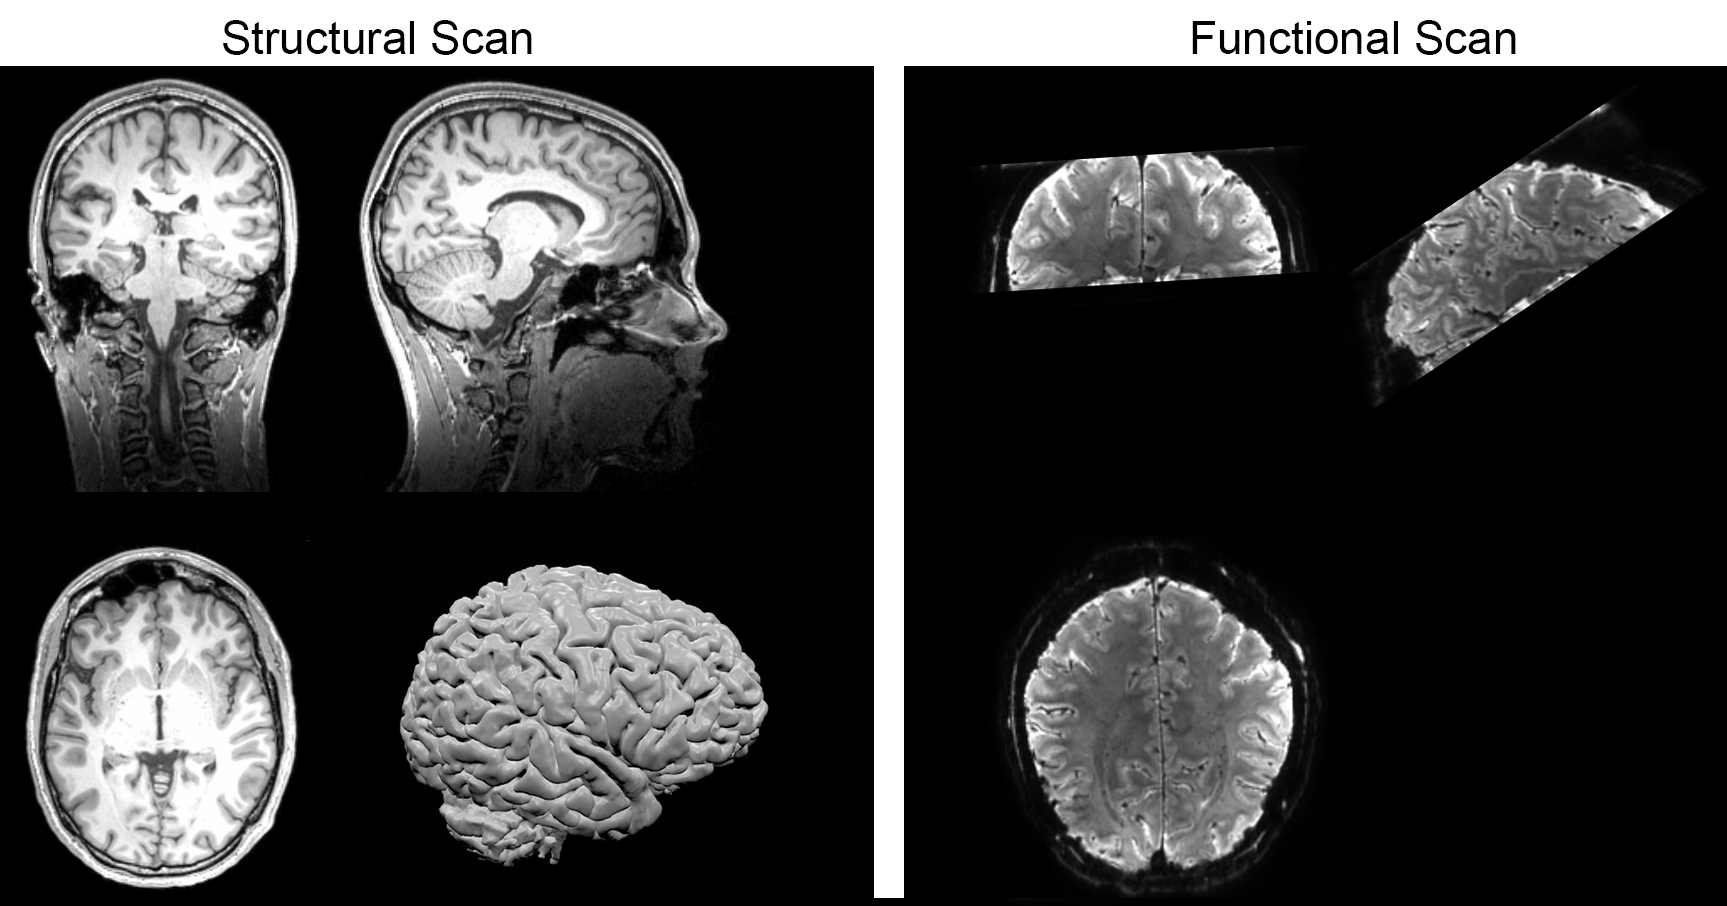
\includegraphics[width=0.99\textwidth, clip=true]{./Chapters/01_Introduction/Images/MyBrain}
	\caption{An example of a structural and functional brain scan. On the left, the structural scan has high anatomical contrast and sharp differences between the white matter and grey matter. The contrast is sharp enough to make a three dimensional reconstruction of the brain (lower right corner). On the right, a functional image is shown. The anatomical contrast is much weaker, but it can be acquired quickly and the contrast is susceptible to slight changes in blood deoxyhemoglobin, related to oxygen consumption on neuronal activation.}
	\label{fig:mybrain}
\end{figure}

The cortical reconstruction is very informative about the shape of the brain and potentially also about the layers: One could imagine different layers to be described as intermediate surfaces between both outer boundaries of which the locations can be used to then sample the cortical layers \cite{Koopmans2011,Polimeni2010,DeMartino2013}.
This descriptions allows for all sorts of surface base calculations \cite{Fischl2000,Bazin2012} and for example allows us to take into account a more naturalistic flow of the cortical layers \cite{Bok1929,Waehnertr2014}. Here it is described 



The people that we scan will move, breathe, fall asleep, ca
The scanner 


When we talk about a scanner with a field strength of 7 Tesla, it means there should be a homogeneous static magnetic field of that strength in the centre of the scanner. However, because the presence of a human body perturbs the field, it is not as homogeneous as one might want. Small perturbations can be corrected by \emph{shimming}, applying an additional magnetic field to compensate for the inhomogeneities. However, this is not accurate enough to correct all deviations and the inhomogeneities need not be constant over time. 


Distortion. The magnetic field is not always homogeneous



Multiple types 


It is possible geometrical properties 


%%
Balloon model \cite{Buxton1998}
something with a dynamic model of the hemodynamic signal \cite{Friston2000}.
















\section*{Thesis outline}
This thesis covers two major problems in laminar fMRI that needed to be solved before an experimental study could be conducted, and will reflect on building an fMRI pipeline, laminar or otherwise. In Chapter~\ref{ch:registration}, we will discuss a new way of coregistering an anatomical scan with a functional scan, when the latter is non-linearly distorted. We explain the details of the distortion correction technique, show its performance, and freely provide the code and data online. Chapter~\ref{ch:glm} describes a novel way of extracting laminar signal from data. We show its performance on a multitude of data, from a simulated fMRI model to post mortem data, to in vivo data from a set of subjects. Having overcome several of the most challenging aspects of laminar analysis, we then proceed to a laminar experiment in Chapter~\ref{ch:attention}. In a visual attention experiment, we investigate the laminar response. We further developped a new tool to more easily build fMRI analysis pipeline, to more reprodicibly conduct science, and to easily share analysis pipelines with others in Chapter~\ref{ch:porcupine}. Finally, these results will be put in a broader perspective in the Discussion, Chapter~\ref{ch:discussion}.


\linespread{1.5}
\newpage

%\linenumbers
\afterpage{\blankpage}
\chapter{Preserved Spontaneous Mentalizing amid Reduced Intersubject Variability in Autism during a Movie Narrative}
\label{ch:mentalizing_asc}

\begin{center}
    \large\textit{Abstract}
\end{center} 

{\abstractfont 
While individuals with autism often face challenges in everyday social interactions, they may demonstrate proficiency in structured mentalizing tasks that assess their ability to infer others' mental states. Using functional MRI and pupillometry, we investigated whether these discrepancies stem from diminished spontaneous mentalizing or broader difficulties in unstructured contexts. Fifty-two adults diagnosed with autism and 52 neurotypical controls viewed 'Partly Cloudy', a nonverbal animated film with a dynamic social narrative known to engage the mentalizing brain network during specific scenes. Analysis focused on comparing brain and pupil responses to these mentalizing events. Additionally, dynamic intersubject correlations explored the variability of these responses throughout the film. Both groups showed similar brain and pupil responses to mentalizing events and provided comparable descriptions of the characters' mental states. However, participants with autism exhibited significantly stronger correlations in their responses across the film's social narrative, indicating reduced inter-individual variability. This distinct pattern emerged well before any mentalizing events and involved brain regions beyond the mentalizing network. Our findings provide functional evidence of spontaneous mentalizing in autism, demonstrating this capacity in a context affording but not requiring mentalizing. Rather than responses to mentalizing events, a novel neurocognitive signature - inter-individual variability in brain and pupil responses to evolving social narratives - differentiated neurotypical individuals from those with autism. These results suggest that idiosyncratic narrative processing in unstructured settings, a common element of everyday social interactions, may offer a more sensitive scenario for understanding the autistic mind. \par
} 

\vspace*{\fill} 
This chapter is adapted from: \bibentry{mangnus2024bpcnni}

\thispagestyle{empty}

\newpage

\section{Introduction}
Autism Spectrum Condition (ASC) is a neurodevelopmental disorder marked by difficulties in social communication and interaction across multiple contexts \citep{apa2013}. These difficulties are frequently associated with mentalizing - the ability to attribute mental states to oneself and others \citep{premack1978,wimmer1983}. While initial findings suggested diminished mentalizing abilities in autism \citep{baron-cohen1985,happe1994}, subsequent studies have painted a more complex picture, owing to a variety of factors.

First, the reliability of established mentalizing assessments, such as the False Belief Test, Strange Stories, and the Reading the Mind in the Eyes Test, has increasingly come under scrutiny. These tests have shown inconsistent effect sizes when compared to earlier, smaller-scale studies and exhibit limited correlations with one another, despite their aim to measure similar or identical mentalizing constructs \citep{gernsbacher2019,higgins2024,schaafsma2015,yeung2024}. Second, many studies do not adequately match autistic individuals with neurotypical controls based on language abilities, which are crucial to varying degrees for these tasks \citep{betz2019}. This lack in language matching is particularly significant given the generally lower performance in verbal learning and memory observed within the autism population \citep{velikonja2019}. Lastly, recent research highlights the remarkable proficiency of autistic individuals in mentalizing tasks, especially in situations requiring strategic mental state reasoning \citep{bowler1992,pantelis2017}, such as deception \citep{vantiel2021}.

Faced with these empirical challenges, researchers have turned to more implicit mentalizing measures. This includes the analysis of anticipatory eye movements concerning an actor's false beliefs \citep{senju2009}, and measuring neural activity in the Animated Triangles task, where participants attribute mental states to moving shapes \citep{abell2000}. Recent findings indicate that while autistic individuals do show anticipatory gaze responses, these responses tend to be generally slower, regardless of whether the character's beliefs were true or false \citep{glenwright2021,schuwerk2016}. In the Animated Triangles task, both autistic and neurotypical participants show comparable brain activation in key mentalizing regions, such as the medial prefrontal cortex (mPFC), temporoparietal junction (TPJ), and precuneus \citep{moessnang2020}. However, individuals with autism typically underperform in both the mentalizing and non-mentalizing conditions of this task, which, combined with their generally slower anticipatory gaze responses, points to broader difficulties in implicit task settings \citep{wilson2021}. The extent to which autistic individuals engage in spontaneous mentalizing, particularly in unstructured settings lacking an explicitly defined task, as is common in everyday social interactions, remains largely unknown.

In this study combining fMRI and pupillometry, we aimed to bridge this knowledge gap by investigating how individuals with and without autism respond to mental state events embedded in a dynamic movie narrative. Additionally, we sought to provide insights into how these individuals process stimuli in less structured environments that more closely resemble everyday social interactions. Everyday interactions require a continuous assessment of stimuli within an evolving narrative \citep{goffman1974,johnson2023,stolk2022}, as seen in how even seemingly minor behaviors like a voluntary cough or a brief silence can carry significant implications in certain contexts \citep{kendon1994}. Failure to recognize these narrative cues could lead to misunderstandings in scenarios that require high levels of interpretation, such as irony or sarcasm, areas known to pose challenges for autistic individuals \citep{deliens2018,zalla2014}. However, capturing this narrative processing is challenging, as it likely unfolds differently over time among individuals exposed to the same stimuli. We reasoned that narrative processing could manifest as inter-individual variability in responses to movie stimuli, particularly diminished among those less inclined to interpret stimuli through a narrative lens \citep{chang2021,finn2018,owen2023,zhang2022}. We investigated this possibility using intersubject correlation analysis \citep{hasson2004}, applying it to two complementary methods for assessing cognitive processing: brain imaging and measurements of pupil size \citep{beatty1982}. 

To probe spontaneous mentalizing and narrative processing, we recorded participants' brain and pupil responses as they viewed the nonverbal animated movie `Partly Cloudy'\citep{jacoby2016,paunov2019}. Although movies cannot fully replicate the complexities of real-world social interactions \citep{wheatley2019}, they offer an effective platform for immersing participants in an evolving narrative under uniform stimulus conditions. To assess differences in narrative processing between autistic and neurotypical participants at various points during the movie, we augmented our intersubject correlation analysis with a dynamic sliding window technique and an adaptive clustering algorithm \citep{maris2007}. The movie Partly Cloudy was chosen for its proven ability to evoke neural activations within the mentalizing network through distinct mental state events \citep{jacoby2016,richardson2018}, making it suitable for evaluating spontaneous mentalizing. After viewing, we analyzed participants' verbal descriptions of the movie, focusing on their use of language related to mental states. This experimental approach enabled us to simultaneously probe spontaneous mentalizing and narrative processing, providing insights into how these cognitive functions interact in individuals with autism.

\section{Materials and methods}
\subsection{Preregistration and Data availability}
The study comprised two sets of preregistered analyses \citep{mangnus2022}. The first set focused on spontaneous pupil and brain responses to movie events anticipated to elicit mental state inferences, complemented by a questionnaire that examined participants' use of related vocabulary in describing the movie. The second set of analyses explored dynamic intersubject correlations to investigate idiosyncratic narrative processing throughout the entire movie. Unlike the event-related analyses, these exploratory analyses were not limited to specific movie segments. All resulting pupillometry and fMRI data are publicly available for further research \citep{mangnus2024dataset}. 

\subsection{Participants} 
The study enrolled 104 participants, divided equally into 52 adults diagnosed with Autism Spectrum Disorder (ASC) and 52 neurotypical controls (NT). Recruitment occurred through Radboud University's database, social media, campus postings, and outpatient clinics in Nijmegen and Arnhem, the Netherlands. Eligibility for the ASC group required a formal diagnosis from a clinician \citep{apa2013}, while exclusion criteria for all included the use of psychotropic drugs, severe cognitive impairment, systemic diseases, or neurological treatment history. As shown in Table~\ref{tab:ppt-stats-asc}, both groups were demographically matched for gender, age (Kullback-Leibler divergence = .05, \textit{F}-test (102) = .29), and both verbal and nonverbal IQ, verified through the Similarities and Vocabulary subscales of the Wechsler Adult Intelligence Scale (WAIS-III \citep{wechsler1997}; KL = .02, \textit{F}-test = .74) and Raven's Progressive Matrices (RPM \citep{raven1989}; KL = .01, \textit{F}-test (102) = .63). ASC participants notably scored higher on the Autism-Spectrum Quotient (AQ-50 \citep{baron-cohen2001AQ}), confirming group distinctions. Data collection involved MRI scans (\textit{n} = 104) and pupillometry (\textit{n} = 100) while participants viewed the film, followed by a post-viewing questionnaire completed by most (\textit{n} = 101). All participants provided written informed consent, approved by the local ethics committee (CMO region Arnhem-Nijmegen, file number 2019-6059), and received compensation for participation.

\begin{table}[ht]
    \captionsetup{justification=raggedright, singlelinecheck=false, font = normal} % Left-align the caption
    \caption{Demographic data}
    \label{tab:ppt-stats-asc}
    \setlength{\tabcolsep}{10pt}
    \renewcommand{\arraystretch}{1.5} % Adjust row spacing (default is 1.0)
    \begin{tabular}{llll}
    \hline
    \textbf{} & \textit{ASC Group} & \textit{NT Group} & \textit{Group Difference} \\
    \hline
    N (men:women) & 52 (23:29) & 52 (20:32) & \textit{$\chi$\textsuperscript{2}}(1, \textit{N} = 104) = 1.73, \textit{p} = .19 \\
    Age (years) & 27.7 (6.3) & 25.9 (5.5) & \textit{t}(102) = 1.74, \textit{p} = .08 \\
    Verbal IQ (WAIS-III) & 126 (16) & 124 (16) & \textit{t}(102) = 0.51, \textit{p} = .61 \\
    Nonverbal IQ (RPM) & 103 (9) & 104 (11) & \textit{t}(102) = -0.46, \textit{p} = .64 \\
    Autism Quotient & 31 (9) & 12 (6) & \textit{t}(102) = 12.2, \textit{p} < .001 \\
    \hline
    \multicolumn{4}{l}{\small{Values are given as Mean (Standard Deviation). ASC, Autism Spectrum Condition; NT, Neurotypical.}} \\
    \end{tabular}
\end{table}
    

\subsection{Experimental design }
Participants watched the 5-minute and 45-second animated short Partly Cloudy, depicting the evolving friendship between a stork and a cloud through various social interactions integral to its narrative. After viewing, they described the plot to assess narrative comprehension and articulation of characters' mental states. Descriptions were analyzed by independent raters, categorizing words into mental state terms or other content-related categories, using the mental state word list from \cite{bang2013}. An independent \textit{t}-test compared the frequency of mental state words used between groups. The movie featured three types of events, coded by the original research team that introduced it as a mentalizing localizer task \citep{jacoby2016}. These included \textit{Mental}, \textit{Pain}, and \textit{Control} events, each annotated on the movie's timeline in Fig~\ref{fig:task-fig-asc}. \textit{Mental} events, totaling 44 seconds across 4 events, were expected to elicit inferences about characters' mental states, depicting scenarios like characters feeling distressed while observing others enjoy a cheerful interaction or mistakenly perceiving betrayal by a friend. \textit{Pain} events, totaling 26 seconds across 7 events, depicted instances where characters experienced physical discomfort, such as being shocked by an eel or bitten by a crocodile. \textit{Control} events, totaling 24 seconds across 3 events, showcased serene moments like birds in flights or panoramic views of clouds. As detailed in later sections, these categorizations facilitated the analysis of mentalizing-related pupillary and neural responses.

\begin{figure}[!ht]
	\centering
    \makebox[\textwidth][c]{\includegraphics[width=1.05\textwidth]{./Chapters/02_MentalizingASC/Images/TaskFig.eps}}
	\caption{Autistic and neurotypical participants viewed a six-minute animated movie portraying the evolving friendship between a stork and a cloud, while their pupil and brain responses were recorded. Originally used by Jacoby et al. (2016) as a Theory of Mind localizer, the movie includes three types of events: Mental, Pain and Control, each marked on the movie timeline. Mental and Pain events were expected to prompt inferences about characters' mental and physical states, whereas Control events featured no characters in the foreground. The event images shown were generated using Copilot in Bing for copyright purposes to closely resemble scenes from the movie.}
    \vspace*{-10pt}
	\label{fig:task-fig}
\end{figure}

%[width=.9\textwidth]



\subsection{Pupillometry and MRI data acquisition}
Pupil size was continuously tracked using an Eyelink 1000 plus eyetracker at 1000 Hz. MRI data were acquired using a Siemens 3T MRI-scanner with a 32-channel head coil. Structural images were obtained with a T1 MPRAGE sequence (TR = 2200 ms, TI = 1100 ms, TE = 2.6 ms, flip angle = 11\textdegree, 
voxel size = 0.8 mm\textsuperscript{3}, acceleration factor = 2). Functional images were acquired with a multi-band multi-echo sequence (TR = 1500 ms, TE = 13.4/34.8/56.2 ms, flip angle = 75\textdegree, voxel size = 2.5 mm\textsuperscript{3}, acceleration factor = 2). Analysis of head movement through framewise displacement (FD) showed no significant differences between the ASC and NT groups. Mean FD was 0.15 \textpm{}{} 0.05 for ASC and 0.16 \textpm{}{} 0.09 for NT (M \textpm{} SD; \textit{t}(102) = -0.78, \textit{p} = .43), with maximum FD values at 0.81 \textpm{} 0.79 for ASC and 1.03 \textpm{} 1.31 for NT (\textit{t}(102) = -1.09, \textit{p} = .28). Additionally, assessments of total head motion, calculated from translation and rotation during the realignment process, indicated no significant differences (Translation: 109.5 \textpm{} 74.6 vs. 114.3 \textpm{} 99.5, \textit{t}(102) = 0.28, \textit{p} = .78; Rotation: 2.0 \textpm{} 0.98 vs. 2.2 \textpm{} 1.2 , \textit{t}(102) = 0.74, \textit{p} = .46).

\subsection{Pupillometry data analysis}
Pupillometry data underwent preprocessing with a combination of established and custom MATLAB routines. Blinks were removed using a noise-based detection algorithm \citep{hershman2018}. Squints, marked by unusually small pupil sizes \citep{mathot2018}, and gaze jumps, indicative of excessive translational eye movements, were both identified and eliminated through visual inspection. After these adjustments, 89.3\% \textpm{} 9.4\% of the data remained usable for the ASC group and 88.4\% \textpm{} 10.6\% for the NT group (\textit{t}(98) = 0.48, \textit{p} = .63). Fixations and saccades were distinguished using an adaptive velocity threshold \citep{nystrom2010}. Pupil timeseries were normalized (\textit{z}-scored) and adjusted for global luminance fluctuations modeled using the \textit{lm()} function from the R \textit{stats} package \citep{bates2015} up to the 5th polynomial order, validated with data from five randomly selected participants. Luminance was quantified using RGB values based on the Rec. 709 formula \citep{itu2002}. 

Event-related pupil responses were analyzed through a 3x2 mixed-design ANOVA with mean pupil size as the dependent variable, and event conditions (\textit{Mental, Pain, Control}) and participant group status (ASC, NT) as factors. Tukey's Honest Significant Difference tests further investigated mentalizing-related contrasts, specifically comparing \textit{Mental} to both \textit{Pain} and \textit{Control} conditions. To verify the robustness of our findings against variations in event timing, a control analysis was conducted by incorporating an additional time-based regressor into the \textit{lm()} function during preprocessing. This adjustment, which incremented by one every second, did not influence the main findings.

Intersubject variability was assessed using dynamic intersubject correlation analysis of the pupil timeseries. Employing a leave-one-out approach, each participant's timeseries was correlated with the composite average timeseries of all other group members \citep{nastase2019}. This analysis was conducted using a 30-second sliding window at 100 ms intervals, generating a correlation timeseries for the entire movie duration per participant. All correlation timeseries were Fisher \textit{z}-transformed and subjected to a nonparametric cluster-based permutation test \citep{maris2007}. This test addresses the multiple comparisons problem in timeseries analysis by clustering significant neighboring data points. These clusters are tested against a null distribution formed by randomly shuffling participant labels and recalculating statistics, allowing the identification of specific timepoints where significant differences in pupil response variability between groups occurred, while effectively controlling for false positives. Statistical testing was performed using a two-sided independent samples \textit{t}-test with 10,000 permutations to establish the null distribution. Clusters that reached a Monte-Carlo \textit{p}-value of .05 or less were considered statistically significant.

\subsection{fMRI data analysis}
Functional images were preprocessed using SPM12, initially consolidating multiple echoes into single volumes through echo-weighted combinations. These volumes were realigned to the initial image using rigid-body transformations and 2nd degree B-spline interpolation, and subsequently unwarped with participant-specific fieldmaps to minimize spatial distortions and signal dropout. Anatomical images were coregistered to the mean functional image and segmented into gray matter, white matter, and cerebral spinal fluid categories using SPM's tissue probability maps, enabling normalization to MNI space. An 8 mm full-width at half-maximum kernel was applied or spatial smoothing. First-level regressors estimated activations for \textit{Mental, Pain,} and \textit{Control} events, and included adjustments for head movement (using squared and cubic terms, along with first and second derivatives) and tissue signal intensities. A 0.6 threshold masking was applied to ensure optimal brain coverage.

Two 2-by-2 mixed-design ANOVAs were conducted to analyze mentalizing activations across \textit{Mental, Pain,} and \textit{Control} conditions and participant groups (ASC, NT). The first contrast (\textit{Mental} > \textit{Pain}) sought to confirm previous findings of enhanced mentalizing network activity \citep{jacoby2016}, while the second (\textit{Mental} > \textit{Control}) extended these findings to scenes lacking foreground characters. Results were subjected to whole-brain, cluster-level correction (\textit{p\textsubscript{FWE}} < .05), with anatomical locations identified using the SPM Anatomy Toolbox \citep{eickhoff2005}. Additionally, a region of interest (ROI) analysis focused on three peak brain regions, complemented by Bayesian analysis \citep{jasp2022} to evaluate consistent neural activation within the mentalizing network across groups, reporting evidence with Bayes Factors (BFs). Robustness against event timing variations was confirmed through a control analysis adding a first-level regressor that incremented with each volume.

Intersubject variability at the neural level was assessed using dynamic intersubject correlation analysis of voxel timeseries, adjusted for head movement and tissue signals. Mirroring the pupillometry analysis, a leave-one-out and sliding window method generated whole-brain correlation timeseries for each participant. For computational efficiency, the data were spatially and temporally downsampled by a factor of three, resulting in a voxel resolution of 7.5 mm and a sampling interval of 4.5 seconds. These data underwent a nonparametric cluster-based permutation test \citep{maris2007}, which corrected for multiple comparisons across voxels and timepoints using a two-sided independent samples \textit{t}-test with 10,000 permutations (Monte-Carlo \textit{p} < .05). The analysis was further refined with a spatially adaptive clustering algorithm, identifying variations in brain response patterns between groups. The spatial distribution of the identified spatiotemporal brain cluster was visualized by summing t-values across all timepoints, producing a three-dimensional representation of significant variability. The degree of overlap between this cluster and the mentalizing network was quantified by comparing their spatial volumes. Lastly, a supplementary analysis without the sliding window approach calculated correlations across the entire voxel timeseries, pinpointing a smaller cluster in the left supramarginal gyrus. In line with the main findings, this cluster demonstrated reduced intersubject variability in the ASC group.

\section{Results}
\subsection{Post-viewing movie descriptions }
After the film viewing, participants were asked to recount the story of the stork and cloud's evolving friendship in their own words. We analyzed these descriptions for the use of mental state words and other content-related terms (Fig~\ref{fig:beh-pupil-asc}a). Statistical analysis revealed no significant differences in the frequency of mental state word usage between the autistic and neurotypical participants (M\textsubscript{ASC} = 0.063, M\textsubscript{NT} = 0.054, \textit{t}(99) = 0.84, \textit{p} = .40; Fig. 2b), with a Bayes Factor in favor of the null hypothesis (BF\textsubscript{Null} = 3.49). This finding suggests that both autistic and neurotypical groups engaged similarly with the mental states depicted in the film.

\begin{figure}[!ht]
    \vspace*{10pt}
	\centering
    \makebox[\textwidth][c]{\includegraphics[width=1.05\textwidth]{./Chapters/02_MentalizingASC/Images/BehPupil.eps}}
	\caption{Comparable mental state descriptions and pupil responses across groups. (a) Word Cloud depicting the frequency of mental state-related vocabulary used by participants in their post-viewing movie descriptions. The size of each word corresponds to its frequency of use. (b) Bar graphs displaying the ratio of mental state words to other content-related terms in these descriptions, showing no significant differences between the two groups. (c) Pupil responses across all event conditions, revealing similar response patterns in both autistic and neurotypical groups. Asterisks denote significant differences between event conditions (all \textit{p} < .001), with no significant differences observed between groups. Outliers are represented by dots, while whiskers display a 1.5 inter-quartile range.}
    \vspace*{-10pt}
	\label{fig:beh-pupil-asc}
\end{figure}



\subsection{Event-related pupil responses}
Participants' pupil sizes were continuously tracked throughout the movie to assess responses to events expected to elicit mental state inferences, such as the cloud reflecting on the stork's actions. We also analyzed responses to events evoking physical state inferences, like the stork experiencing pain, as well as to control scenes devoid of character interactions. Pupillometry analysis identified distinct responses to these three event types (\textit{F}(2,196) = 73.0, \textit{p} < .001, BF\textsubscript{Null} = 0.00; Fig~\ref{fig:beh-pupil-asc}c), with the largest pupil dilation occurring during \textit{Pain} events (M = 0.22, \textit{z}-score), followed by \textit{Mental} events (M = -0.12) and \textit{Control} events (M = -0.20). Comparisons of pupil responses between autistic and neurotypical participants revealed no significant differences (\textit{F}(1,98) = 0.03, \textit{p} = .86, BF\textsubscript{Null} = 7.8), nor were there significant interaction effects between participant groups and event types (\textit{F}(2,196) = 2.1, \textit{p} = .12, BF\textsubscript{Null} = 2.5). This suggests that both groups reacted similarly to the different event types in the movie.

\subsection{Event-related brain responses}
A whole-brain fMRI analysis was conducted to examine neural activations during \textit{Mental} events in comparison to \textit{Control} and \textit{Pain} events. As depicted in Fig~\ref{fig:fmri-results-asc}a, this analysis identified robust activation in keys areas of the mentalizing network \citep{schurz2014}, specifically in the right and left temporoparietal junction (rTPJ: xyz\textsubscript{MNI} = [48, -62, 32], \textit{t} = 16.85, \textit{p\textsubscript{FWE}} < 0.001; lTPJ: [-46, -62, 32], \textit{t} = 16.92, \textit{p\textsubscript{FWE}} < 0.001), the precuneus ([6, -64, 40], \textit{t} = 20.64, \textit{p\textsubscript{FWE}} < 0.001), medial prefrontal cortex (mPFC: [-6, 52, 38], \textit{t} = 7.33, \textit{p\textsubscript{FWE}} < 0.001), and left middle temporal gyrus ([-52, 2, -26], \textit{t} = 11.51, \textit{p\textsubscript{FWE}} < 0.001). Echoing the pupillometry findings, no significant differences in neural activation were observed between autistic and neurotypical participants. Complementary region of interest (ROI) analyses (Fig~\ref{fig:fmri-results-asc}b) and Bayesian analyses reinforced these findings, providing evidence favoring the null hypothesis over alternative models suggesting group differences. This was consistently demonstrated across all evaluated ROIs for both \textit{Mental} > \textit{Pain} contrasts (rTPJ: BF\textsubscript{Null} = 4.83, precuneus: BF\textsubscript{Null} = 1.73, mPFC: BF\textsubscript{Null} = 4.01) and \textit{Mental} > \textit{Control} contrasts (rTPJ: BF\textsubscript{Null} = 3.43, precuneus: BF\textsubscript{Null} = 3.63,  mPFC: BF\textsubscript{Null} = 4.71), underscoring a similarity in neural processing of mental states among autistic and neurotypical individuals.

\begin{figure}[!ht]
	\centering
    \includegraphics[width=1\textwidth,trim={0 9cm 0 0},clip=true]{./Chapters/02_MentalizingASC/Images/FMRIResults.eps}
	\caption{Comparable neural activation patterns during mental state events across groups. (a) Brain sections showing whole-brain responses specific to mental state events, as assessed through the Mental > Control and Mental > Pain contrasts. There were no significant differences in activation for either contrast between the autistic and neurotypical groups. (b) Box plots depicting the contrast estimates for the Mental > Control (in blue) and Mental > Pain (in red) comparisons across various Regions of Interest (ROI) for both groups. rTPJ and mPFC were selected as ROIs based on mentalizing literature, while the precuneus was selected because of the peak voxel being located in that region for both mentalizing contrasts. Across all ROIs and contrasts, no significant differences were observed between the groups. Outliers are represented by dots, while whiskers display a 1.5 inter-quartile range.}
    \vspace*{-10pt}
	\label{fig:fmri-results}
\end{figure}

%\makebox[\textwidth][c]{



\subsection{Movie-driven variability in pupil responses }
Having observed comparable pupil and brain responses to mental state events and similar verbal descriptions from both autistic and neurotypical participants, we expanded our investigation to narrative processing differences across the entire movie through dynamic intersubject correlation analysis of the pupil timeseries. This analysis revealed an interval from 40 to 71 seconds where individuals with autism demonstrated significantly stronger correlations in pupil responses, indicating reduced intersubject variability compared to neurotypical participants (M\textsubscript{ASC} = 0.61, M\textsubscript{NT} = 0.55, \textit{cluster stat} = 777, \textit{p} = .045; Fig~\ref{fig:isc-pupil-asc}). This interval preceded any mental state events and coincided with scenes featuring storks flying through the air and clouds morphing into baby animals. Although this reduced variability continued throughout the film, it did not reach statistical significance outside this interval after adjusting for multiple comparisons. Further, differences in variability were not due to variations in saccadic eye movements, as their frequency and variability remained consistent between groups (Fig~\ref{fig:saccades-suppl}).

\begin{figure}[!ht]
    \vspace*{5pt}
	\centering
    \includegraphics[width=1\textwidth,clip=true]{./Chapters/02_MentalizingASC/Images/ISCPupil.eps}
	\caption{Reduced pupil response variability in autistic participants. Dynamic intersubject correlation analysis initially showed comparably high levels of correlation in both autistic and neurotypical groups at the start of the movie. However, a significant divergence emerged around the 40-second mark, where autistic individuals showed stronger correlations in their pupil responses, indicating reduced intersubject variability, compared to neurotypical participants. This pattern of reduced variability emerged well before the mental state events highlighted in red. Solid lines delineate statistically significant intervals, as determined by a cluster-based permutation test.}
    \vspace*{-15pt}
	\label{fig:isc-pupil-asc}
\end{figure}





\subsection{Movie-driven variability in brain responses}
When applied to the fMRI data, dynamic intersubject correlation analysis identified a spatiotemporal cluster where individuals with autism showed significantly stronger correlations in their brain responses compared to neurotypical participants (Fig~\ref{fig:isc-fmri-time-asc}). This cluster spanned the entire movie (\textit{cluster stat} = 1332, \textit{p} = .002) and included peaks in the right and left supramarginal gyrus (rSMG: xyz\textsubscript{MNI} = [52, -34, 32], \textit{t\textsubscript{max}} = 3.88; lSMG: [-54, -40, 32], \textit{t\textsubscript{max}} = 4.54), the right inferior temporal gyrus (rITG: [54, -22, -28], \textit{t\textsubscript{max}} = 5.90), and the left calcarine gyrus (lCG: [6, -102, -10], \textit{t\textsubscript{max}} = 4.20). The reduced variability was consistent across these regions for most of the movie (Fig~\ref{fig:isc-fmri-peak-suppl}), and it emerged well before and continued after any mental state events. The cluster's overlap with the mentalizing network was minimal, comprising less than 20\% of the total cluster size (Fig~\ref{fig:isc-fmri-overlap-asc}). This indicates that the observed reduced variability in brain responses among autistic participants extends beyond regions involved in mental state processing, suggesting broader differences in neural processing between the groups.

\begin{figure}[!ht]
	\centering
    \makebox[\textwidth][c]{\includegraphics[width=1.05\textwidth,clip=true]{./Chapters/02_MentalizingASC/Images/ISCFMRITime.eps}}
	\caption{Reduced brain response variability in autistic participants. Dynamic intersubject correlation analysis identified a spatiotemporal brain cluster where autistic individuals demonstrated significantly stronger correlations in their brain responses, indicating reduced intersubject variability, compared to neurotypical participants. This cluster persisted throughout the movie and featured peaks in the right and left supramarginal gyrus, the right inferior temporal gyrus, and the left calcarine gyrus. Echoing the pupillometry data, this pattern of reduced variability in autistic participants emerged well before the mental state events highlighted in red. LH, left hemisphere; RH, right hemisphere.}
    \vspace*{-10pt}
	\label{fig:isc-fmri-time-asc}
\end{figure}





\vspace*{.1cm}

\begin{figure}[!ht]
	\centering
    \includegraphics[width=1\textwidth,clip=true]{./Chapters/02_MentalizingASC/Images/ISCFMRIOverlap.eps}
	\caption{Limited spatial overlap between brain regions showing reduced intersubject variability in autistic participants and mentalizing activation. The overlap comprised less than 20\% of the total cluster size. For clarity, the cluster is visualized using a cumulative \textit{t}-value threshold of 20 or higher. Lateral brain images provide an overlay with a search distance of 10 mm. }
    \vspace*{-10pt}
	\label{fig:isc-fmri-overlap}
\end{figure}





\section{Discussion}
Using fMRI and pupillometry, this study provides functional evidence of spontaneous mentalizing abilities in individuals with autism. Compared to neurotypical controls matched for gender, age, and both verbal and nonverbal IQ, individuals with autism exhibited similar brain and pupil responses during movie scenes known to activate the mentalizing network \citep{jacoby2016,richardson2018}. Activity in the mentalizing network was enhanced during scenes that encouraged viewers to contemplate the actions and mental states of depicted characters. Conversely, scenes prompting physical state inferences, such as characters experiencing physical discomfort, or control scenes lacking central characters, resulted in weaker mentalizing activations. Verbal descriptions provided by participants after the movie corroborated these findings, indicating an engagement with the mental state events depicted in the movie on par with that of neurotypical controls. These results extend prior evidence of preserved mentalizing in autism \citep{moessnang2020,dufour2013}, showcasing this capacity in a situation affording but not requiring mentalizing.

While individuals with and without ASC showed comparable brain and pupil responses during mental state events, dynamic intersubject correlation analysis revealed significant differences in the correlation of these responses over extended movie intervals. Participants with autism exhibited significantly stronger correlations, indicating reduced inter-individual variability, across several brain regions outside the mentalizing network. These regions included the right and left supramarginal gyrus, linked to empathic judgment \citep{silani2013,wada2021}, the right inferior temporal gyrus, associated with narrative comprehension \citep{youssofzadeh2022}, and the left calcarine gyrus, crucial for visual processing \citep{woldorff2002}. This reduced variability was not due to differences in bottom-up processing, as both autistic and neurotypical groups exhibited similar saccadic eye movement patterns throughout the film. The most pronounced differences emerged during early scenes featuring storks flying through the air and clouds morphing into baby animals, which likely introduced significant narrative ambiguity. This ambiguity may have prompted neurotypical viewers to idiosyncratically interpret how these visual elements fit into the evolving storyline, resulting in less consistent responses. In contrast, autistic participants' responses appeared to be more consistently aligned with the movie's stimuli, possibly reflecting a heightened focus on specific details rather than the broader narrative context \citep{losh2003,tager-flusberg1995,barnes2012,geelhand2020,koldewyn2014}. Importantly, these differences manifested in cognitive and neural processing rather than in eye movements, suggesting that the variability observed in neurotypical responses may represent a neurocognitive signature of top-down processing.

The neuroanatomical bases of the observed changes in response variability are in line with existing research on autism and social interaction. Prior studies have documented structural alterations in the gray matter of both the right and left supramarginal gyrus in individuals with autism \citep{brieber2007,ke2008,libero2014}, as well as reduced anatomical connectivity in the right inferior temporal cortex \citep{boets2018,koldewyn2014}. This region exhibits prolonged activations during tasks involving story comprehension and interactive communication \citep{youssofzadeh2022,stolk2013neural}, highlighting its role in integrating stimuli within an evolving narrative. This integration is crucial for complex social interactions, which necessitate the continuous assessment of diverse stimuli to maintain narrative coherence with others \citep{goffman1974,johnson2023,stolk2022}. A key direction for future research is to examine how response variability in the identified brain regions differs across various social contexts. Such investigations will not only help to illuminate the specific challenges faced by autistic individuals in everyday social situations, but could also inform the development of interventions by identifying environments that promote effective social interaction \citep{wadge2019}.

It is worth noting that our intersubject correlation patterns differ from previous studies demonstrating greater brain response variability in autistic individuals compared to neurotypicals \citep{byrge2015,hahamy2015,hasson2009,lyons2020,nunes2019,ou2022,pegado2020,salmi2013}. Several factors could explain these discrepancies. First, our study used an animated film with fictional characters, as opposed to the more realistic human portrayals in other studies. Although the type of characters may influence brain responses in autism \citep{atherton2018}, greater neural variability has been noted with fictional characters \citep{lyons2020}. Second, we implemented an adaptive clustering algorithm to identify spatiotemporal clusters of brain response variability within 30-second intervals. This approach is potentially more sensitive to brain response variations associated with subtle shifts in interpretation than whole-movie analyses, which emphasize consistent patterns over significantly longer durations (10 to 67 minutes). This approach may more effectively capture the hypothesized increased reliance on bottom-up sensory stimulation in autism \citep{pellicano2012}, possibly leading to less variability in neural signals related to narrative interpretation. More generally, our findings invite a reconsideration of theories that propose precise neural synchronization as a means to manage individual perspectives in daily interactions \citep{holroyd2022}. These theories suggest that aligning neural responses to external cues helps individuals achieve a common viewpoint, thereby facilitating social interaction \citep{hasson2012,mayo2021}. However, contrary to expectations based on their social difficulties, participants with autism in our study displayed stronger neural correlations when exposed to the same external stimuli, challenging the assumed role of precise neural synchronization in social interaction \citep{stolk2014}.

In conclusion, this study offers functional evidence of spontaneous mentalizing in autism, showcasing this capacity in a context affording but not requiring mental state inferences. More distinctively, our findings identify a novel neurocognitive signature - inter-individual variability in brain and pupil responses to evolving social narratives - that differentiates neurotypical individuals from those with autism. These results underscore the importance of idiosyncratic narrative processing in unstructured settings, a hallmark of everyday social interactions, as a potentially more sensitive framework for understanding the autistic mind.
\newpage  
\section{Supplementary information} 

% table S1. 
\begin{table}[ht]
    \centering
    \captionsetup{justification=raggedright, singlelinecheck=false, font = normal} % Left-align the caption
    \setlength{\tabcolsep}{6pt} % Adjust column spacing if needed
    \renewcommand{\arraystretch}{1.5} % Adjust row spacing
    \caption{Results of the within-subject fMRI analyses related to the main effects of event type (Mental, Pain, Control).}
    \label{tab:fmri_anova}
    \small
    \begin{tabular}{lllccccc}
    \hline
    \textit{Contrast} & \textit{Anatomical location of peak voxel} & \textit{Cluster size} & \multicolumn{3}{c}{\textit{MNI coordinates}} & \textit{T-value} \\
     &  &  & \textit{x} & \textit{y} & \textit{z} & \textit{(df = 1, 102)} \\
    \hline
    Mental > Pain & Right precuneus & 19445 & 6 & -64 & 40 & 20.64 \\
     & Right superior frontal gyrus & 16376 & 28 & 26 & 54 & 12.76 \\
     & Left middle temporal gyrus & 2560 & -52 & 2 & -26 & 11.51 \\
     & Right middle temporal gyrus & 1782 & 60 & -12 & -20 & 10.14 \\
     & Right parahippocampal gyrus & 311 & 22 & -40 & -10 & 5.40 \\
    Mental > Control & Left precuneus & 31320 & -2 & -54 & 44 & 15.25 \\
     & Left middle temporal gyrus & 2525 & -56 & -8 & -20 & 10.58 \\
     & Left superior medial gyrus & 8939 & -6 & 52 & 38 & 7.33 \\
    \hline
    \end{tabular}
    \normalsize
\end{table}
    
\newpage

\begin{figure}[!ht]
	\centering
    \includegraphics[width=1\textwidth,clip=true]{./Chapters/02_MentalizingASC/Images/SaccadesSuppl.eps}
	\caption{Frequency and variability of saccadic eye movements. (a) Mean number of saccades observed throughout the movie in both autistic and neurotypical individuals. No significant differences in the frequency of saccades were detected between the two groups. (b) Mean intersubject correlation coefficients representing the variability in the number of saccades across the movie among autistic and neurotypical individuals. No significant differences in saccade variability were observed between the two groups.}
    \vspace*{-10pt}
	\label{fig:saccades-suppl}
\end{figure}





\newpage

\begin{figure}[!ht]
	\centering
    \includegraphics[width=1\textwidth,clip=true]{./Chapters/02_MentalizingASC/Images/ISCFMRIPeaksSuppl.eps}
	\caption{Brain response variability across four key regions, including the right and left supramarginal gyrus (rSMG; lSMG), the right inferior temporal gyrus (rITG), and the left calcarine gyrus (lCG). \textit{T}-values were extracted from a 30 mm diameter sphere centered on the peak voxel. Variability in all four regions was statistically significant throughout most of the movie duration.}
    \vspace*{-10pt}
	\label{fig:isc-fmri-peak-suppl}
\end{figure}





\afterpage{\blankpage}
\chapter{Social Anxiety Alters Mentalizing Activation and Intersubject Neural Variability During Movie Viewing}
\label{ch:mentalizing_sa}

\vspace{-1cm}
\begin{center}
    \large\textit{Abstract}
\end{center} 

{\abstractfont 
Social anxiety is characterized by an intense fear of judgment in social situations, yet the underlying mechanisms driving this condition remain poorly understood. One hypothesis holds that specific alterations in mentalizing affect the ability to interpret others' thoughts and emotions. Another hypothesis proposes that broader interpretive biases lead individuals to perceive social cues as overly significant, even in neutral settings. We investigated these possibilities by measuring brain activity, pupil responses, and heart rates in socially anxious individuals and matched controls as they viewed 'Partly Cloudy', an animated film known to engage the mentalizing network during specific scenes. While overall brain activity during mentalizing-related scenes was similar across groups, socially anxious participants exhibited reduced activation in the left posterior superior temporal sulcus (pSTS), a key area for mentalizing processing. Additionally, intersubject correlation analysis revealed a distinct neural response pattern in the socially anxious group, marked by uniform responses in sensory regions and heightened variability in higher-order cortical areas. This pattern persisted throughout the film and occurred without changes in heart rate or pupil responses, indicating a neural processing bias that manifests even in non-evaluative settings. These findings provide a neural basis for mentalizing alterations and broader interpretive biases in social anxiety, supporting cognitive-behavioral models and suggesting novel targets for intervention.
}  

\vspace{2cm}
This chapter is submitted as: \bibentry{mangnus2024social}

\thispagestyle{empty}

\newpage

\section{Introduction}

Social Anxiety Disorder (SAD), also known as social phobia, is defined by an intense and persistent fear of social situations, often manifesting during childhood or adolescence. Affecting approximately 12\% of adults at some point in their lives \citep{kessler2005}, SAD leads individuals to experience excessive worry and to avoid situations where they might be judged or scrutinized, from everyday interactions to high-stakes events like public speaking or job interviews \citep{apa2013}. While avoidance might seem protective, it typically intensifies feelings of isolation and deteriorates overall mental health \citep{lim2016}, highlighting the urgent need for a deeper understanding of the mechanisms behind this anxiety disorder to develop more effective treatments.

This study investigates two hypotheses concerning the underlying mechanisms of social anxiety. The first hypothesis posits that alterations in mentalizing affect individuals' ability to accurately interpret others' thoughts and emotions \citep{hezel2014}, thereby increasing stress and anxiety during social interactions \citep{catalino2012,leary1995}. Evidence indicates that individuals with SAD typically underperform on mentalizing tasks, such as the Reading the Mind in the Eyes Test and the Movie Assessment of Social Cognition, relative to nonclinical controls \citep{alvi2020,baez2023,baron-cohen1997,dziobek2006}. Furthermore, research suggests that individuals with SAD may perceive emotions as more intense than they actually are, raising questions about the potential over- or under-utilization of their mentalizing capabilities \citep{hezel2014,nikolic2019,washburn2016}. Despite these findings, neuroimaging studies exploring mentalizing in the context of social anxiety are limited \citep{sripada2009}. It also remains unclear whether alterations in mentalizing are a constant feature of the disorder or are predominantly triggered by situations imposing explicit task demands and evaluative pressures. Clarifying this distinction could help determine whether these mentalizing changes are inherent to SAD or contextually induced.

The second hypothesis suggests that individuals with SAD possess broader interpretive biases, perceiving social cues as overly significant with profound personal implications \citep{clark1995,rapee1997}. While theoretical models vary, they generally agree that these biases compel individuals to incessantly monitor their environments for potential social evaluative threats \citep{amir1998,constans1999,heimberg2014,hirsch2004information,stopa2000} and to critically assess their own behaviors \citep{rapee1992,stopa1993}. Neuroscientific studies support these theories by demonstrating that feedback from social performance tasks, such as public speaking, elicits negatively biased responses in brain areas like the precuneus and frontoparietal regions, reinforcing a negative self-image \citep{koban2023}. Additionally, research on children with social anxiety shows considerable intersubject variability in these regions when exposed to socioemotionally charged films, suggesting a heightened subjective response to social stimuli even in task-free settings \citep{camacho2023}. Nonetheless, it remains uncertain whether these brain responses are linked to mentalizing processes or reflect distinct interpretive mechanisms. Although activation in these areas hints at potential overlap with the mentalizing network, which includes the medial prefrontal cortex, precuneus, temporoparietal junction, and posterior superior temporal sulcus, direct comparisons of these hypotheses through functional brain imaging have yet to be conducted.

In this study, we employed Pixar's animated short film 'Partly Cloudy' to investigate how individuals with varying levels of social anxiety utilize their mentalizing capabilities in a task-free environment. The film, which portrays the developing friendship and interactions between a stork and a cloud, contains specific scenes known to activate the mentalizing network by illustrating characters' mental states \citep{jacoby2016,paunov2019,richardson2018}. Beyond analyzing responses to these mentalizing-specific scenes, the film's continuously evolving narrative provides an effective platform for assessing individual differences in processing identical stimuli throughout the film using dynamic intersubject correlation analysis. Previous research using this method found reduced intersubject variability in brain and pupil responses among autistic individuals during substantial portions of the film \citep{mangnus2024bpcnni}. This uniformity was primarily observed in brain regions outside the mentalizing network, while the mentalizing network itself exhibited robust responses to scenes depicting mental states in both autistic and non-autistic viewers. These observations highlight the film's utility in examining both mentalizing-specific activation and broader interpretive processing. Leveraging these insights, the current neuroimaging study aims to delineate how these processes interact and manifest in individuals with social anxiety under comparable viewing conditions.

Forty-three socially anxious participants and 43 matched controls viewed the film inside an MRI scanner. To minimize performance-related anxiety, we measured whole-brain activity and pupil responses without providing specific task instructions, and we monitored heart rate to assess physiological arousal levels \citep{wascher2021}. After the viewing, participants completed an unannounced questionnaire evaluating their engagement with the film. Our analysis comprised two primary components. First, we conducted event-related comparisons between groups during scenes that depicted characters' mental states, assessing mentalizing activation in individuals with high and low levels of social anxiety. Based on previous observations of diminished mentalizing performance \citep{baez2023}, we anticipated altered activation within the mentalizing network among socially anxious individuals during these scenes. Second, we analyzed intersubject correlations throughout the film, focusing on sustained variations that could indicate differences in subjective engagement or interpretive biases among socially anxious individuals. Drawing on related research involving children \citep{camacho2023}, we hypothesized that socially anxious participants would show increased intersubject variability in frontoparietal regions associated with socioemotional processing. Because results indicated heightened neural variability in regions previously showing reduced variability in autism, we compared neural patterns between these groups to uncover common and distinct mechanisms underlying social processing in autism and social anxiety \citep{white2009}.


\section{Materials and methods}
\subsection{Participants}
Eighty-six adult participants were recruited through Radboud University's database, social media advertisements, and campus postings. Exclusion criteria included the use of psychotropic or systemic glucocorticoid medications, systemic diseases, severe cognitive impairments, or ongoing neurological treatments. Control participants additionally had no current psychiatric diagnoses. Participants were matched for gender, age, and both verbal and nonverbal IQ scores \citep{raven1989,wechsler1997} (see Table~\ref{tab:ppt-stats-sa}). Social anxiety levels were assessed using the Liebowitz Social Anxiety Scale (LSAS) \citep{liebowitz1987,oakman2003}, a 24-item self-report instrument where participants rated their fear and avoidance behaviors on a Likert scale from zero (none/never) to three (severe/usually) across anxiety-inducing situations (e.g., eating in public, interacting with strangers). A cutoff score of 30 \citep{rytwinski2009} categorized participants into high social anxiety (LSAS $\geq$ 30) and control (LSAS < 30) groups, each comprising 43 individuals. Data collection included MRI scans (\textit{n} = 86), pupillometry (\textit{n} = 75), and heart rate measurements (\textit{n} = 74) while participants viewed the film, followed by a post-viewing questionnaire (\textit{n} = 84). All participants provided written informed consent in accordance with local ethics guidelines (CMO region Arnhem-Nijmegen, the Netherlands, file number 2019-6059) and received compensation for participation.

\begin{table}[ht]
    \captionsetup{justification=raggedright, singlelinecheck=false, font = normal} % Left-align the caption
    \setlength{\tabcolsep}{10pt} % Adjust column spacing if needed
    \renewcommand{\arraystretch}{1.5} % Adjust row spacing
    \caption{Demographic data}
    \label{tab:ppt-stats-sa}
    \begin{tabular}{llll}
    \hline
    \textbf{} & \textit{SA Group} & \textit{CON Group} & \textit{Group Difference} \\
    \hline
    N (men:women) & 43 (16:27) & 43 (18:25) & \textit{$\chi$\textsuperscript{2}}(1, \textit{N} = 86) = -0.05, \textit{p} = .83 \\
    Age (years) & 26.3 (5.9) & 26.0 (5.2) & \textit{t}(84) = 0.23, \textit{p} = .82 \\
    Verbal IQ (WAIS-III) & 124 (14) & 128 (16) & \textit{t}(84) = -1.36, \textit{p} = .17 \\
    Nonverbal IQ (RPM) & 102 (11) & 102 (11) & \textit{t}(84) = -0.23, \textit{p} = .82 \\
    Social Anxiety (LSAS) & 51.4 (18.4) & 15.2 (7.5) & \textit{t}(84) = 11.8, \textit{p} < .001 \\
    \hline
    \multicolumn{4}{l}{\small{Values are given as Mean (Standard Deviation). SA, Social Anxiety; CON, Control.}} \\
    \end{tabular}
\end{table}

\subsection{Experimental protocol} 
Participants watched the nonverbal animated film Partly Cloudy (5 minutes 45 seconds), depicting the developing friendship between a stork and a cloud. The film was annotated for three event types: \textit{Mental} (44 seconds across 4 scenes), \textit{Pain} (26 seconds over 7 scenes), and \textit{Control} (24 seconds across 3 scenes), as shown in Fig~\ref{fig:task-fig-sa} \citep{jacoby2016}. \textit{Mental} events were expected to elicit mentalizing inferences about characters' thoughts and emotions, such as distress or betrayal. \textit{Pain} events depicted physical discomfort, like electric shocks or animal attacks. \textit{Control} events showed neutral content, such as birds in flight or cloudscapes without foreground characters. These categories were used to analyze mentalizing-related brain and pupil responses. Before the MRI session, participants were acclimated to the MRI environment using a dummy scanner to reduce anxiety. After viewing the film, they completed an undisclosed questionnaire describing the plot in their own words. Independent raters analyzed these summaries using a taxonomy of mental state terms \citep{bang2013}, categorizing words referencing mental states and emotions versus general content. An independent \textit{t}-test compared the frequency of mental state-related words between groups. To test for a potential negativity bias among socially anxious participants, a quasi-Poisson regression model assessed the ratio of negative emotion words to the total number of emotion-related words used by each participant.

\begin{figure}[!ht]
	\centering
    \makebox[\textwidth][c]{\includegraphics[width=1.05\textwidth]{./Chapters/03_MentalizingSA/Images/TaskFig.eps}}
	\caption{Socially anxious participants and matched controls viewed the animated short 'Partly Cloudy', which portrays the developing friendship and interactions between a stork and a cloud. During the viewing, participants' pupil responses, brain activity, and heart rates were continuously recorded. The film is annotated to highlight three distinct event types: Mental, Pain and Control, each marked on the film's timeline. Mental events are expected to engage viewers' mentalizing, prompting them to infer the character' thoughts and emotions. Pain events illustrate the characters experiencing physical discomfort, while Control events feature only passive or background imagery. The images displayed were generated using Bing's Copilot to closely replicate scenes from the film, adhering to copyright constraints.}
    \vspace*{-10pt}
	\label{fig:task-fig}
\end{figure}



\subsection{Data acquisition}
During the film screening, heart rate was continuously recorded at 5000 Hz using a finger pulse sensor connected to a BrainAmp ExG MR amplifier (BrainVision software), and pupil diameter was monitored at 1000 Hz using an Eyelink 1000 Plus eye-tracker. MRI scans were conducted on a Siemens 3T scanner with a 32-channel head coil. High-resolution structural images were obtained using a T1 MPRAGE sequence (TR = 2200 ms, TI = 1100 ms, TE = 2.6 ms, flip angle = 11\textdegree, voxel size = 0.8 mm isotropic, and acceleration factor = 2). Functional images were acquired using a multi-band multi-echo sequence (TR = 1500 ms, TEs = 13.4/34.8/56.2 ms, flip angle = 75\textdegree, voxel size = 2.5 mm isotropic, and acceleration factor = 2). Motion analysis revealed no significant differences between socially anxious and control participants in framewise displacement (mean FD = 0.16 \textpm{} 0.08 vs. 0.16 \textpm{} 0.07, \textit{t}(84) = 0.20, \textit{p} = .84; max FD = 0.09 \textpm{} 1.28 vs. 1.15 \textpm{} 1.13, \textit{t}(84) = 0.67, \textit{p} = .51) or total head motion, calculated from translation and rotation parameters during realignment (translation: 118.4 \textpm{} 110.4 vs. 107.4 \textpm{} 78.7, \textit{t}(84) = -0.53, \textit{p} = .59; rotation: 2.3 \textpm{} 2.0 vs. 2.4 \textpm{} 1.9 , \textit{t}(84) = 0.18, \textit{p} = .86).

\subsection{Heart rate analysis}
Heart rate data were preprocessed by removing scanner-induced artifacts using a deconvolution filter from the BrainAmpConverter toolbox. The cleaned signal was then band-pass filtered between 0.2 Hz and 3 Hz to retain biologically relevant frequencies \citep{avram2019}. Heartbeat peaks were detected within 600 ms intervals, and heart rate metrics were derived from the intervals between these peaks. Intersubject variability in heart rate responses was assessed using the dynamic intersubject correlation method described in the pupillometry analysis section (\ref{pupil-methods}).

\subsection{Pupillometry analysis} \label{pupil-methods}
Pupillometry data were preprocessed to extract changes in pupil size, an indicator of cognitive effort \citep{beatty1982}. Blinks and saccades were removed using noise-based detection and adaptive velocity threshold algorithms \citep{hershman2018,nystrom2010}, while visual inspections eliminated squints and gaze jumps \citep{mathot2018}. Each participant's pupil timeseries was standardized (\textit{z}-scored) and adjusted for global luminance variations using a 5th-order polynomial model in R \citep{bates2015}, with luminance derived from RGB values per the Rec. 709 standard \citep{itu2002}. Group differences in mean pupil responses across event types were assessed using a 3x2 mixed-design ANOVA, with event type (\textit{Mental, Pain, Control}) as the within-subject factor and group (socially anxious, control) as the between-subject factor. Significant interaction effects (\textit{p} < .05) were analyzed using Tukey's Honest Significant Difference tests. 

To examine intersubject variability, we conducted dynamic intersubject correlation analysis on the pupil timeseries. Using a leave-one-out method \citep{nastase2019}, each participant's timeseries was correlated with the average of all other group members, applying a 30-second sliding window with 100 ms steps to generate continuous correlation timeseries spanning the entire movie. The correlations were Fisher z-transformed and subjected to a nonparametric cluster-based permutation test to evaluate differences in pupil response variability between groups \citep{maris2007}. This test addresses the multiple comparisons problem in timeseries analysis by aggregating significant adjacent data points into clusters. These clusters are tested against a null distribution formed by randomly shuffling participant labels and reculating statistics, effectively controlling for false positives. Statistical significance was assessed using a two-sided independent samples t-test, with 10,000 permutations. Clusters with a Monte-Carlo \textit{p}-value of .05 or less were considered statistically significant.

\subsection{fMRI analysis}
fMRI data were preprocessed and analyzed using SPM12 (\url{https://www.fil.ion.ucl.ac.uk/spm}). Echoes were merged into a single volume, and images were realigned to the first image using 2nd degree B-spline interpolation with six rigid-body transformation parameters. Spatial distortions were minimized by unwarping images using a fieldmap acquired alongside the functional images. The mean functional images were coregistered with anatomical images and normalized to MNI space using tissue probability maps. Images were then spatially smoothed with an 8 mm full-width at half-maximum kernel. The first-level analysis included regressors for \textit{Mental, Pain,} and \textit{Control} events, end credits, head movement parameters (including squared, cubic terms, and derivatives), and signals from white matter, cerebrospinal fluid, and out-of-brain voxels.

To assess group differences in mentalizing activation, two separate 2x2 mixed-design ANOVAs were conducted. \textit{Mental} and \textit{Pain} events or \textit{Mental} and \textit{Control} events served as within-subject factors, and participant group (socially anxious, control) was the between-subject factor. We hypothesized that these contrasts would reveal common activations within the mentalizing network, isolated using conjunction analysis, and specifically masked to emphasize mentalizing activation in the control group. Results are presented as whole-brain cluster-level corrected effects (p\textsubscript{FWE} < .05, initial cluster-forming threshold at \textit{p} < .001), with anatomical locations identified using the SPM Anatomy Toolbox \citep{eickhoff2005}. A-region of-interest (ROI) analysis focused on key mentalizing-related brain regions, including the right temporoparietal junction (rTPJ), precuneus, and medial prefrontal cortex \citep[mPFC; ][]{schurz2014}, defined by 8 mm radius spheres at peak voxels from the combined mentalizing contrasts. Bayesian analysis assessed variations in mentalizing network activation between groups by calculating Bayes Factors (BFs) to determine the strength of evidence for the null hypothesis versus alternative models \citep{jasp2022}. 

To examine differences in intersubject variability at the neural level, we performed dynamic intersubject correlation analysis on voxel timeseries, adjusted for head movement and tissue signals. Using a combined leave-one-out and sliding-window approach similar to that used in the heart rate and pupillometry analyses, we generated voxel correlation timeseries. For computational efficiency, the data were spatially and temporally downsampled by a factor of three, resulting in a voxel resolution of 7.5 mm and a sampling interval of 4.5 seconds. These data underwent a nonparametric cluster-based permutation test \citep{mangnus2024bpcnni}, correcting for multiple comparisons across voxels and timepoints. To visualize the spatial distributions of identified spatiotemporal clusters, we aggregated the \textit{t}-values across all timepoints, producing a three-dimensional representation highlighting areas with significant variability differences throughout the film's duration. Lastly, we quantified the overlap between the correlation clusters and the mentalizing network by assessing their spatial overlap relative to the total voxel size of the detected clusters.

\section{Results}

\subsection{Post-viewing movie assessment}
After viewing the movie, both socially anxious and matched control participants used a similar frequency of words related to mental states (M\textsubscript{SA} = 0.053, M\textsubscript{CON} = 0.048, \textit{t}(82) = 0.47, \textit{p} =.64; Fig~\ref{fig:beh-pupil-sa}a and b) and emotions (M\textsubscript{SA} = 0.042, M\textsubscript{CON} = 0.034, \textit{t}(82) = 0.74, \textit{p} =.46) when describing the plot. However, socially anxious participants used a significantly lower proportion of negatively charged emotion words (M\textsubscript{SA} = 0.65, M\textsubscript{CON} = 0.85, \textit{t}(50) = -2.61, \textit{p} =.012; Fig~\ref{fig:beh-pupil-sa}c). These results suggest that, although both groups similarly recognized the mental states depicted in the film, socially anxious individuals may have adopted a more positive perspective on the plot upon reflection than their non-anxious counterparts.

\begin{figure}[!ht]
	\centering
    \makebox[\textwidth][c]{\includegraphics[width=1.05\textwidth]{./Chapters/03_MentalizingSA/Images/BehPupil.eps}}
	\caption{(a) Word clouds illustrate the frequency of mental state-related words used by socially anxious and control participants in their movie descriptions. The size of each word is scaled according to its frequency. (b) Proportion of mental state-related words relative to other content words, with no significant differences observed between groups. (c) Proportion of words expressing negative emotions compared to other emotion words, showing a lower incidence of negatively charged words among socially anxious participants relative to controls. (d) Pupil responses across all event types and participants groups, with significant differences between event types marked by asterisks (**\textit{p} < .001, *\textit{p} < .01) and no significant differences between groups. Outliers are represented by dots, while whiskers extend to a 1.5 inter-quartile range.}
    \vspace*{-10pt}
	\label{fig:beh-pupil-sa}
\end{figure}



\subsection{Heart rate responses}
Heart rate, an indicator of physiological arousal \citep{wascher2021}, exhibited significant fluctuations throughout the movie (Fig~\ref{fig:heart-rate}a). However, these changes followed a consistent pattern between socially anxious participants and controls, with no significant differences in heart rate at any point during the film or in average heart rates between the groups (M\textsubscript{SA} = 65.4, M\textsubscript{CON} = 64.0, \textit{t}(72) = 0.62, \textit{p} =.54). Further analysis of intersubject variability in heart rate also showed no significant differences at any point during the film or in average intersubject correlations between the groups (M\textsubscript{SA} = 0.20, M\textsubscript{CON} = 0.20, \textit{t}(72) = 0.10, \textit{p} =.92; Fig~\ref{fig:heart-rate}b). These findings suggest that physiological arousal levels, as measured by heart rate, were similarly experienced by participants from both groups throughout the viewing.

\subsection{Event-related pupil responses}
Pupil size, an indicator of cognitive effort \citep{beatty1982,burlingham2022}, varied significantly across the three main event types in the film (\textit{F}(2,152) = 43.8, \textit{p} < .001, BF\textsubscript{Null} = 0.00; Fig~\ref{fig:beh-pupil-sa}d). \textit{Pain} events elicited the largest pupil dilations (M = 0.21, \textit{z}-score), followed by smaller dilations during \textit{Mental} (M = -0.07) and \textit{Control} events (M = -0.21). However, comparisons of pupil responses between socially anxious and control participants revealed no significant differences (F(1,73) = 0.04, \textit{p} =.84, BF\textsubscript{NULL} = 6.75). Additionally, there was no significant interaction between group and event type concerning pupil size (F(2,152) = 0.63, \textit{p} =.53, BF\textsubscript{NULL} = 7.30), indicating that both groups exhibited comparable levels of cognitive effort in response to the film's content.

\subsection{Event-related brain responses}
Whole-brain analyses revealed significant activation within brain regions comprising the mentalizing network during \textit{Mental} events compared to \textit{Pain} and \textit{Control} events (Fig~\ref{fig:fmri-results-sa}a). Prominent areas of activation included the right temporoparietal junction (rTPJ: xyz\textsubscript{MNI} = [44, -58, 30], both p\textsubscript{FWE} < .001), left temporoparietal junction (xyz\textsubscript{MNI} = [-44, -60, 28], both \textsubscript{pFWE} < .001), precuneus (xyz\textsubscript{MNI} = [6, -64, 42], both p\textsubscript{FWE} < .001), and medial prefrontal cortex (mPFC: xyz\textsubscript{MNI} = [6, 54, 26], both \textit{p\textsubscript{FWE}} < .001). Notably, within this network, the left posterior superior temporal sulcus (pSTS) showed a significant reduction in activation for socially anxious participants compared to controls across both contrasts (Fig~\ref{fig:fmri-results-sa}b; \textit{Mental > Control}: xyz\textsubscript{MNI} = [-44, -62, 18], \textit{t} = 4.41, \textit{p\textsubscript{FWE}} = .003; \textit{Mental > Pain}: xyz\textsubscript{MNI} = [-46, -62, 18], \textit{t} = 4.00, \textit{p\textsubscript{FWE}} = .009). 

\begin{figure}[!ht]
	\centering
    \makebox[\textwidth][c]{\includegraphics[width=1.05\textwidth]{./Chapters/03_MentalizingSA/Images/FMRIResults.eps}}
	\caption{(a) Brain regions with significant activation during Mental events as compared to Control and Pain events. (b) Control participants showed greater activation in the left posterior superior temporal sulcus (pSTS) than socially anxious participants across both mentalizing contrasts. (c) Region of Interest (ROI) analyses underscore the distinct role of the left pSTS within the mentalizing network in differentiating socially anxious participants from controls. This distinction is supported by a significant correlation between reduced activation in this region and higher levels of social anxiety, as measured by the LSAS.}
    \vspace*{-10pt}
	\label{fig:fmri-results-sa}
\end{figure}



Region of interest (ROI) analyses reinforced these findings (Fig~\ref{fig:fmri-results-sa}c). Unlike other regions within the mentalizing network, the left pSTS displayed clear activation differences between groups, with a Bayes Factor strongly favoring these differences (BF\textsubscript{Group} > 1085.10). In contrast, primary mentalizing regions such as the rTPJ, precuneus, and mPFC showed no significant group differences, with Bayes Factors supporting the null hypothesis (rTPJ: BF\textsubscript{NULL} > 2.11; precuneus: BF\textsubscript{NULL} > 1.98; mPFC: BF\textsubscript{NULL} > 4.37). An additional linear regression analysis across all participants linked reduced activation in the left pSTS to higher anxiety levels as measured by the LSAS (\textit{r} = -0.40, \textit{p} < .001; \textit{r}\textsubscript{SA} = -0.11, \textit{p} =.47; \textit{r}\textsubscript{CON} = 0.00, \textit{p} =.98), highlighting its unique role within the mentalizing network in distinguishing socially anxious participants from controls during scenes that involve mental state analysis.

\subsection{Movie-driven variability in pupil responses}
After conducting event-related comparisons for specific scenes, we examined intersubject variability in responses across the entire film. Dynamic intersubject correlation analysis of the pupil timeseries showed substantial fluctuations during the viewing. For instance, correlations for both groups diminished between 20 and 80 seconds (Fig~\ref{fig:isc-pupil-sa}), during scenes featuring storks flying and clouds transforming into baby animals. While socially anxious participants exhibited lower correlations during these and other intervals of the film, these differences did not reach statistical significance at any point during the viewing.

\subsection{Movie-driven variability in brain responses}
Using dynamic intersubject correlation analysis on the fMRI timeseries, we identified three spatiotemporal clusters that showed differences in brain response variability between socially anxious and control participants (Fig~\ref{fig:isc-fmri-time-sa}). Socially anxious participants demonstrated heightened variability in two clusters. Cluster 1 spanned the initial two-thirds of the film (\textit{cluster stat} = 8585, \textit{p} =.003) and included peaks in the right superior parietal lobule (xyz\textsubscript{MNI} = [24, -52, 74], \textit{t}\textsubscript{max} = 5.54, \textit{t}\textsubscript{sum} = 105.26) and both the left and right middle temporal gyrus (xyz\textsubscript{MNI} = [-60, -10, -22], \textit{t}\textsubscript{max} = 4.06, \textit{t}\textsubscript{sum} = 94.37; xyz\textsubscript{MNI} = [67, -40, 10], \textit{t}\textsubscript{max} = 2.15, t\textsubscript{sum} = 95.64). Cluster 2 emerged in the final third of the film (\textit{cluster stat} = 4497, \textit{p} = .02), with notable activity in the left supplementary motor area (xyz\textsubscript{MNI} = [0, 8, 62], \textit{t}\textsubscript{max} = 4.39, t\textsubscript{sum} = 56.54), medial prefrontal cortex (xyz\textsubscript{MNI} = [-6, 50, 8], \textit{t}\textsubscript{max} = 6.77, t\textsubscript{sum} = 56.01), and precentral gyrus (xyz\textsubscript{MNI} = [-54, 2, 20], \textit{t}\textsubscript{max} = 3.84, t\textsubscript{sum} = 51.21). Conversely, a third cluster (Cluster 3) exhibited reduced variability in socially anxious participants throughout the film (\textit{cluster stat} = -8478, \textit{p} = .002), with peaks in the right middle occipital lobe (xyz\textsubscript{MNI} = [42, -70, 8], \textit{t}\textsubscript{min} = -3.96, \textit{t}\textsubscript{sum} = 110.16), inferior frontal gyrus (xyz\textsubscript{MNI} = [30, 32, -10], \textit{t}\textsubscript{min} = -4.91, \textit{t}\textsubscript{sum} = 108.48), and superior temporal gyrus (xyz\textsubscript{MNI} = [48, 2, -10], \textit{t}\textsubscript{min} = -3.81, \textit{t}\textsubscript{sum} = 97.43). 

\begin{figure}[!ht]
	\centering
    \makebox[\textwidth][c]{\includegraphics[width=1\textwidth]{./Chapters/03_MentalizingSA/Images/ISCFMRITime.eps}}
	\caption{Dynamic intersubject correlation analysis identified three spatiotemporal brain clusters that exhibited differences in brain response variability between socially anxious and control participants. In clusters 1 and 2, socially anxious participants exhibited lower correlations, indicative of heightened variability, across extended intervals of the film. Conversely, cluster 3 showed consistently reduced variability among socially anxious participants throughout the film. Solid lines depict moments of significant variability within the clusters, while dashed lines represent moments of non-significant variability.}
    \vspace*{-10pt}
	\label{fig:isc-fmri-time-sa}
\end{figure}



These clusters showed modest spatial overlap with the mentalizing network, with none exceeding 20\% of their respective cluster sizes (Fig~\ref{fig:isc-fmri-overlap-sa}). To investigate whether variations in brain response variability correlated with differential activation in the left pSTS during mental state scenes, we analyzed the relationships between intersubject correlations in each cluster and participants' mentalizing contrast estimates within the social anxiety group. However, none of these correlations achieved statistical significance (all \textit{p} > .20), suggesting no direct relationship between mentalizing-related activity in the left pSTS and the variability observed in brain responses across other networks. 

\begin{figure}[!ht]
	\centering
    \makebox[\textwidth][c]{\includegraphics[width=1\textwidth]{./Chapters/03_MentalizingSA/Images/ISCFMRIOverlap.eps}}
	\caption{Overlay of the three brain correlation clusters with activation maps from scenes depicting mental state scenes. Each cluster showed modest spatial overlap with the ToM network, with none of the overlaps exceeding 30\% of their respective cluster sizes. For enhanced clarity, clusters are visualized using a cumulative \textit{t}-value threshold of 20 or higher.}
    \vspace*{-10pt}
	\label{fig:isc-fmri-overlap}
\end{figure}



\subsection{Neural variability in social anxiety versus autism}
Given the anatomical similarity between Cluster 1, which exhibited heightened response variability among socially anxious participants, and a previously identified cluster with reduced variability in individuals with Autism Spectrum Conditions (ASC) during the same film \citep{mangnus2024bpcnni}, we conducted a comparative analysis between these groups. The groups were closely matched in terms of gender distribution (62.8\% vs. 55.8\% women, \textit{p} = .63), age (M\textsubscript{SA} = 26.3, MASC = 27.7, \textit{p} = .27), verbal IQ (M\textsubscript{SA} = 124, M\textsubscript{ASC} = 126, \textit{p} = .51) and nonverbal IQ (M\textsubscript{SA} = 102, MASC = 103, \textit{p} = .79). Levels of social anxiety were also closely matched between the groups (LSAS: M\textsubscript{SA} = 51.4, M\textsubscript{ASC} = 52.4, \textit{p} = .84). Our comparative analysis revealed a substantial 60\% overlap in brain regions, including the right supramarginal gyrus, right inferior temporal gyrus, anterior midcingulate cortex, and the precuneus (Fig~\ref{fig:isc-asc-sa}a). Notably, the temporal dynamics within these overlapping regions differed markedly between the groups during the initial two-thirds of the film (Fig~\ref{fig:isc-asc-sa}b). This divergence suggests that, relative to controls, individuals with social anxiety and those with autism may represent opposite ends of a continuum of neural response variability within this brain network.

\begin{figure}[!ht]
	\centering
    \makebox[\textwidth][c]{\includegraphics[width=1\textwidth]{./Chapters/03_MentalizingSA/Images/ISCASCSA.eps}}
	\caption{(a) Overlay of brain correlation of cluster 1, showing heightened variability in socially anxious individuals, with a previously identified cluster that exhibits reduced variability in autistic individuals during the same film. The overlap constitutes 60\% of the total cluster size. (b) Temporal dynamics within the overlapping voxels reveal the most significant divergence during the initial two-thirds of the film.}
    \vspace*{-10pt}
	\label{fig:isc-asc-sa}
\end{figure}



\section{Discussion}
By employing an animated film known for its rich socioemotional dynamics and ability to engage the mentalizing network during specific scenes, this study provides neural evidence that supports and refines existing cognitive-behavioral models of social anxiety. While overall mentalizing network activity was similar across groups, socially anxious participants showed significantly reduced activation in the left posterior superior temporal sulcus (pSTS) compared to controls matched for gender, age, and intelligence. Notably, there was an inverse relationship between activity in the left pSTS and participants' levels of social anxiety, supporting theories that highlight mentalizing as a fundamental element in SAD \citep{hezel2014,baez2023}. Additionally, intersubject correlation analysis identified a distinctive brain response pattern in regions not directly associated with mentalizing during film viewing. This pattern, which emerged without corresponding changes in heart rate or pupil responses, indicates a neural processing bias that persists even in non-evaluative settings. Together, these results establish a neural basis for mentalizing alterations and broader interpretive biases in social anxiety, suggesting important new targets for intervention \citep{clark1995,rapee1997}.

Our findings add a neural dimension to the existing behavioral evidence that individuals with SAD underperform on tests of emotion and mental state recognition \citep{baez2023}. For participants with low social anxiety, the left pSTS showed spontaneous activation during scenes depicting characters' thoughts and emotions. In sharp contrast, participants with high social anxiety did not demonstrate such increased responsiveness in the left pSTS during these scenes, even though activation levels across the broader mentalizing network remain similar. Furthermore, these mentalizing alterations manifested in an environment devoid of explicit task demands or overt evaluative pressures, as evidenced by matched levels of physiological arousal and cognitive effort across both high and low anxiety groups. This discrepancy in mentalizing processing within the left pSTS under non-evaluative conditions suggests that mentalizing alterations are an inherent feature of social anxiety, not merely a byproduct of evaluative pressures or fear symptoms \citep{hezel2014}.

The pSTS serves as a critical node within a social cognitive hub centered around the temporoparietal junction (TPJ), which integrates sensory inputs from the external environment with internally generated models of social situations \citep{patel2019}. With functional connections to nearby sensory systems, including motion-sensitive area MT and the fusiform face area (FFA), the pSTS is well-equipped to interpret complex dynamic social scenes involving speech, facial expressions, and other pertinent social stimuli \citep{dasgupta2017,ferreira2015,jabbi2015,lahnakoski2012,mottonen2006,shultz2015}. The left pSTS, in particular, is believed to play a crucial role in recognizing others' emotional states \citep{peelen2010,samson2004}. Consequently, the reduced activation in this region observed among individuals with high social anxiety may reflect a diminished tendency to integrate the emotional content presented in the film with their internal social narratives \citep{davey2016}. This hypothesis is partially supported by post-viewing assessments, where participants with high social anxiety used fewer negative emotion words to describe the film's plot compared to those in the low anxiety group, suggesting a potential shift in how social events are integrated within narratives.

Consistent with earlier neuroimaging studies of children \citep{camacho2023}, our results demonstrate both heightened and diminished neural response variability in individuals with high social anxiety during film viewing. Sensory regions such as the bilateral visual and auditory cortices (Cluster 3) showed reduced variability, indicating a more uniform response within these areas among socially anxious individuals. Conversely, two clusters displayed heightened variability, each marked by distinct spatiotemporal patterns in higher-order cortical regions. The first of these clusters became prominent during the climactic final third of the film and included the medial prefrontal cortex (Cluster 2), a region previously identified for its distinct responses in SAD in social task settings \citep{sripada2009,lorberbaum2004}. The second cluster was evident during the initial two-thirds of the film and involved the superior parietal lobe and middle temporal gyrus bilaterally (Cluster 1), areas crucial for interpreting socioemotional behaviors \citep{filimon2007,grosbras2006,lombardo2010,regenbogen2012}. These patterns emerged without corresponding changes in pupil size, suggesting an inherent neural processing bias in social anxiety, rather than one driven by conscious effort. 

The anatomical extent of Cluster 1 shows considerable overlap with a network demonstrating reduced variability in viewers with autism watching the same film \citep{mangnus2024bpcnni}. Detailed analysis revealed a 60\% overlap in key areas involved in narrative comprehension and plot development, including the right supramarginal gyrus, inferior temporal gyrus, anterior midcingulate cortex, and the precuneus \citep{jaaskelainen2021,tylen2015}. The most notable divergence in neural variability within these regions occurred during the initial two-thirds of the film (see Fig~\ref{fig:isc-asc-sa}), a crucial period for narrative development that likely varies among viewers. This observation suggests that individuals with social anxiety, along with controls and those with autism, may represent a continuum of cognitive engagement with socioemotional narratives. Consistent with this, studies have shown that children with autism are less likely to weave causal explanations of internal states into their personal narratives \citep{losh2003,tager-flusberg1995}. For instance, autistic children may use fewer phrases that elucidate the cause or motivation behind events, such as "the boy was mad because the dog broke the jar." By extension, individuals with social anxiety may demonstrate heightened sensitivity to the broader narrative implications of social events.

The divergence in neural variability observed cannot be exclusively attributed to differences in social anxiety levels, as both the autism and social anxiety groups had comparably high LSAS scores, while the control group scored lower. Despite similar LSAS levels, there were no consistent patterns in neural response variability among these groups compared to the control group. This suggests that the underlying mechanisms of social anxiety may vary across these two groups. Relatedly, social anxiety in autism tends to be more prevalent among older, high-functioning individuals, likely due to increased awareness of social challenges \citep{white2009}. In contrast, in SAD, the anxiety is likely tied to a shift from basic sensory processing to complex higher-order cognitive functions, consistent with an intrinsic interpretive bias. This distinction is corroborated by eye-tracking studies that assess responses to social stimuli, such as human eyes, in individuals with autism and social anxiety \citep{kleberg2017,ni2023}. In these studies, autistic traits correlate with delayed orientation toward the eyes, indicative of a diminished initial salience of human eyes. Meanwhile, traits of social anxiety affect how quickly individuals avert their gaze from the eyes once engaged, reflecting an anxiety-driven avoidance in later processing stages. Collectively, these insights paint a multifaceted picture of social anxiety, illustrating that its underlying mechanisms cannot be unambiguously captured across different diagnoses through self-report measures like the LSAS. Nonetheless, distinct neural patterns are evident and offer valuable new avenues for developing targeted interventions.

A notable finding from this study was that individuals with high social anxiety used fewer negative emotion words in their plot descriptions, diverging from the commonly observed negativity bias in SAD \citep{hirsch2004information}. This occurred even as the total number of mental and emotion-related words used matched that of the low social anxiety group. Several factors might account for this unexpected pattern. First, the offline nature of the assessment and the heightened sensitivity of socially anxious individuals to evaluative pressure might have compelled them to project a more positive self-image. As a safety behavior, a strategy often used to avoid negative evaluations, these individuals may have steered clear of mentioning negative events or emotions depicted in the film \citep{prieto-fidalgo2024,wechsler1997}. Second, the film's positive resolution might have overshadowed earlier negative emotions, influencing more positive recall in their plot descriptions. Third, the typical negativity bias associated with social anxiety may be more pronounced in contexts related to self-evaluation \citep{koban2023,ballespi2019,hirsch2004negative,yoon2019}, rather than in interpreting the social performances of others or fictional characters. Future research that combines real-time ratings with neural measures could help disentangle these possibilities.

Lastly, our findings revealed no direct relationship between brain response variability and mentalizing activation concerning the left pSTS. Although these phenomena involve distinct brain networks, a connection might have been conceivable within the framework of cognitive-behavioral models \citep{clark1995,rapee1997}. For instance, an increased allocation of attentional resources toward monitoring the social narrative, reflected in heightened neural variability, could potentially compete with the resources necessary for interpreting social stimuli, potentially manifesting as reduced activity in the left pSTS. While our study did not detect such a link, future work that manipulates performance monitoring and social task demands could shed light on this hypothetical trade-off between interpretive biases and mentalizing engagement.

In conclusion, our study demonstrates that socially anxious individuals exhibit reduced spontaneous activation in the left pSTS when viewing movie scenes that depict mental states. This reduction adds a neural dimension to behavioral evidence that these individuals underperform in tests of emotion and mental state recognition, while further illustrating that this mentalizing alteration persists even in non-evaluative settings. Additionally, our findings delineate a distinct neurocognitive signature characterized by shifts in neural variability, with sensory areas displaying more uniform responses and higher-order cortical regions showing heightened intersubject variability during movie viewing. This signature differentiates individuals with social anxiety from controls, underscoring the importance of incorporating dynamic narratives into research on social perception. By the same token, these results endorse the use of movie-based paradigms to advance our understanding of social anxiety and to pinpoint new targets for intervention. It remains to be seen whether this neurocognitive signature extends to other sociopsychiatric conditions beyond autism, potentially broadening the scope and impact of this research approach.

\newpage

\section{Supplementary information}

% table S1
\begin{table}[ht]
    \centering
    \captionsetup{justification=raggedright, singlelinecheck=false, font = normal} % Left-align the caption
    \setlength{\tabcolsep}{6pt} % Adjust column spacing
    \renewcommand{\arraystretch}{1.5} % Adjust row spacing
    \caption{Results of the within-subject fMRI analyses related to the main effects of event type (Mental, Pain, Control).}
    \label{tab:fmri_analyses}
    \small
    \begin{tabular}{llccccc}
    \hline
    \textit{Contrast} & \textit{Anatomical location of peak voxel} & \textit{Cluster size} & \multicolumn{3}{c}{\textit{MNI coordinates}} & \textit{T-value} \\
     &  &  & \textit{x} & \textit{y} & \textit{z} & \textit{(df = 1, 84)} \\
    \hline
    Mental > Control & Right precuneus & 17625 & 2 & -54 & 46 & 13.41 \\
     & Left fusiform gyrus & 2207 & -28 & -48 & -8 & 10.07 \\
     & Right middle temporal gyrus & 1897 & 56 & 2 & -26 & 9.57 \\
     & Left middle temporal gyrus & 1862 & -52 & 4 & -28 & 8.81 \\
     & Left middle frontal gyrus & 5636 & -32 & 10 & 48 & 6.37 \\
     & Right postcentral gyrus & 396 & 42 & -22 & 38 & 5.40 \\
     & Left middle orbital gyrus & 240 & 2 & 62 & -10 & 4.80 \\
     & Right thalamus & 305 & 18 & -26 & 10 & 4.68 \\
    Mental > Pain & Right precuneus & 36624 & 6 & -64 & 42 & 16.68 \\
     & Left middle temporal gyrus & 2211 & -54 & 8 & -32 & 10.74 \\
     & Right middle temporal gyrus & 1425 & 60 & -10 & -20 & 8.36 \\
     & Right parahippocampal gyrus & 304 & 20 & -36 & -12 & 5.94 \\
    \hline
    \end{tabular}
    \normalsize
\end{table}

\newpage

\begin{figure}[!ht]
	\centering
    \makebox[\textwidth][c]{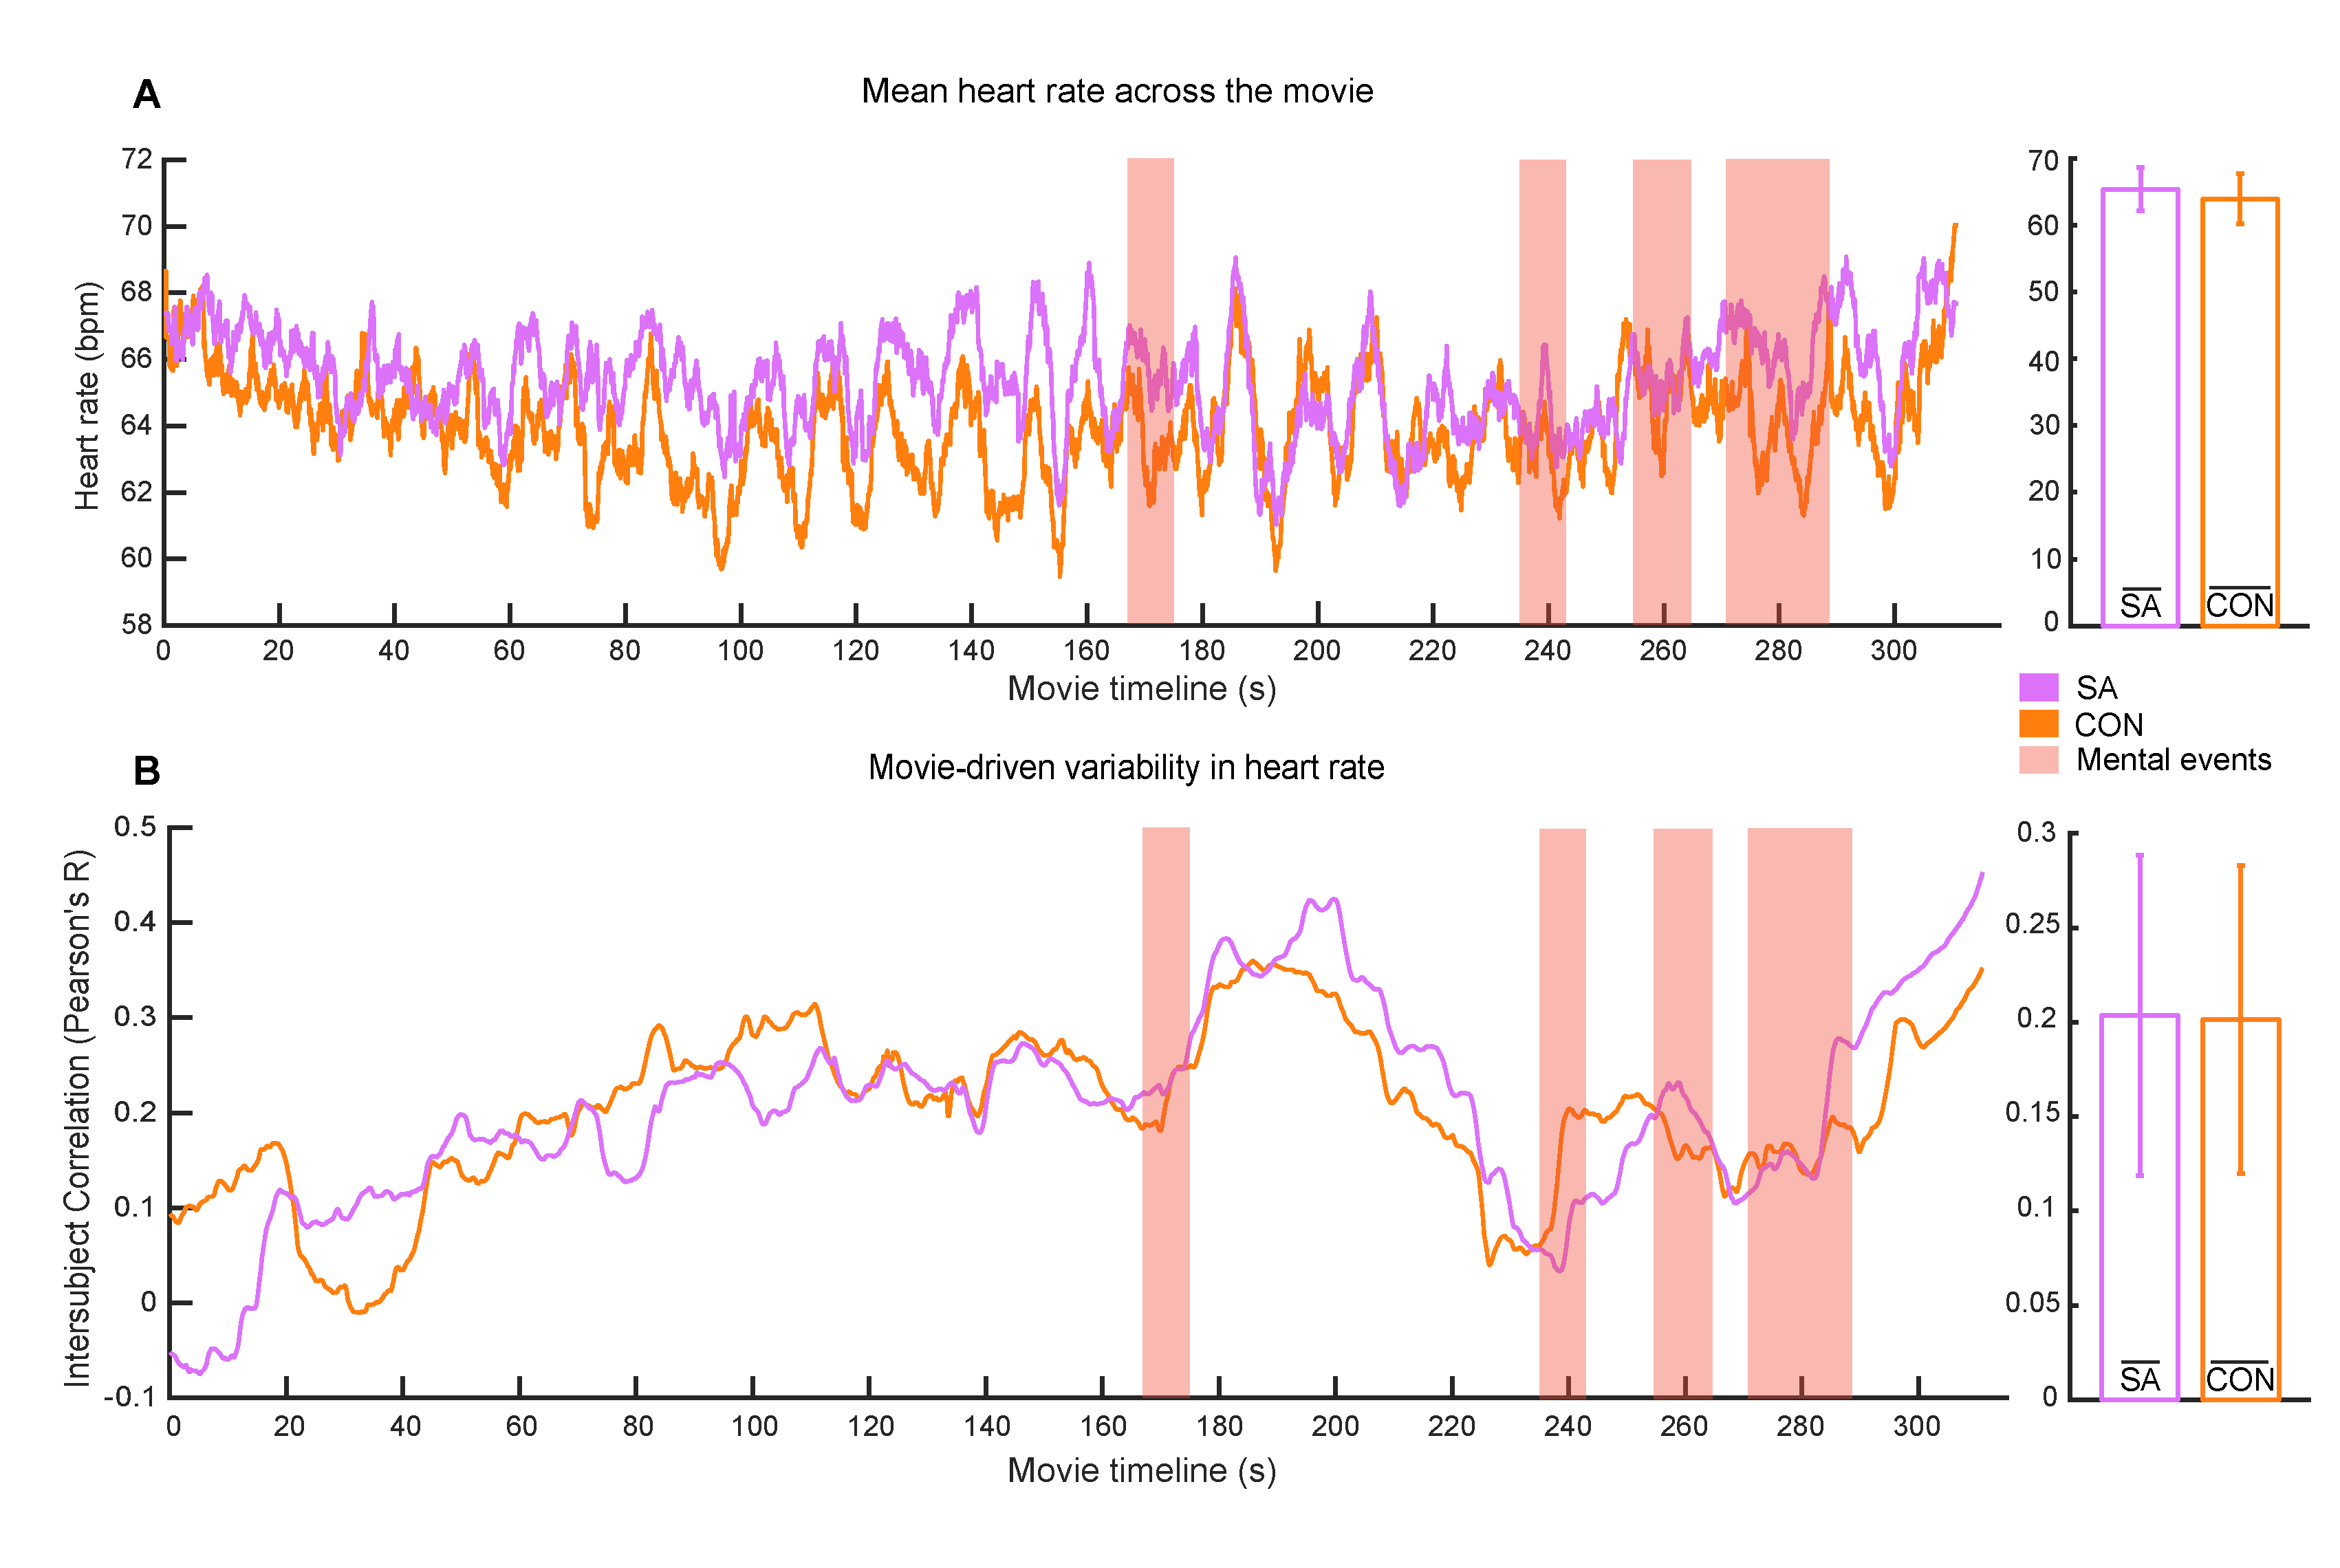
\includegraphics[width=1\textwidth]{./Chapters/03_MentalizingSA/Images/HeartRate.eps}}
	\caption{(a) Mean heart rate measured across the duration of the movie for both socially anxious and control participants. Adjacent histograms show the aggregated mean heart rate throughout the entire film for each group, with error bars representing 95\% confidence intervals. (b) Average intersubject correlation coefficients illustrate the intersubject variability in heart rate response during the movie among socially anxious and control participants. There were no significant differences detected in either metric between the two groups.}
    \vspace*{-10pt}
	\label{fig:heart-rate}
\end{figure}



\vspace{10pt}

\begin{figure}[!t]
	\centering
    \makebox[\textwidth][c]{\includegraphics[width=1\textwidth]{./Chapters/03_MentalizingSA/Images/ISCPupil.eps}}
	\caption{Dynamic intersubject correlation analysis revealed substantial fluctuations in variability throughout the film. Socially anxious participants exhibited lower correlations, indicative of higher variability in pupil responses compared to controls. Nonetheless, these differences did not reach statistical significance at any point during the viewing.}
    \vspace*{-10pt}
	\label{fig:isc-pupil-sa}
\end{figure}



% \afterpage{\blankpage}
% 
\chapter{Investigation of layer specific BOLD during visual attention in the human visual cortex}
\chaptermark{Layers in Spatial Attention}
\label{ch:attention}

\textcolor{gray}{{Tim van Mourik$^{1,*}$}, Peter J Koopmans$^{2,*}$, Lauren J Bains$^{1}$, David G Norris$^{1,2,\dagger}$, Janneke FM Jehee$^{1,\dagger}$\\
$^{1}$Radboud University Nijmegen, Donders Institute for Brain, Cognition and Behaviour, Nijmegen, The Netherlands \\
$^{3}$Erwin L. Hahn Institute for Magnetic Resonance Imaging, University Duisburg-Essen, Essen, Germany}\\

$^*$ 		{These authors contributed equally to this work}
$^\dagger$  {These authors contributed equally to this work}

%----------------------------------------------------------------------------------------
%	ABSTRACT
%----------------------------------------------------------------------------------------
\linespread{1.5}
\newpage
\section*{Abstract}
It is well-known that directing spatial attention towards a particular stimulus enhances cortical responses at corresponding regions in cortex. How attention modulates the laminar response profile within the attended region, however, remains unclear. In this paper, we use high field (7T) fMRI to investigate the effects of attention on laminar activity profiles in areas V1-V3; both when a stimulus was presented to the observer, and in the absence of visual stimulation. Replicating previous findings, we find robust increases in the overall BOLD response for attended regions in cortex, both with and without visual stimulation. Interestingly, when analyzing the BOLD response across the individual layers in visual cortex, we observed no evidence for laminar-specific differentiation with attention. We offer several potential explanations for these results, including theoretical, methodological and technical reasons.
\newpage
%----------------------------------------------------------------------------------------
\section{Introduction}
Directing visual attention to a location in the visual field typically improves behavioral sensitivity to stimuli presented at that location \cite{Posner1980,Lee1997,Yeshurun1998,Carrasco2004,Baldassi2005,Ling2009}. It is well known that these attentional benefits in behavior are accompanied by increases in BOLD response in early visual areas (e.g. \cite{Brefczynski1999,Gandhi1999,Kastner1999}), but how top-down processes modulate cortical responses at the laminar level remains unknown.

It is known from anatomical studies that the human cerebral cortex can be subdivided into histological layers with different cell types. The cytoarchitectonic structure varies across the brain and forms the basis of the Brodmann atlas, but almost all brain areas have six different histological layers \cite{Brodmann1909}. Although the precise function of each cortical layer remains unclear, their connectivity profile suggests a division in terms of bottom-up and top-down processing \cite{Felleman1991}. Specifically, Layer IV and to a lesser extent Layer V/VI are commonly associated with receiving feedforward drive from Layer III of lower cortical areas or from the thalamus \cite{Jones1998,Constantinople2013}. Layers I-II and VI, in contrast, are typically implicated in receiving downward information flow (feedback), which often originates from layer V \cite{Alitto2003}. Interestingly, this bottom-up versus top-down connectivity profile of each of the layers is to some degree paralleled in functional data. That is, from neurophysiological and neuroimaging work, it is known that various visual stimuli and tasks can exert differential effects on the various layers \cite{Maier2010,Xing2012,Self2013,VelezFort2014, OHerron2016}. Intracranial work in monkeys, for instance, shows that for selective attention and working memory (two functions that are commonly associated with top-down processes), current source density is increased in deep and superficial compared to middle layers in primary visual cortex \cite{VanKerkoerle2017}. Similar layer specific patterns have been shown in animal functional MRI. For instance, whisker stimulation led to an increase in BOLD response in Layer IV of rat barrel cortex, before such an enhancement was observed in any of the other layers, suggesting that layer IV was the first to receive feed forward drive from lower-level areas \cite{Yu2014}. In contrast, subsequent corticocortical connections in the same task appeared to activate Layers II-III and V in the motor cortex and contralateral barrel cortex before this affected any of the other layers, suggesting that these layers were the first to receive feedback signals. To what extent these results generalize to human cortex, however, remains to be investigated.

Recent advancements in fMRI have made it possible to also investigate the functional role of cortical layers in humans (e.g. \cite{Polimeni2010,Maass2014,Kok2016}). The human in vivo resolution with fMRI has increased to submillimetre voxel size. The thickness of the cerebral cortex varies between 1 and 4.5 millimetres \cite{Zilles1990,Fischl2000}, suggesting sufficient resolution to characterise activity across the individual layers. Indeed, some evidence suggests that human cortical activation can be measured with fMRI on a layer specific basis \cite{ Kok2016, Muckli2015}. For example, illusory contours, which are commonly associated with top-down processes, appear to activate the deep layers more than any of the other layers In area V1 \cite{Kok2016}, and some findings suggest that also specific activation of the middle layers can be measured with fMRI in human primary visual cortex \cite{Koopmans2010}.

While some neurophysiological evidence suggests a differential involvement of the cortical layers in top-down attention \cite{Nandy2017}, the effects of attention on the different layers in human visual cortex has remained unclear. Here, we examine with fMRI the potential influence of spatial attention on BOLD activity in the deep, middle and superficial layers in human visual areas V1, V2, and V3. Participants directed their attention to a cued location, and performed an attention-demanding task using an orientation stimulus that was shown at this location, while an unattended grating appeared at a different location of equal eccentricity. On some of the trials, subjects directed their attention to the cued location in anticipation of the stimulus, but no stimulus appeared at this location. Interestingly, although we observed a reliable increase of the overall BOLD response with attention across all layers, both with and without a stimulus present, we observed no differences in activation level between the layers due to attention. We provide several reasons for these surprising findings in the Discussion.

\section{Methods}
\subsection{Participants}
Nineteen healthy adults (aged 22-27, eight female), with normal or corrected-to-normal vision, participated in this study. All participants provided written informed consent in accordance with the guidelines of the local ethics committee. Two subjects were excluded from analysis; one subject was excluded due to insufficient (chance-level) performance on the attention task, and another due to weak retinotopic maps. The remaining data from 17 subjects were analyzed.

\subsection{Experimental design and stimuli}
Observers viewed the visual display through a mirror mounted on the head coil. Visual stimuli were generated by a Macbook Pro computer running MATLAB and Psychophysics Toolbox software \cite{Brainard1997,Pelli1997} and displayed on a rear-projection screen using a luminance-calibrated EIKI projector (resolution 1,024 X 768 pixels, refresh rate 60 Hz).

Participants were required to maintain fixation on a central bull's eye target (radius: 0.25\textdegree) throughout each experimental run. Each run consisted of an initial fixation period (3000 ms) followed by 32 stimulus trials (average duration: 4.7 seconds). Trials were separated by inter-trial intervals of variable duration (1000-2500 ms, uniformly distributed across trials). Each trial started with the presentation of a central attention cue (800 ms). This was followed by a delay period of variable duration (0-5000 ms; drawn from an exponential distribution to ensure a constant hazard rate), after which the two orientation stimuli appeared on the screen (500 ms). The orientation stimuli were followed by a response window (1300 ms), in which the fixation target turned orange.

Stimuli were two counterphasing sinusoidal gratings of independent orientation (\textasciitilde 45\textdegree~or \textasciitilde 135\textdegree; size: 7\textdegree; spatial frequency: 1 cycle per \textdegree; randomized spatial phase; contrast: 50\%; contrast decreased linearly to 0 towards the edge of the stimulus over the last degree), centered at 5\textdegree~to the left and right of fixation. We used a compound white/black cue consisting of two dots (dot size 0.25\textdegree) that straddled the fixation point (0.8\textdegree~to the left and right of fixation) to indicate with 100\% validity which of the two gratings should be attended \cite{Jehee2011}). Subjects were instructed to attend to the same side of fixation as either the white or black dot in the compound cue.

Participants were instructed to detect a small clockwise or counterclockwise rotation in the orientation of the grating at the attended location with respect to a base orientation at 45\textdegree~or 135\textdegree. The size of rotation offset was adjusted with an adaptive staircase procedure using QUEST \cite{Watson1983}, such that participants detected approximately 80\% of the offsets correctly. An overview of the experiment is shown in Fig.~\ref{fig:experiment}.

All but one participants completed 18 stimulus runs. The remaining participant completed 12 runs due to equipment failure.

Retinotopic maps of visual cortex were acquired in a separate scan session at a 3T scanner using conventional retinotopic mapping procedures \cite{Sereno1995,DeYoe1996,Engel1997}. 
\begin{figure}[!ht]
\centering
\includegraphics[width=1.0\textwidth, clip=true]{./Chapters/04_Attention/Images/Experiment}
\caption{Stimuli and experimental procedure. Example of a trial sequence from the experiment. Subjects fixated a central bull's eye target while gratings of independent orientation ($\pm$ 45\textdegree) appeared in each hemifield. A compound black/white cue indicated whether subjects should attend to the left or right stimuli; in this example, the white circle indicates `attend right.' Subjects had to discriminate near-threshold changes in orientation of the attended grating with respect to the closest diagonal. In one-third of trials, no stimuli appeared at either location. Red circles depict the attended location and were not present in the actual display.}
\label{fig:experiment}
\end{figure}

\subsection{MR data acquisition}
Functional images were acquired on a Magnetom Siemens 7T scanner with a 32-channel head coil (Nova Medical, Wilmington, USA) combined with dielectric pads \cite{Teeuwisse2012}, using a $T_2^*$-weigthed 3D gradient-echo EPI sequence \cite{Poser2010} (TR/TE/$\alpha$=3060 ms/20 ms/14\textdegree, 72 slices oriented orthogonally to the calcarine sulcus, voxel size [0.8 mm]$^3$, FOV: [192 mm]$^2 $, GRAPPA factor 8).

Gradient maximum amplitude was 40 mT/m (in practice, however, this maximum wasn't reached), the minimum gradient rise time was 200 $\mu$s, and the maximum slew rate was 200 T/m/s. Shimming was performed using the standard Siemens shimming procedure for 7T. There were 18 runs of 72 $\pm$ 4 volumes. As the lengths of the events and the inter trial interval were of unequal length, there was a small variation in the number of volumes per run.

Finger pulse was recorded using a pulse oximeter affixed to the index finger of the left hand. Respiration was measured using a respiration belt placed around the participant's abdomen.

Anatomical images were acquired using an MP2RAGE sequence \cite{Marques2010} [0.75 mm]$^3$, yielding two inversion contrasts (TR/TE/TI1/TI2 = 5000 ms/1.89 ms/900 ms/3200 m).

In a separate session prior to the main experiment, a retinotopy session was conducted at a Siemens 3T Magnetom Trio scanner. A high-resolution T$_1$-weighted anatomical scan was acquired (MPRAGE, FOV 256 $\times$ 256, 1 mm isotropic voxels) at the start of the session. Functional images were subsequently collected using T$_2^*$-weighted gradient echo EPI, in 30 slices oriented perpendicular to the calcarine sulcus (TR/TE/$\alpha$ = 2000 ms/30 ms/90\textdegree, FOV = 64 $\times$ 64, [2.2 mm]$^3$ isotropic resolution).


\subsection{Functional MRI preprocessing}
\subsubsection{Data preprocessing}
\label{sec:dataProcessing}
Data were corrected for subject motion using SPM with the mean functional volume across time as a reference \cite{Friston1995}. Residual motion-induced fluctuations in the BOLD signal were removed through linear regression, based on the alignment parameters of SPM. Scanner drifts were corrected via linear regression with high-pass filter regressors to filter out frequencies below 1/64 Hz. Pulsating signals as a result of the respiratory and cardiac cycle were removed as follows. The cardiac/respiratory peaks were automatically detected from the physiological recordings using in-house interactive peak-detection software, and manually corrected where needed. With a custom MATLAB implementation of RETROICOR \cite{Glover2000}, fifth order Fourier regressors were constructed for heart rate and respiration and subsequently removed from the functional images via linear regression. A small part (10\% of respiratory measurements, and 18\% of heart rate measurements) was of insufficient quality and could not be used in this analysis. Functional data for these time frames were used in the main analysis but uncorrected for cardiac and respiratory noise.

The functional and anatomical scans were brought to the same space by registering the anatomical surface from the retinotopy session to the mean functional volume using boundary based registration (BBR), implemented in FreeSurfer's \texttt{bbregister} \cite{Greve2009}. All registration results were inspected and manually refined when necessary. Where needed, registration was improved by an additional pass of BBR using an in-house MATLAB implementation. Local distortions in EPI due to field inhomogeneity were corrected by means of recursive boundary registration \cite{VanMourikISMRM2014}, which recursively applies BBR to small portions of the cortical surface to correct topology locally by means of optimizing the grey-white matter contrast along the surface.

Because of temporal changes in magnetic field inhomogeneities, local topology slightly changed over the course of the entire session. For this reason, the 18 functional runs obtained for each subject were first divided in three groups of each 6 contiguous runs, and then each group was pre-processed separately.  Time courses were subsequently concatenated before entering the main analyses.


\subsubsection{Regions of Interest}
Regions of interest (areas V1, V2, V3) were defined on the reconstructed cortical surface using standard retinotopic mapping procedures \cite{Sereno1995,DeYoe1996,Engel1997}. After identifying areas V1-V3, data were smoothed along the reconstructed cortical surface with a Gaussian kernel (FWHM: 4 mm). The smoothed version of the data was only used in region of interest selection, and not in the main analysis. In each area, we then selected the 600 vertices that responded most strongly to the stimulus (shown on the cortical surface in Supplementary Figure~\ref{SM5}). The selected vertices were resampled from the cortical surface back to subject space by means of FreeSurfer's \texttt{label2vol}. T-values of selected voxels ($\mu \pm \sigma$) were V1: $T=2,989 \pm 0.854$, V2: $T=2.317 \pm 0.689$ and V3: $T=2.117 \pm 0.713$). Note that the selection of voxels based on visual activation per se is orthogonal to the analysis of interest, which addresses the effects of attention on individual layers in cortex. Control analyses verified that our results were not strongly affected by the number of vertices selected for subsequent analysis (See Supplementary Figures).

\subsection{Cortical profile extraction}
Layer specific signals were obtained by means of a layer specific spatial General Linear Model (GLM) as proposed by \cite{VanMourikISMRM2015} and briefly described in \cite{Kok2016}. Specifically, we applied the level set method \cite{Sethian1999} on the reconstructed cortical surface \cite{Dale1999} to create a cortical layering of three equivolume layers, following the procedures described in \cite{Waehnert2014}. The gradient and the curvature of the cortex were defined as a function of Laplacian streamlines in the grey matter as this more naturally follows the structure of cortical columns \cite{Leprince2015}. Partial volume inaccuracies were adjusted for by explicitly taking into account the orientation of the voxel with respect to the cortex \cite{VanMourikISMRM2015}. This procedure enabled us to divide the gray matter in three equivolume cortical layers, which amounts to roughly one voxel per layer. We additionally defined a volume on either side of these three cortical layers to capture signals for white matter and cerebrospinal fluid. On the basis of  these definitions, we then created a laminar (spatial) design matrix. By regressing this design matrix against the functional data within an ROI, we obtained laminar time courses. In the regression, we used generalised least squares to account for spatial covariance in the noise. The voxel-to-voxel covariance matrix was defined based on Gaussian noise spread (FWHM 1.41 mm) between neighbouring voxels. 

\subsection{Statistical Analyses}
Temporal linear regression was used to compare between the experimental conditions. Regressors were created as follows. The stimuli appeared during the stimulus window on 2/3rds of trials, which were modeled with a single regressor (stimulus \emph{on}). The remaining stimulus windows were also modeled with a regressor (stimulus \emph{off}). In addition, attention could either be directed to the \emph{left} or \emph{right} visual field; these conditions were each modeled with a regressor. We so obtained four regressors for each of the conditions of interest. To remove any potential influence from the anticipation period, i.e. before stimulus presentation, we additionally included separate regressors for each of these four factors during the anticipation window. We used a canonical HRF (parameters: time-to-peak-parameter: 5 second) to model the fMRI responses. To verify the appropriateness of this function, a finite impulse response (FIR) analysis \cite{Josephs1997} was performed using the data from four pilot subjects (not included in the current study). Based on this pilot data set, temporal or dispersion derivatives were not included into the statistical model. The baseline signal of each run was captured by adding a regressor column of ones for each run separately. As described above (Sec.~\ref{sec:dataProcessing}), the data were pre-processed by means of nuisance regression. This was performed by adding the nuisance regressors to the design matrix, effectively adjusting for the statistical loss in degrees of freedom as a result of nuisance regression. The reference of one percent signal change was the height of a peak of a two-second-long isolated event \cite{Mumford2007}.

The temporal regression was performed on the previously extracted layer-specific time courses. The obtained parameter estimates were divided by their baseline estimates, in order to convert them to percent signal change. The values in percent signal were compared at the group level by means of ANOVAs and t-tests as appropriate. As the experiment was left-right symmetric and we found no differences between hemispheres in the analyses of interest, the hemispheres were treated as two measurements per participant.

\subsection{Code availability}
All functions for laminar analysis that are mentioned here are available on \url{https://github.com/TimVanMourik/OpenFmriAnalysis}. Custom analysis scripts are available on request. The analysis scripts were made with Porcupine pipeline software available on \url{http://timvanmourik.github.io/Porcupine} \cite{VanMourik2017}.



\section{Results}
Subjects generally performed well at the orientation discrimination task. The mean orientation discrimination threshold across participants was 6.6\textdegree, and behavioral performance was quite stable across runs.

\subsection{Spatial attention increases fMRI response amplitudes}
First, we determined whether directing attention to a spatial location led to stronger overall responses in the visual cortex. Regions of interest consisted of voxels that were significantly activated by the stimulus in all layers of areas V1, V2, and V3 (see Methods). We compared the amplitude of the BOLD response with and without attention, for trials in which a stimulus was presented and those in which no stimulus appeared (see Fig.~\ref{fig:roiresults}). Data were analyzed using a general linear model with area, attention (attended vs. unattended), and stimulus (present vs. absent) as factors (see Methods). We first focused on the effects of attention per se. Attention significantly enhanced the BOLD response at the attended location in areas V1-V3 (effect of attention, F(1, 16) = 43.4, p = 6.36$\cdot10^{-6}$), with a trending increase in attention-based activity for higher-level areas (interaction between attention and area, F(2, 32) = 2.63, p = 0.088). The mean effect sizes (in percent signal change) were 0.41\%, 0.64\% and 0.59\% for V1, V2, and V3 respectively, and slightly stronger to those reported before \cite{Murray2008,Jehee2011}. Next, we investigated whether the effects of attention depended on the presence of a visual stimulus. Specifically, we compared attentional effects between trials in which observers were expecting a stimulus but none was presented, and trials in which the stimulus did appear on the screen. Replicating previous reports \cite{Kastner1999}, the effect of attention in areas V1-V3 was not significantly different in the absence compared to presence of visual stimulation (two-way interaction between and attention and stimulus, F(1, 16) = 0.26, p = 0.585), with no reliable change across areas (three-way interaction between stimulus, attention and area, F(2, 32) = 0.026, p = 0.901). Thus, attending to a spatial location enhances the BOLD response at that location, even in the absence of visual stimulation.
\begin{figure}[!ht]
\centering
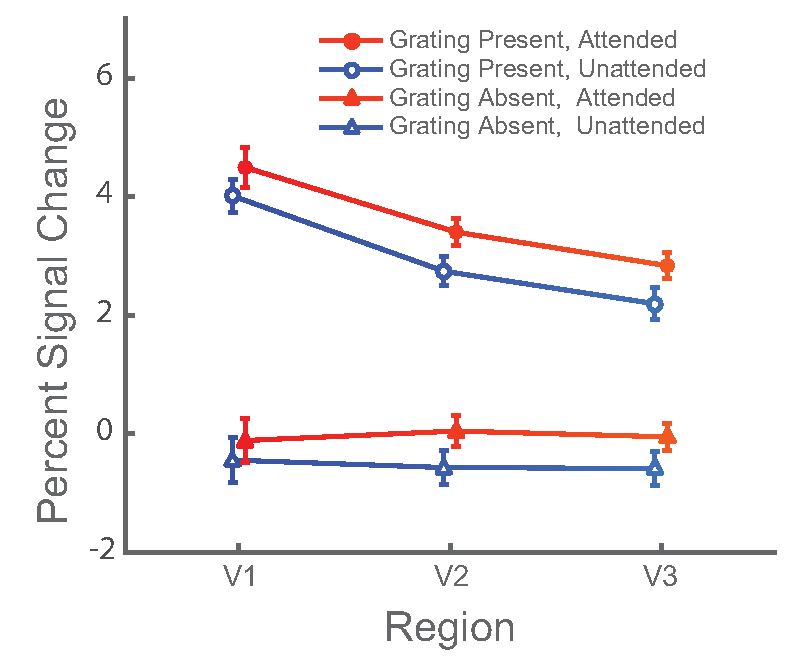
\includegraphics[width=0.8\textwidth, clip=true]{./Chapters/04_Attention/Images/RoiResults}
\caption{Amplitude of the BOLD response for attended and unattended regions in areas V1-V3. Red lines indicate the attended condition, blue the unattended. The top lines (circles) show the response when a grating was presented, the bottom lines (triangles) when no grating was presented, at the attended or unattended location. Response amplitudes were significantly higher for attended than unattended locations and stimuli. Error bars indicate $\pm$1 SEM.}
\label{fig:roiresults}
\end{figure}

\subsection{Spatial attention increases responses across the layers}
Next, we asked whether attention led to changes in the pattern of activity across cortical layers in these areas. We used a spatial general linear model (see methods) to first characterize activity in each of three distinct cortical layers. Data were subsequently analyzed using a temporal general linear model with attention, stimulus, area, and layer as factors (see Methods). Consistent with previous studies \cite{Koopmans2010,Polimeni2010}, we found a general increase in BOLD response from white matter to pial surface (see Fig~\ref{fig:layerresults}, overall effect of layer, F(2, 32) = 12.5, p = 9.85$\cdot10^{-5}$). This increase in BOLD response with decreasing distance to the pial surface was reliably larger in the presence of a stimulus (two-way interaction between layer and stimulus, F(2, 32) = 61.1, p = 1.00$\cdot10^{-11}$), and was significantly different between the three areas (three-way interaction between layer, stimulus, area: F(4, 64) = 3.33, p = 0.015; post hoc analyses revealed a trending larger effect for area V1 compared to V2 (T(16) = 2.11, p = 0.051), and a larger effect for area V2 compared to areas V3 (T(16) = 3.37, p = 0.0039). This tendency of the BOLD response to increase from lower layers to higher layers should be interpreted with caution, however, as blood flows from the gray-white matter boundary towards the pial surface. Hence, any change in BOLD response that arises in layers V-VI will automatically affect the BOLD response in downstream layers. This accumulation of signal may also result in a larger slope of activation through the layers for larger effects with equal laminar activation, thus explaining the greater layer by stimulus interaction in earlier visual regions. In contrast to the layer-specific increase in BOLD signal when presenting a stimulus, we found no significant change in the effects of spatial attention across the layers (two-way interaction between layer and attention, F(2, 32) = 2.33, p = 0.114). This may reflect equal activation of all layers, or a rather shallow slope as a result of low attentional effect. Next, we determined whether the layer-specific increase in BOLD signal with attention was distinct from the observed stimulus-based effects. The attention-based increase in activity was indeed reliably different from stimulus-driven changes in layer response (post hoc comparison between layer by stimulus effect and layer by attention effect; T(16) = 4.94, p = 1.47$\cdot10^{-4}$). However, this effect should be interpreted with caution, as the strength of the layer responses is tightly coupled to the strength of the main effects. In addition, there was no reliable difference between the effects of attention versus stimulus between any of the three layers (three-way interaction between layer, stimulus and attention, F(2, 32) = 1.69, p = 0.200). Control analyses established that these results were not strongly affected by the number of voxels included in the analyses (Supplementary Figures~\ref{fig:layerresults300}-\ref{fig:layerresults900}), nor by the number of layers analyzed (Supplementary Figure~\ref{fig:layerresults4layers}). In addition, these results did not qualitatively change when layer activation profiles were defined using volume interpolation (Supplementary Figure~\ref{fig:layerresultsinterp}). Moreover, combining the anticipation (i.e., time frame prior to when a stimulus could appear, see Figure~\ref{fig:experiment}) and stimulus windows in the analyses did not reliably affect any of these results (Supplementary Figure~\ref{fig:layerresultsplusattention}). Thus, while the overall effects on BOLD activity of both visual stimuli and attention were rather robust and similar to previously reported values for visual cortex \cite{Kastner1999,Jehee2011, Koopmans2010}, no differential pattern of activity was observed between these two processes across the visual cortical layers.
\begin{figure}[!ht]
\centering
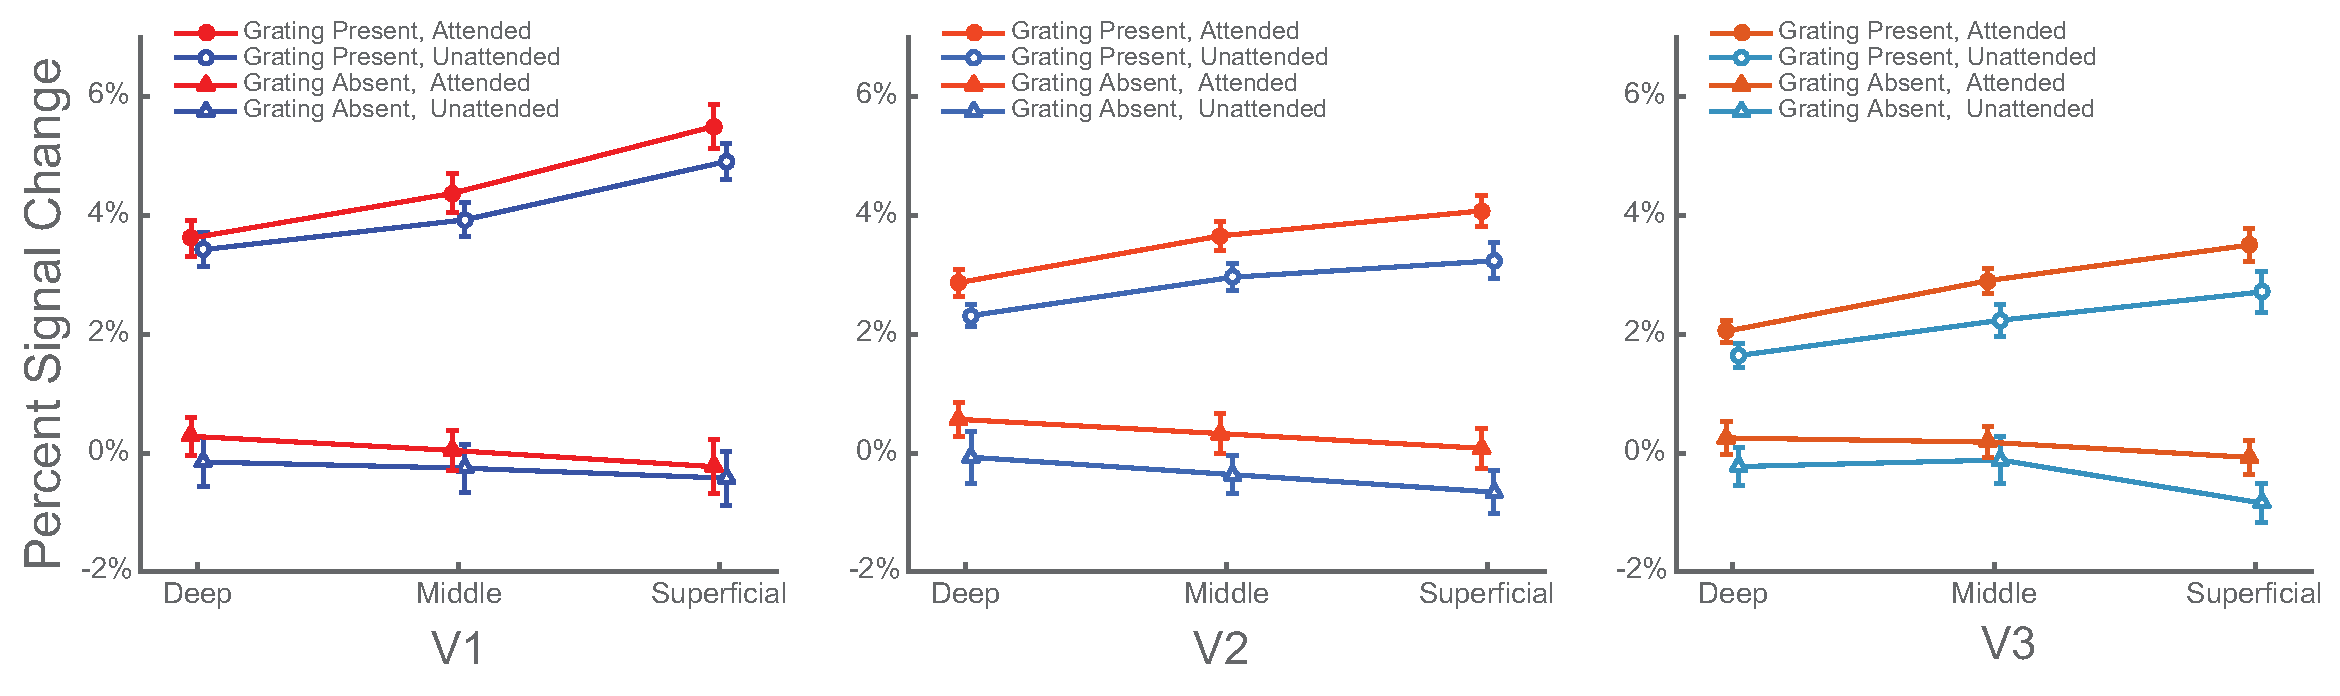
\includegraphics[width=0.8\textwidth, clip=true]{./Chapters/04_Attention/Images/LayerResults}
\caption{Layer-specific amplitude of the BOLD response in the experiment in areas V1-V3. Circles indicate when a grating was presented, squares depict when no grating was presented, at either the attended (red) or unattended (blue) location. When a stimulus was presented, activation reliably increased towards the pial surface. Attention significantly enhanced the BOLD response across all layers. Error bars indicate $\pm$1 SEM.}
\label{fig:layerresults}
\end{figure}




\section{Discussion}
This study investigated the effects of spatial attention on the BOLD signal measured from individual layers in early visual cortex. Focusing first on the overall amplitude of the BOLD response in all layers combined, we found that attending to a stimulus reliably and substantially increased the BOLD signal in early visual areas, both when a stimulus was presented to the observer and in the absence of physical stimulation (cf. \cite{Kastner1999,Murray2008,Li2008}). Moreover, and much in line with earlier results on layer-specific activation patterns in visual cortex (\cite{Polimeni2010,Koopmans2010}), we observed a general increase in activation towards the superficial layers - one that is commonly explained by gradient echo being more susceptible to the draining veins on the pial surface. Interestingly, and much to our surprise, we observed no differential activity in the individual layers when comparing between top-down (attention-driven) and bottom-up (stimulus-driven) activity - a finding that stands in notable contrast to previous observations \cite{Kok2016}. We identify several potential reasons for this absence of layer specific differentiation that we outline and discuss below.
	
One possibility is that our data are simply insufficiently robust for showing a significant difference in activity across depth between the two conditions. It is well known that the BOLD signal includes multiple sources of noise related to both MRI scanner and participant, and this holds especially true for signals recorded at the sub-millimeter scale. For example, at a resolution this high, even the smallest movement of the participant may cause additional blurring of the data, with potentially detrimental effects on the signal-to-noise ratio. For this reason, we collected data from 17 participants - a sample size much larger than typical in attention-based fMRI studies at standard spatial resolution (cf. N=4-6 in\cite{Kastner1999,Kamitani2005,Jehee2011}), and it is even in the larger range for layer-based fMRI studies at high resolution (cf. N=6 in \cite{Polimeni2010}, N=4 in \cite{Muckli2015}, N=10 in \cite{Kok2016}). To minimize the effects of various sources of noise, we took great care in measuring and removing physiological artifacts, and further improved existing layer extraction techniques by developing a novel spatial general linear model that separates laminar signal from different layers instead of sampling a mixed interpolation of the layers. Additionally, we ensured that similar results were obtained using more conventional layer-extraction procedures. Indeed, the combined success of these procedures is well illustrated by the effect sizes observed in the current study for both stimulus presentation (4.5\%, 3.3\%, 2.8\% in V1, V2 and V3) and attention (0.41\%, 0.64\%, 0.59\% in V1, V2 and V3), which are comparable or higher to those reported in previous publications \cite{Murray2008,Jehee2011}. There are, however, some differences in experimental design between our study and previous laminar investigations that could potentially account for the incongruity in results. Because we were interested in the degree to which top-down processes could be dissociated from feed forward stimulation with fMRI, we directly contrasted between these two conditions in our analyses. Previous studies, on the other hand, have focused on top-down activity in isolation (e.g. \cite{Muckli2015, Kok2016}), or used multi-voxel pattern analyses - rather than overall BOLD amplitude, to compare between conditions \cite{Muckli2015}. \cite{Kok2016}, for example, directly compared between the overall activation levels in individual cortical layers, and found a significant difference in BOLD activity due to recurrent signals that were evoked by an illusory stimulus. It will be interesting for future studies to address the degree to which these experimental factors can account for the disagreement in results between our and previous work.

An alternative explanation for the incongruity in results could lie in attention itself, which may be mediated by mechanisms distinct from previously investigated processes. That is, previous work using high-resolution fMRI focused not on spatial attention, but rather on figure-ground segregation \cite{Kok2016} and other non-classical receptive field effects in cortex \cite{Muckli2015}. It is conceivable that these modulatory processes operate on the individual cortical layers in a manner dissimilar from the attentional mechanisms studied here. It is known from primate studies, for example, that attention increases the response gain of neurons in visual cortex \cite{Treue1999,MartinezTrujillo2004} - such an increase in attentional gain could lead to general enhancements in neural activity irrespective of cortical layer, as we have observed here.
	
Regardless of the potential reasons for the disparity between current and previous results, we believe our study presents an important message to a field that is currently in its nascent stages of development. We hope that the results and procedures detailed here will help move the field forward and resolve which experimental parameters are paramount, and which are not, to detecting differential activity between individual layers in human visual cortex with high-resolution fMRI.

\section{Author contributions}
PJK and JFMJ designed the experiment. TvM and LJB collected the data. TvM and DGN developed the laminar analysis techniques. TvM and JFMJ analysed the data. TvM, DGN, and JFMJ wrote the paper. 

\section{Acknowledgements} 
Tim van Mourik acknowledges support by the Spinoza grant [SPI 40-118].
\section{Supplementary Materials}
\setcounter{figure}{0}
\begin{figure}[!ht]
\centering
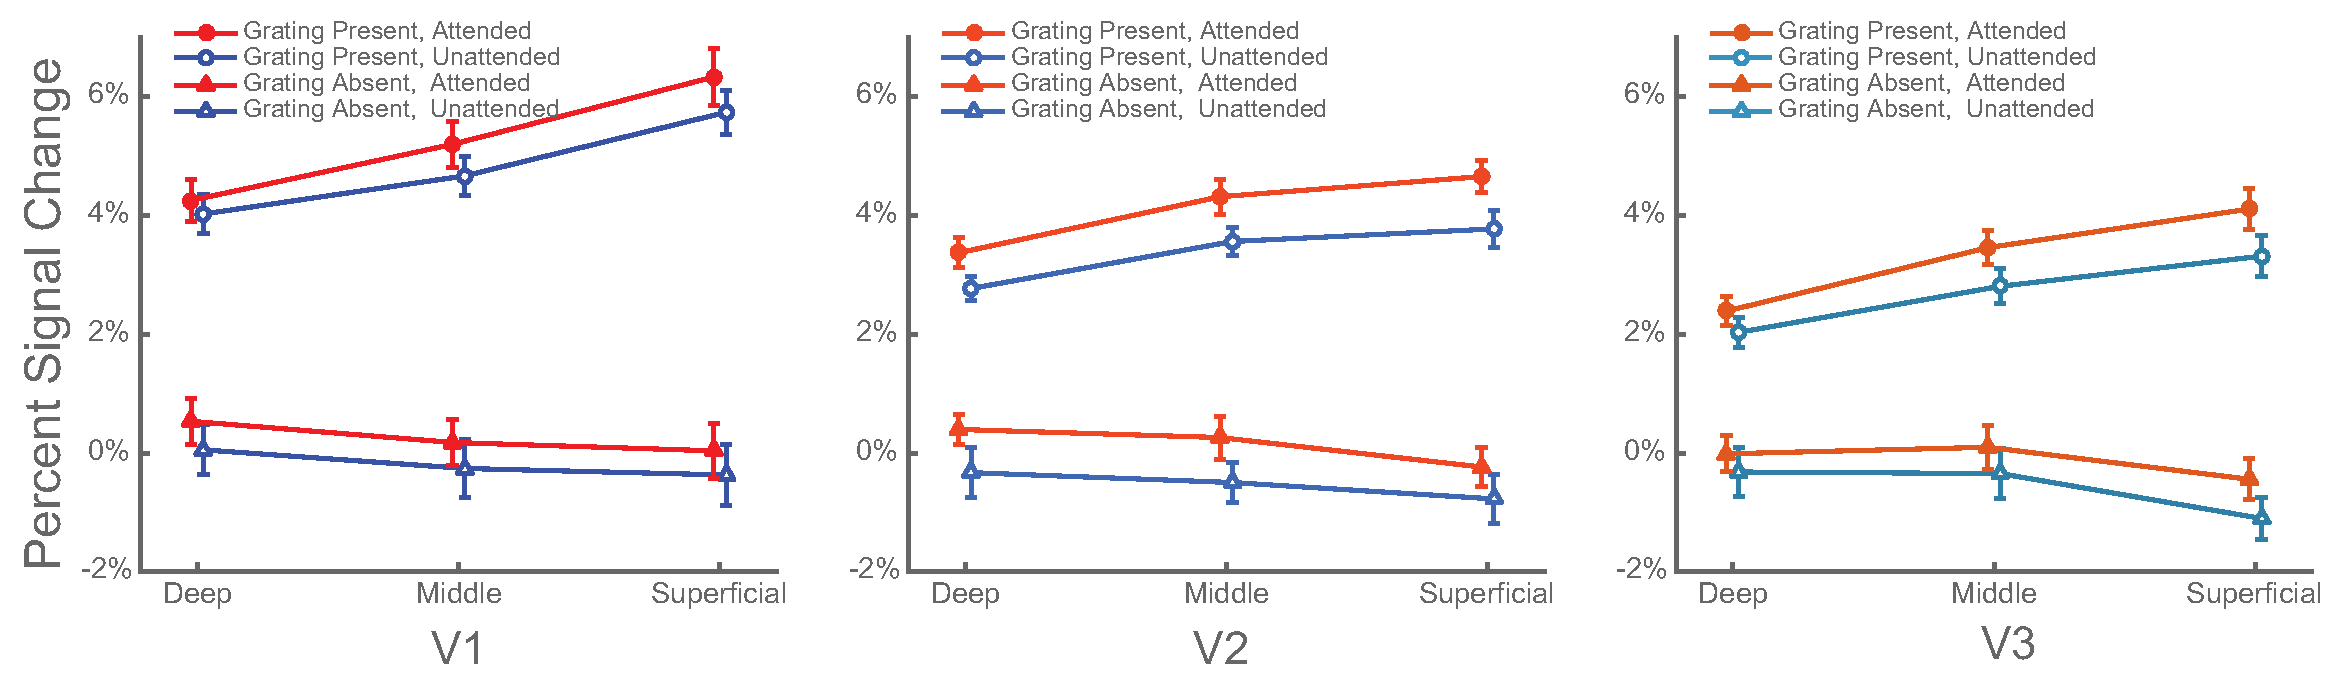
\includegraphics[width=1.0\textwidth, clip=true]{./Chapters/04_Attention/Images/SM_LayerResults_300vertices}
\caption{Control analysis of an ROI with the 300 highest activated vertices.}
\label{fig:layerresults300}
\end{figure}
\begin{figure}[!ht]
\centering
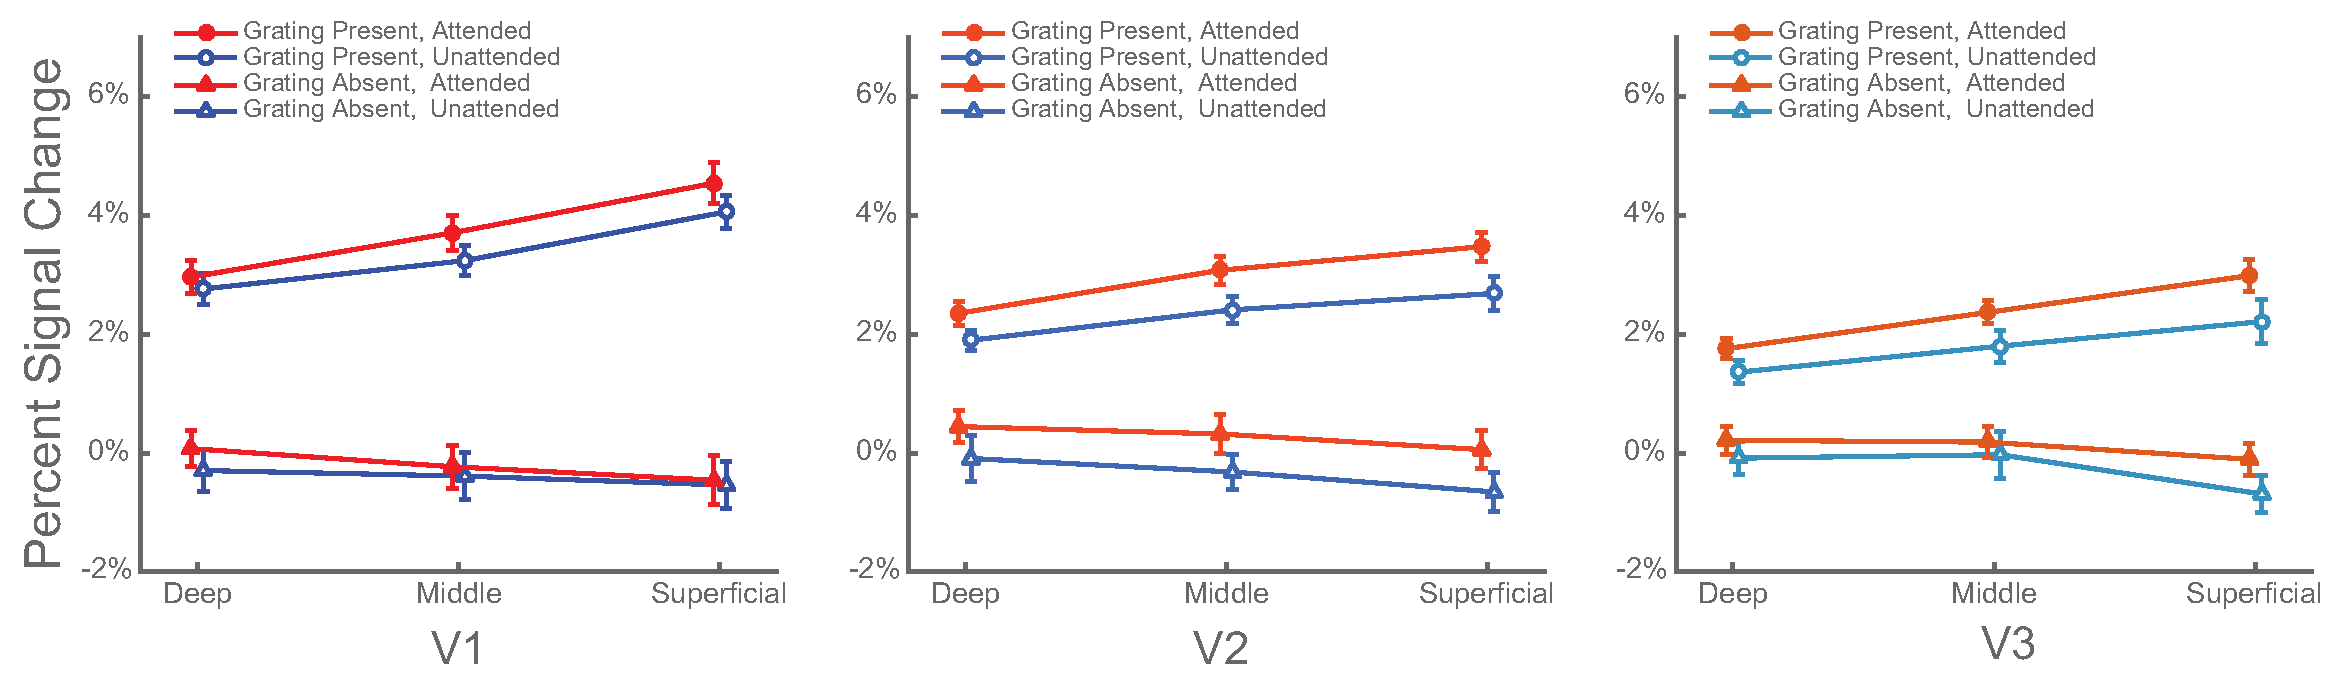
\includegraphics[width=1.0\textwidth, clip=true]{./Chapters/04_Attention/Images/SM_LayerResults_900vertices}
\caption{Control analysis of an ROI with the 900 highest activated vertices.}
\label{fig:layerresults900}
\end{figure}
\begin{figure}[!ht]
\centering
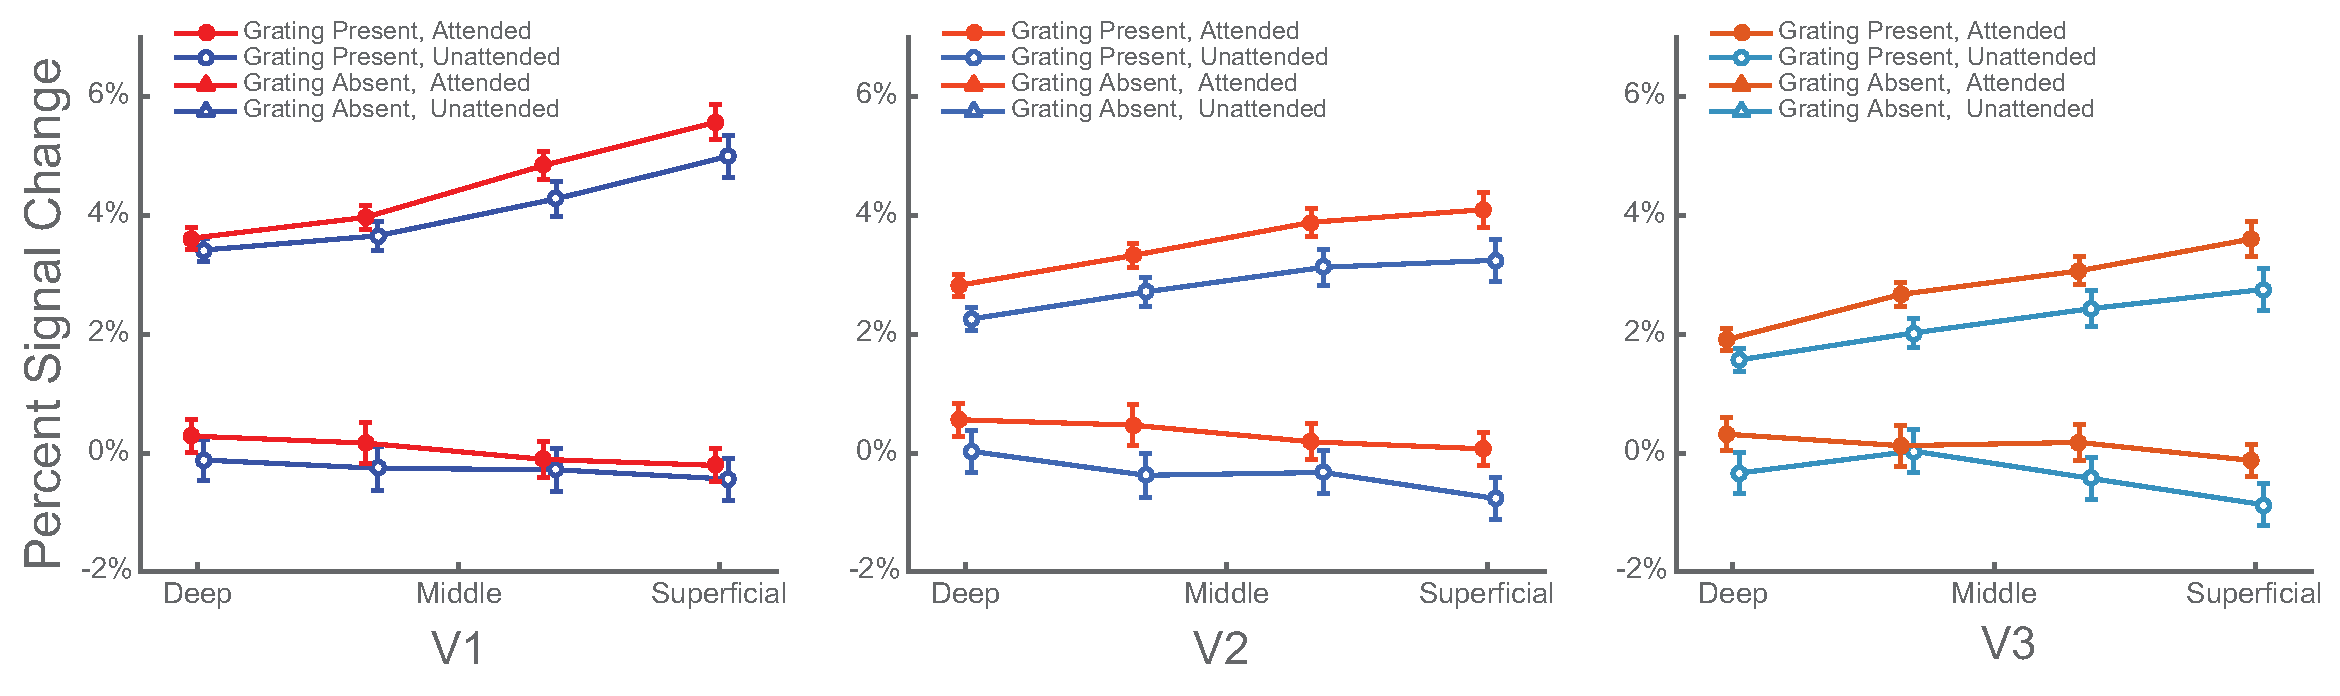
\includegraphics[width=1.0\textwidth, clip=true]{./Chapters/04_Attention/Images/SM_LayerResults_4Layers}
\caption{Control analysis of an ROI with the 600 highest activated vertices, within each of 4 layers.}
\label{fig:layerresults4layers}
\end{figure}
\begin{figure}[!ht]
\centering
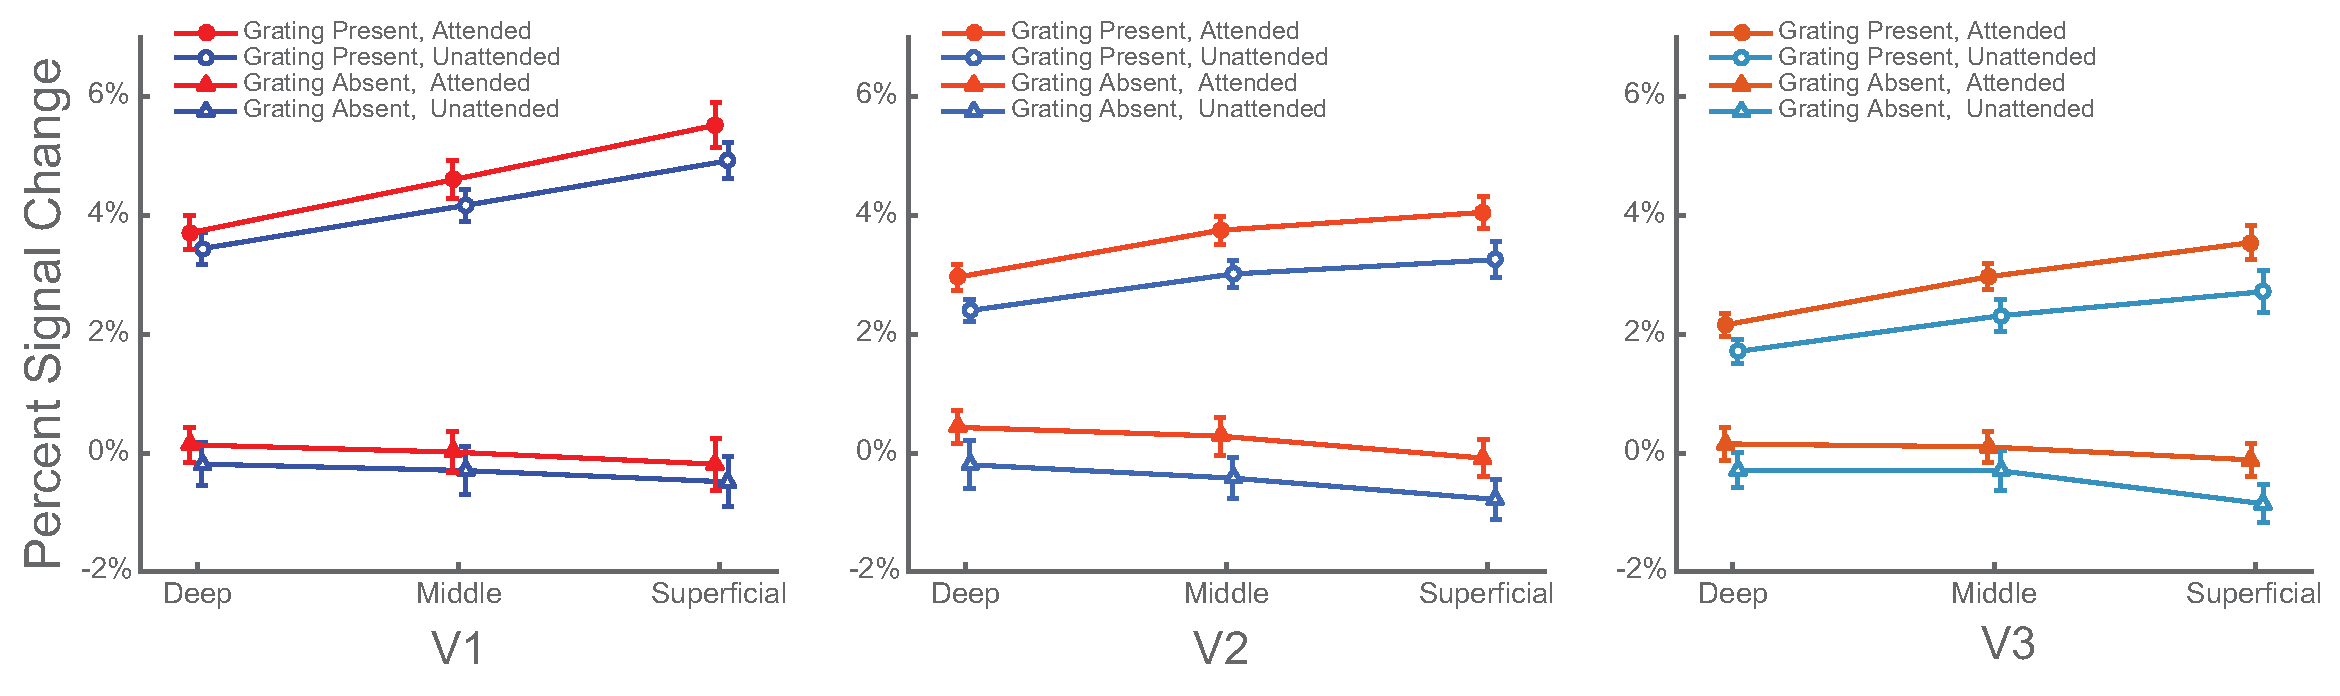
\includegraphics[width=1.0\textwidth, clip=true]{./Chapters/04_Attention/Images/SM_LayerResults_interpolation}
\caption{Control analysis of an ROI with the 600 vertices highest activated vertices, where the laminar signal was obtained by means of interpolation instead of a laminar spatial GLM.}
\label{fig:layerresultsinterp}
\end{figure}
\begin{figure}[!ht]
\centering
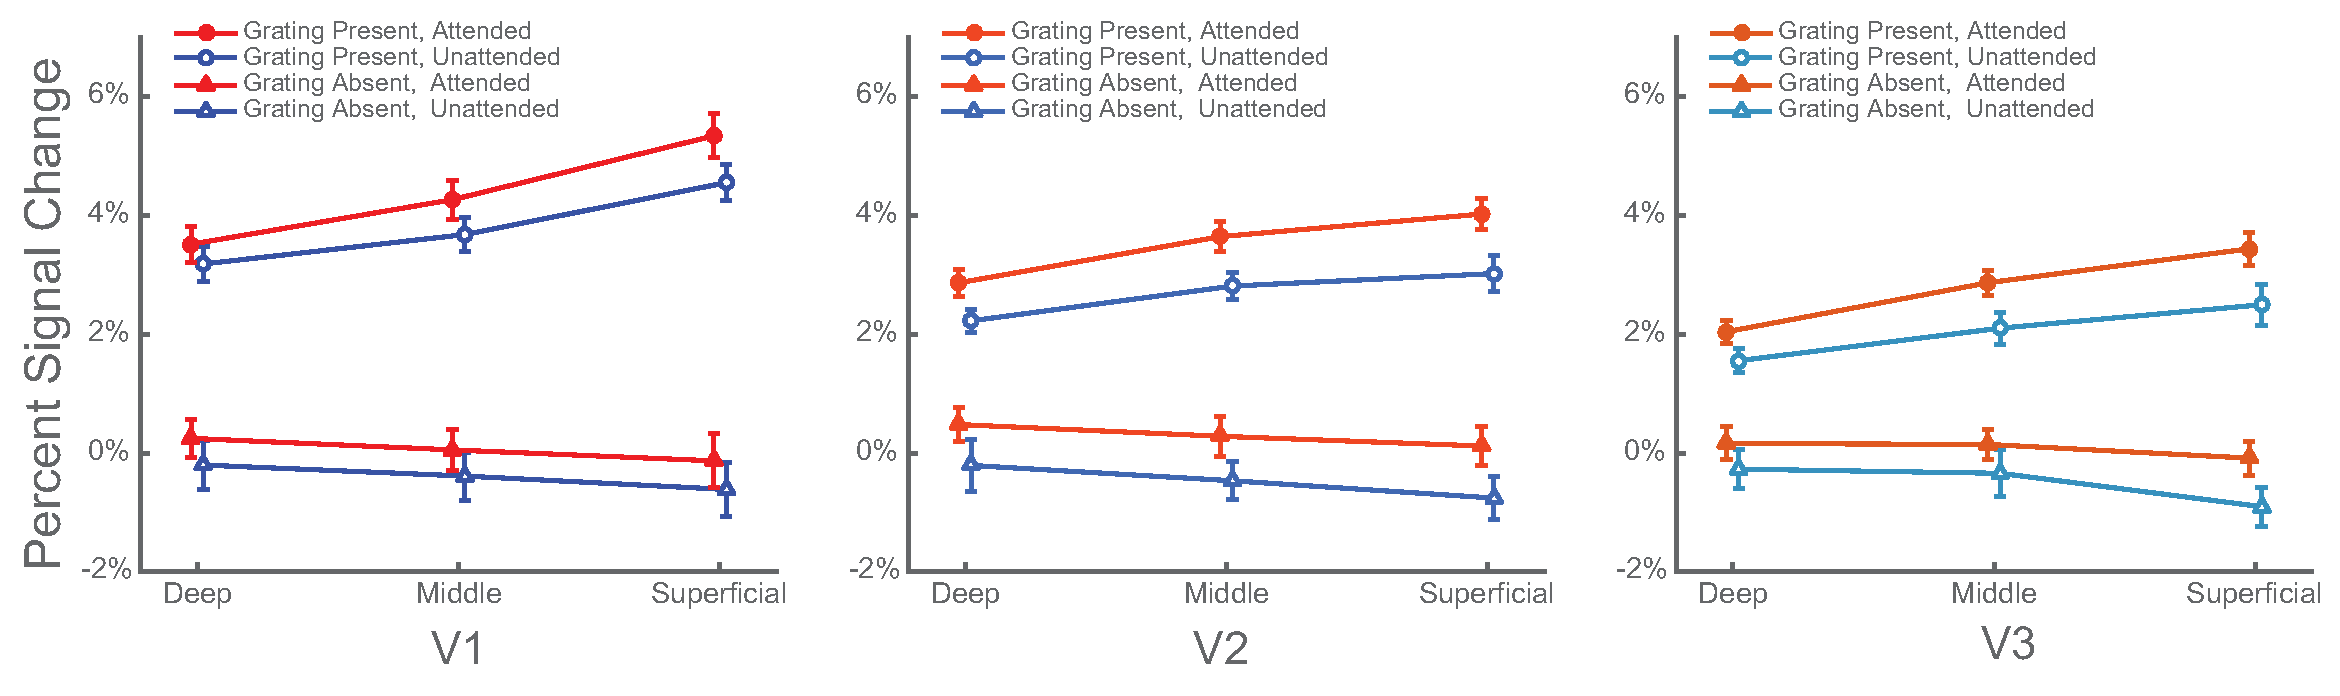
\includegraphics[width=1.0\textwidth, clip=true]{./Chapters/04_Attention/Images/SM_LayerResults_plusAttention}
\caption{Control analysis of an ROI with the 600 vertices highest activated vertices, where the signal from the anticipation window was added to the signal from the stimulus window.}
\label{fig:layerresultsplusattention}
\end{figure}
Figure S1-5. Layer-specific amplitude of the BOLD response in areas V1-V3. Figures S1 and S2 show stimulus and attention-based effects across layers after selecting, respectively, the 300 and 900 most activated vertices (cf. Fig.~\ref{fig:layerresults} in the main text). Figure S3 shows results after defining four cortical layers, rather than three, and Figure S4 depicts results obtained from interpolation instead of a laminar spatial GLM. Error bars indicate $\pm$1 SEM. For figure S5, the signal from the anticipation window was added to the signal from the stimulus window. In all Figures, presenting a stimulus (circles) resulted in a reliable increase in BOLD response from deep to superficial layers. The BOLD response was significantly enhanced for attended locations (red) compared to unattended location (blue) across layers, both when a stimulus was presented and in the absence of visual stimulation. There were only two instances where significance changed compared to the layer analyses that are presented in the main text. The Attention by Layer interaction was not significant in the main analysis (p = 0.114), but was significant in the control analysis when interpolation was used (p = 1.50$\cdot10^{-4}$) and when the signal from the anticipation window was added (p = 0.019). While the Stimulus by Layer by Area interaction was significant in the main analysis (p = 0.015), this interaction failed to reach significance after selecting the 900 most activated vertices (p = 0.12), or when repeating the analysis using four (rather than three) layers (p = 0.056). All other reported results are qualitatively similar to the findings in the main text.
\label{SM5}
\begin{figure}[!ht]
\centering
\includegraphics[width=0.6\textwidth, clip=true]{./Chapters/04_Attention/Images/ExampleBrain}
\caption{Example of Regions of interest on the inflated cortical surface for a representative subject. The label contours from top to bottom show dorsal V3, V2, and V1 and ventral V1, V2, and V3, in both hemispheres. The 600 most activated vertices (highlighted) per region where selected for the main analysis, the 300 and 900 vertices for control analyses in order to show that the effects are independent of size of region of interest.}
\label{fig:roifigures}
\end{figure}
%Random Subject19


%300 vertices:
%The T-values in the region of interest ($\mu \pm \sigma$) were for V1 $T=3.414 \pm 0.950$, for V2 $T=2.728 \pm 0.726$ and for V3 $T=2.562 \pm 0.779$.


%900 vertices:
%The T-values in the region of interest ($\mu \pm \sigma$) were for V1 $T=2.637 \pm 0.828$, for V2 $2.002 \pm 0.715$ and for V3 $1.773 \pm 0.716$.



%A visualisation of the workflow is shown in Fig.~\ref{fig:workflow}.
%\input{./Chapters/04_Attention/Chapters/Figures/FigureWorkflow}





% \afterpage{\blankpage}
% 
\chapter{Porcupine: a visual pipeline tool for neuroimaging analysis}
\chaptermark{Porcupine}
\label{ch:porcupine}

\textcolor{gray}{{Tim van Mourik$^{1}$}, Lukas Snoek$^{2}$, Tomas Knapen$^{3,4}$, David G Norris$^{1,2}$\\
$^{1}$Radboud University Nijmegen, Donders Institute for Brain, Cognition and Behaviour, Nijmegen, The Netherlands \\
$^{2}$University of Amsterdam, Department of Brain \& Cognition, Amsterdam, The Netherlands\\
$^{3}$Cognitive Psychology \& Institute for Brain \& Behavior, Amsterdam, the Netherlands\\
$^{4}$Spinoza Centre for Neuroimaging, Amsterdam, the Netherlands \\
$^{5}$Erwin L. Hahn Institute for Magnetic Resonance Imaging, University Duisburg-Essen, Essen, Germany}\\

%----------------------------------------------------------------------------------------
%	ABSTRACT
%----------------------------------------------------------------------------------------
\linespread{1.5}
\newpage
\section*{Abstract}

The field of neuroimaging is rapidly adopting a more reproducible approach to data acquisition and analysis. Data structures and formats are being standardised and data analyses are getting more automated. However, as data analysis becomes more complicated, researchers often have to write longer analysis scripts, spanning different tools across multiple programming languages. This makes it more difficult to share or recreate code, reducing the reproducibility of the analysis. 
We present a tool, Porcupine, that \change{allows the construction of analyses in a graphical user interface, and also automatically produces analysis code.}{constructs one's analysis visually and automatically produces analysis code.} The graphical representation improves understanding of the performed analysis, while retaining the flexibility of modifying the produced code manually to custom needs. Not only does Porcupine produce the analysis code, it also creates a shareable environment for running the code in the form of a Docker image. Together, this forms a reproducible way of constructing, visualising and sharing one's analysis. Currently, Porcupine links to Nipype functionalities, which in turn accesses most standard neuroimaging analysis tools. \change{With Porcupine, we bridge the gap between a conceptual and an implementational level of analysis and thus create reproducible and shareable science. We give the researcher a better oversight of their processing pipeline, both while developing and communicating their work. This will reduce the threshold at which less expert users can generate reusable pipelines.}{Our goal is to release researchers from the constraints of specific implementation details, thereby freeing them to think about novel and creative ways to solve a given problem. Porcupine improves the overview researchers have of their processing pipelines, and facilitates both the development and communication of their work. This will reduce the threshold at which less expert users can generate reusable pipelines. With Porcupine, we bridge the gap between a conceptual and an implementational level of analysis and make it easier for researchers to create reproducible and shareable science.} 
We provide a wide range of examples and documentation, as well as installer files for all platforms on our website: \url{https://timvanmourik.github.io/Porcupine}. Porcupine is free, open source, and released under the GNU General Public License v3.0.
\newpage
%----------------------------------------------------------------------------------------
\section{Introduction}
%Positive intro to set the stage)
The field of neuroimaging is rapidly adopting a more reproducible approach to data acquisition and analysis. Especially in recent years, a strong movement for conducting better documented and more reproducible science can be observed. Advances have been made in terms of openly sharing data (e.g. OpenFmri, \cite{Poldrack2013}), standardizing data formats (BIDS format \cite{Gorgolewski2016}), and facilitating more automated pipelines \cite{Fischl2004,Gorgolewski2011,Jenkinson2012}. These initiatives facilitate increasing global scientific communication and collaboration, that is paramount in the age of big data.

%Problem: software limitations
As a result of the increasing complexity of analyses\remove{, however,} and the wide variety of different tools, researchers often have to write custom scripts for combining different software packages, often in different programming languages. As an extra obstacle, many tools have external dependencies, intricate installation procedures, or different file formats for the same type of data. Furthermore, the sharing initiatives usually have a stronger focus on sharing \emph{data} (Human Connectome Project \cite{Elam2015}, NeuroVault \cite{Gorgolewski2015}) instead of \emph{code}, such that analysis scripts still have to be recreated based on the method section of a paper. All these factors negatively affect the reproducibility, documentation, and in the worst case correctness of the analysis \cite{Nosek2015}.
%and may be seen as a waste of money by the greater public, as most research is funded by the tax payer. 

%Problem: people limitations
A considerable mastery of coding is required for analysing fMRI data. The conceptual side of understanding all preprocessing steps is not trivial, but converting this into a working pipeline can be an arduous journey. The necessary programming skills are not usually the prime focus of a brain researcher's skills or interests, but they are a necessity for completing one's analysis. Consequently, scripting a pipeline that covers all high-level and low-level aspects is daunting and error prone. As a result, there is a considerable risk \change{one will revert to}{of} `hacking' an analysis pipeline together, sacrificing a reproducible approach. So as a researcher, how do you start an analysis? It is easiest to start with visualising the steps of your analysis pipeline.  

%Current solutions and shortcomings
In an increasingly complicated analysis environment there is a strong need for tools that give a better oversight of these complex analyses, while retaining the flexibility of combining different tools. A notable effort to integrate different tools is Nipype \cite{Gorgolewski2011}, that has a Python interface to existing tools from all major MRI analysis packages. However, this still requires non-trivial Python scripting. Furthermore, Nipype is only able to visualise a workflow after it has been manually scripted \cite{Ellson2002}.

%Our solution
Here we detail our solution to these problems, an open-source software program we call Porcupine: 'PORcupine Creates Ur PipelINE\remove{- the worst recursive acronym with bad capitalisation and annoying use of slang'}. Porcupine allows the creation of neuroimaging pipelines by means of a graphical user interface (GUI). After graphical pipeline definition, Porcupine in turn creates the code that programmatically defines the pipeline. Additionally and without any additional overhead, we supply a Dockerfile (\url{https://www.docker.com}) that automatically builds the run environment for the pipeline. This not only facilitates sharing the pipeline, but also ensures its reproducibility \cite{Boettiger2015}. We provide an extensive list of examples and documentation on our \href{https://timvanmourik.github.io/Porcupine/examples}{website}, as well as the possibility to upload one's custom pipeline to create a community driven library of analyses.

%Details about solution
By implementing an intermediate visual step in the generation of preprocessing workflows, Porcupine allows the user to focus on the logical flow of the preprocessing pipeline in a graphical representation without the need for coding at this conceptual stage of development. Because the GUI produces \change{working}{functional} analysis code, the user can\remove{then} immediately inspect, save, and run the generated code. Thus, Porcupine provides a stepping stone that eases the transition from concept to implementation. Because the entire pipeline and its parameters are defined \emph{in abstracto} before it is run, systems such as Nipype allow for elaborate checks and optimisations of the pipeline's execution. Furthermore, such systems can straightforwardly incorporate full logging of all analysis steps, creating a paper trail of the pipeline's execution. This combination of a reproducible environment in which a predefined pipeline is run by means of a system that provides precise bookkeeping paves the way to new standard that will ensure steady and reproducible progress in the field of cognitive neuroimaging \cite{Gorgolewski2016a}. 

%Concluding remarks
In our practical experience, the use of Porcupine allows one to very quickly prototype preprocessing pipelines. Novice users can create a pipeline \emph{de novo} and quickly focus on the code for this pipeline, greatly speeding up the learning process and thereby facilitating the use of reproducible pipelines. We envisage Porcupine to play a role in both the education of novice neuroimaging students and the rapid prototyping of pipelines by expert users. Here, we first outline several Porcupine use-case scenarios of increasing complexity, after which we detail the architecture of Porcupine.



\section{Results}
\subsection{What is Porcupine?}
%the general idea 
Porcupine is a graphical workflow editor that automatically produces analysis code from a graphically composed pipeline. By dropping 'nodes' (representing analysis steps) into the workflow editor and by connecting their data inputs and outputs, a pipeline is constructed. Analysis code is then automatically generated from the graphical representation of the pipeline. The code can readily be saved to a script (e.g. a Python, MATLAB, or Docker file) in order to perform the desired analysis. Additionally, the pipeline can be shared or inspected in visual form (PDF/SVG), or saved to a Porcupine specific (.pork) file to continue working on the pipeline at another time.

%the different panels idea
Apart from the visual representation of the pipeline, we provide more functionality to orderly structure one's analysis, as outlined in Fig.~\ref{fig:porcupine-editor}. All functions (the nodes in the graph) that are included in the pipeline are also listed in a separate panel, listing their input parameters, output data, as well as a link to the online documentation of the function. We also provide the option to iterate over any input variable in order to facilitate parallelisation over subjects, sessions, or other variables. All parameters may also be edited in a separate parameter panel of the user interface. This functions as a central storage for important parameters, for example the ones that should be reported in a methods section. Porcupine combines the graphical overview and the parameters to automatically create the analysis code shown in the code window. 
\begin{figure}[!ht]
	\centering
	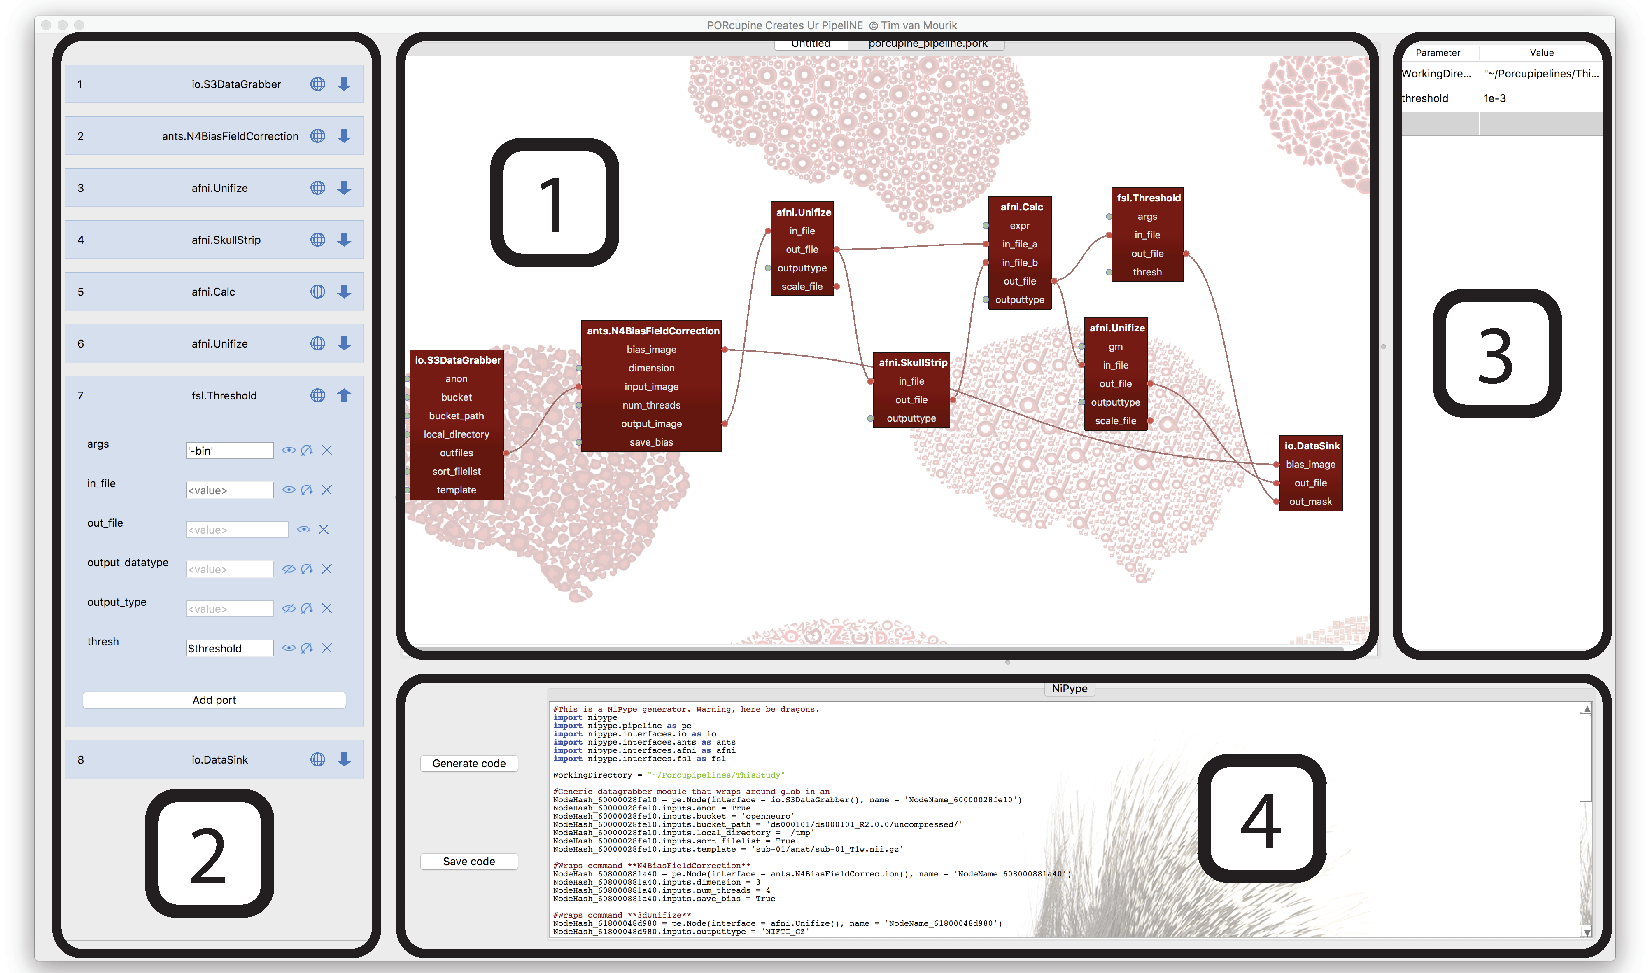
\includegraphics[width=0.9\textwidth, clip=true]{./Chapters/05_Porcupine/./Images/gui_showcase.pdf}
	\caption{A screenshot of a Porcupine workflow. The editor is divided into four panels, each of them targeted at facilitating a more understandable and reproducible analysis. The \emph{workflow editor} (1) provides a visual overview of one's analysis. The functions are all listed in the \emph{node editor} (2), where the parameters for all functions can be orderly stored. This may include links to important parameters that are listed in the \emph{parameter editor} (3), such that an overview of the main analysis settings can be easily viewed and modified. Readily executable analysis code is generated in the \emph{code window} (4)}
	\label{fig:porcupine-editor}
\end{figure}

%scope of this paper
We here focus on code generation that strictly adheres to the Nipype API \cite{Gorgolewski2011}, a Python-based MRI analysis and pipelining package. Nipype is used for its strong focus on uniformity in accessing functions, its link to most major MRI analysis tools, and its emphasis on reproducible science. Porcupine's architecture, however, is in principle agnostic with respect to the specific implementation of the underlying pipelining software. Any package with a consistent interface in the field of e.g. neuroimaging, bioengineering, or astronomy could benefit from using Porcupine's architecture.

%show by example
We first show that we can easily generate a standard fMRI analysis pipeline. After visually dragging and dropping modules, code is automatically created that is usually scripted manually instead. We then show how we facilitate loading data from an online repository, generate a readily executable fMRI pipeline, but also generate a shareable and reproducible analysis environment (using Docker), all with minimal additional effort. This allows for easily scalable analyses that \change{could}{can} be performed locally, but also on computational clusters or with cloud computing, without manual installation of different software packages. 

\subsection{Usage example}
We here show a simple example that constructs a pipeline for a single operation. In three steps, data is loaded, (minimally) processed, and the output is written to disk, as shown in Fig.~\ref{fig:porcupine-simple}. We here show an example that links to an OpenNeuro fMRI data set, but we could load any online data set that is set up according to the BIDS format \cite{Gorgolewski2016}. OpenNeuro's data sets are stored as Amazon repositories (`S3 buckets') and can be loaded by dragging the appropriate module into the workflow editor and typing the name of the bucket into the node editor. Its output can subsequently be connected to a Nipype function node, for example FSL's Brain Extraction Tool. All parameters of the function are listed and can be set in two different ways: either by dragging a link from a previous node's output port to an input port in the next node, or by typing in the parameter in the node editor. Subsequently, output can be written to disk by connecting the desired output to a Nipype DataSink node that collects and stores the data. By pressing the `Generate code` button, the code for this pipeline is automatically generated and can immediately be saved and executed in a Python shell.
\begin{figure}[!ht]
	\centering
	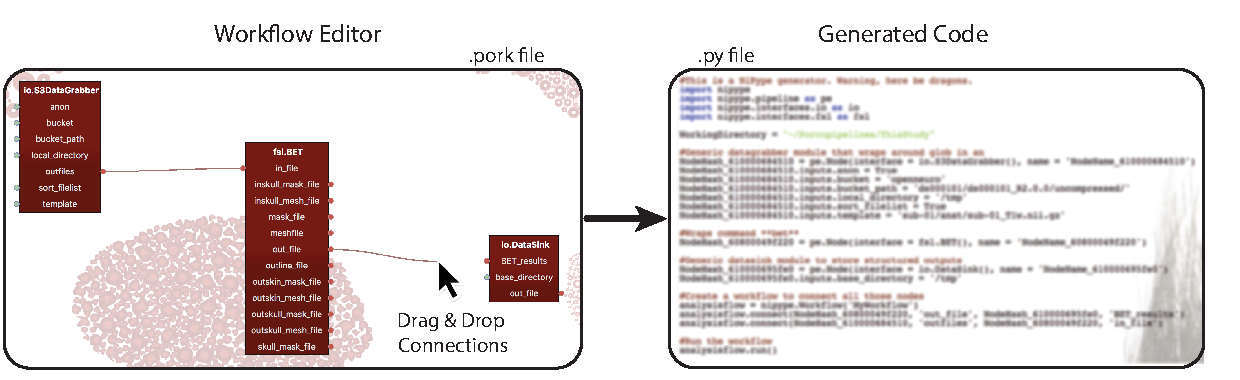
\includegraphics[width=0.9\textwidth, clip=true]{./Chapters/05_Porcupine/./Images/pork_py.pdf}
	\caption{An example of simple workflow. In three steps, this pipeline loads data, processes it, and writes it to disk. This is achieved by connecting the input and output fields from subsequent nodes in the pipeline. The constructed workflow is then transformed in readily executable (Nipype) analysis code.}
	\label{fig:porcupine-simple}
\end{figure}


\subsection{Pipeline sharing}
From a simple example that reads and writes the data, a more complicated pipeline is readily set up. More functionality, i.e. nodes, can be dragged in and connected to quickly build a custom pipeline. As it is commonplace to repeat a single analysis or function for several subjects, sessions, or other variables, every field can be flagged as an `iterator' field. This facilitates looping over variables. Once the pipeline is set up and the code is generated, Nipype offers functionality to construct a visual pipeline graph from custom python code. In Porcupine's proposed use-case, this end point of a standard Nipype pipeline represents the starting point, as shown in Fig.~\ref{fig:porcupine-advanced}. This allows the user to focus on the desired pipeline graph first, and then progress to the manual editing of the generated code.
\begin{figure}[!ht]
	\centering
	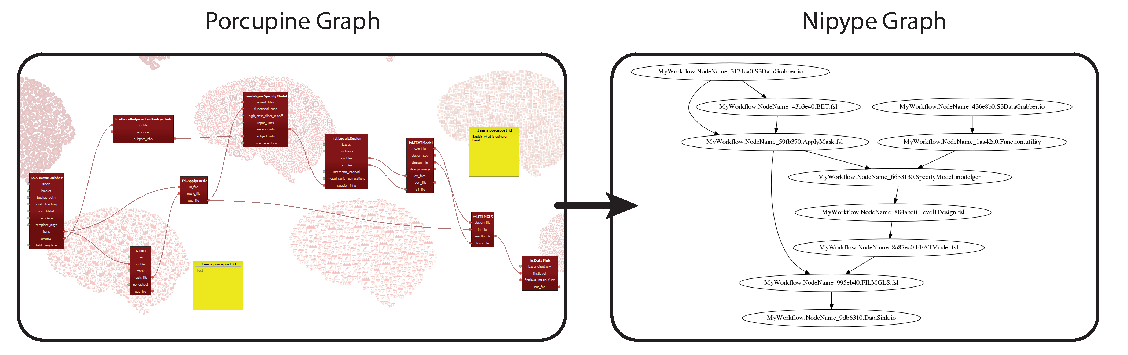
\includegraphics[width=0.9\textwidth, clip=true]{./Chapters/05_Porcupine/./Images/pork_graph.pdf}
	\caption{An example of a more complicated and realistic fMRI preprocessing pipeline. Once the code is generated, this can in turn be transformed into a Nipype graph visualisation. Whereas this is usually the end point for a pipeline in Nipype, we here propose to use a visualisation as a starting point of one's analysis.}
	\label{fig:porcupine-advanced}
\end{figure}

Not only does Porcupine provide a way of setting up a preprocessing  or analysis pipeline, we also provide a means for executing these pipelines in a reproducible environment. In addition to the Python analysis file that is generated, we create a scaffold for a Docker file. Docker (\url{https://www.docker.com}) is an open platform to easily build, run and share applications. The generated Docker file describes a minimal operating system that is required to run the analysis, based on the dependencies of the modules used in the workflow editor. With this Docker file, an image of the full analysis can be built, shared and executed. This provides a simple platform to reproduce results of one's analysis, on the same data set, or on another with only a single change in the data source module. Alternatively, one can use it as a template environment for a new follow-up analysis. As with all generated code, the Docker code is fully customisable to a researcher's need, but our suggested scaffold requires only a single manual edit to be built as a Docker image (see~\nameref{app:docker}). The Docker command will execute the pipeline: load the data from an online repository, process the data, and store only the output data to a local directory. The Docker image includes both the pipeline code and the run environment, and can be shared alongside a paper via DockerHub. The above examples (and many more) as well as extensive documentation and tutorials can be found \href{https://timvanmourik.github.io/Porcupine}{here}.

\subsection{Limitations}
Some features in Nipype have not been implemented. Notably, the JoinNode functionality is not yet accessible from the Porcupine user interface, in which the results from an upstream iterator are aggregated to a single output. Furthermore, custom extensions of Nipype functions are not automatically supported, but we do provide a script to add one's own custom module to Porcupine that would make this functionality accessible. A GUI for this is still an intended point of improvement. In general, feature requests are maintained as \add{\emph{issues} and} \emph{projects} in the \href{https://github.com/TimVanMourik/Porcupine/projects}{GitHub repository}. We encourage people to contribute new ideas or implementations for functionality in terms of modules, new toolboxes, and, most importantly, custom pipelines that can be added to the repository. Details \change{for contributing}{on how to contribute} can be found on the website.

While Porcupine in principle supports all workflow operations, a specific pipeline may well require modules that are not provided within Nipype. It is advised that the user either packages custom code for this into a new module, or manually adds it to the produced code. \change[Reviewer 2]{Porcupine itself functions only as the front-end to the Nipype back-end, but}{We furthermore stress that Porcupine is intended to function as a front-end encapsulation of NiPype, and does not implement the parsing of python files that contain pre-defined nipype pipelines. It also} does not perform type-matching on the input and output of a connection, nor does it perform syntax checking of the manually edited parameters.
\section{Design and Implementation}
Porcupine's graphical user interface was written first with a general visual programming application in mind. The initial interface to Nipype was developed at a three-day coding sprint at BrainHack 2017, Amsterdam. This kickstarted Porcupine in its current form. The source code, as well as the installer files for Windows, Mac, and Linux, are publicly available as a \href{https://github.com/TimVanMourik/Porcupine}{GitHub repository}. Porcupine is free, open source, and released under the GNU General Public License v3.0. \add[Reviewer 1]{It has static digital object identifier (DOI)} \url{doi.org/10.5281/zenodo.1146653}.

Visual programming is a generic way of programming to create a data flow or to perform an ordered task with a modular structure \cite{Myers1986}. Customarily, it allows the user to construct a Directed Acyclic Graph (DAG) \cite{Thulasiraman1992} of conceptualised operations that are subsequently interpreted or compiled as an application \cite{Myers1990}. This format is particularly useful for workflows that fit modular structures, such as most neuroimaging data analyses \cite{Rex2003}. 

\subsection{Architecture}
Not only do we intend researchers to make their analyses (re-)usable and robust, our software also adheres to all 20 simple rules that were laid out to this end \cite{List2017,Taschuk2017}. The updates as well as the releases of the source code are realised by means of a GitHub repository. Installer files are provided for all platforms and do not require administrator privilege. Users are aided in getting started quickly by extensive documentation and an example gallery.

Easy cross-platform installation or compilation was achieved by programming Porcupine as a stand-alone application in Qt Creator (\url{https://www.qt.io}) for C++. Internal file formats were standardised to JSON dictionaries, a format native to Python, Qt, and web applications. This provides a simple means to add new modules to Porcupine, without the need to write additional code. Every dictionary specifies a software package (e.g. `Nipype', `Docker', etc.) that is interpreted by Porcupine and creates code that is native to the package. A package-specific interpreter needs to be written just once, after which new modules that are included in the dictionary will be automatically available in Porcupine.

%the dictionaries
Each JSON dictionary describes a list of functions (internally referred to as 'nodes'). Each function has a name and (optionally) a category, a web url to its documentation, and a block of code. A code block specifies the software package for which the node is meant, the associated piece of code for that function and optionally an additional comment. Furthermore, a node contains any number of data/parameter ports, each of which can be input, output, or both. Optionally, additional flags can be set for ports to be visible in the editor, whether its value is editable, or whether the variable needs to be iterated over. Thus, JSON files for custom nodes can easily be created and added as a dictionary to the graphical interface. We also provide a Python script that converts a custom Python function(s) to a Nipype node dictionary.

\subsection{Extending Porcupine with new toolboxes}
Currently, Porcupine features Nipype and Docker support, but this could easily be extended to other software packages. This requires no major changes to the Porcupine source code, merely the inclusion of a single C++ class that describes the relationship between the nodes, links, and the output code. Specifically, the `CodeGenerator` class must be inherited and has access to the full workflow: the list of nodes, their parameters, and their connections. As long as all functions within an analysis toolbox can be accessed with a consistent interface, they can be represented as modules within Porcupine. Apart from Nipype, support for a laminar specific fMRI analysis toolbox in MATLAB is provided. The developers of the Fastr framework programmed initial support for their code base \cite{Achterberg2016}. Unfortunately, only few neuroimaging packages abide by this uniformity of their functions and hence many cannot be included into Porcupine.

\subsection{Relation to existing pipeline managers}
Porcupine aims to provide an extendable, transparent and flexible platform to build preprocessing and analysis pipelines. Other software packages have made similar attempts at providing visual aids to build or run pipelines. Within neuroimaging, the most notable ones are the JIST pipeline \cite{Lucas2010}, extended with CBS Tools \cite{Bazin2014} and the LONI pipeline \cite{Rex2003}. Porcupine distinguishes itself from these by not creating a run environment, but instead creating the analysis code for the researcher. This retains the possibility of immediately running the code through a Python interpreter, but also creates more flexibility, as researchers can modify and adjust the script according to their needs.\remove[Reviewer 3]{Additionally, as the functions link to existing Nipype interfaces, error reporting is more transparent such that problems can more easily be resolved.} Lastly, our open-source framework is set up to be extendable with new modules within existing frameworks, as well as with completely new frameworks. This provides a future-proof set-up for current and future analysis tools in neuroimaging and perhaps other disciplines.

\section{Availability and Future Directions}
We have presented a new tool to visually construct an analysis pipeline. Subsequently, Porcupine automatically generates the analysis code, and provides a way of running and sharing such analyses. We see this as an important tool and a stepping stone on the path to doing more reproducible and open science. Additionally, this gives researchers a better oversight of their analysis pipeline, allowing for greater ease of developing, understanding, and communicating complex analyses.

Porcupine provides two independent functionalities that dovetail to allow users to more easily take part in reproducible neuroimaging research. They are (1) a graphical user interface for the visual design of analysis pipelines and (2) a framework for the automated creation of docker images to execute and share the designed analysis. 

We anticipate that the ability to design processing pipelines visually instead of programmatically \change{cuts}{will cut} the novice user's learning phase by a considerable amount of time by facilitating understanding and development. The ease of use of a Graphical User Interface (GUI) implementation extends and complements Nipype's flexibility. Thus, it invites researchers to mix and match different tools, and adhere less stringently to the exclusive use of the tools of any given toolbox ecosystem. This flexibility enhances the possible sophistication of processing pipelines, and could for instance be helpful in cross-modal research or multi-site research. Additionally, it may nudge method developers to write new tools in a way that easily integrates with the Nipype and Porcupine structure.

The emphasis that Porcupine puts on visual development of analyses makes it easier to communicate a methods section visually rather than in writing. We foresee that researchers may prefer explicity sharing the created .pork files and the Nipype pipelines that are created from them, instead of solely relying on written descriptions of their methods. Yet another use case for Porcupine is the easy definition of proposed processing workflows for preregistered studies.

Importantly, Porcupine attempts to reduce the steepness of the learning curve that is inherent to the use of complex analysis, by providing a more structured and systematic approach to pipeline creation. It separates the skill of building a conceptual analysis pipeline from the skill of coding this in the appropriate programming language. This places Porcupine in a position to aid in the education of novice neuroimaging researchers, as it allows them to focus on the logic of their processing instead of the creation of the code for the processing - greatly improving and accelerating their understanding of the different steps involved in the preprocessing of neuroimaging data. At the same time, it allows more experienced researchers to spend more time on \change[Reviewer 2]{theconceptual}{the conceptual} side than on implementational side.

Having allowed for the visual design of a pipeline for the preprocessing or analysis of a neuroimaging dataset, the reproducible execution of this pipeline is another step that Porcupine facilitates. By flexibly creating a Docker image tailored to the different preprocessing steps defined visually in the GUI, Porcupine allows the user to share not only the definition of the pipeline but also its execution environment. This step removes the overhead of having to manually install the desired operating system with the matching distribution of MRI analysis software. This final step greatly facilitates the reproducibility of reported results, and is part of a general evolution of the field towards easily shareable and repeatable analyses. 

The generated Docker image can be made High Performance Computing aware \remove{with singularity} by means of dedicated tools such as \href{https://github.com/singularityware/docker2singularity}{docker2singularity}. Alternatively, with only trivial additions to the Dockerfile, it can be transformed into a BIDS app \cite{Gorgolewski2017}. A detailed explanation for doing this can be found on our \href{https://timvanmourik.github.io/Porcupine/documentation/advanced/make-a-bids-app}{website}. An automatic and direct way of creating \add{this} has not yet been implemented. Additionally, integrating support for standardised workflow file formats, such as the Common Workflow Language \cite{Amstutz2016} could further add to Porcupine's aim of reproducibility. Another point of improvement is a functionality to embed pipelines within pipelines. Currently, a complicated pipeline\remove[Reviewer 2]{s} does full justice to the term `spaghetti code', and the number of nodes and links may easily compromise the visual aid in understanding; the very purpose for which Porcupine was created. This may easily be solved by compartmentalising pipelines into logical units by providing an embedded structure.

We intend Porcupine to be a strong aid for doing better, more reproducible and shareable science. By bridging the gap between a conceptual and implementational level of the analysis, we give scientists a better oversight of their pipeline and aid them in developing and communicating their work. We provide extensive and intuitive documentation and a wide range of examples to give users a frictionless start to use Porcupine. We look forward to adding more functionality and\change{support for}{supporting} more toolboxes in the near future.

\section{Supporting information}
\paragraph*{S1 Docker files}
\label{app:docker}
Porcupine provides a Docker image that creates the necessary run time environment for a pipeline that is constructed in the workflow editor. As with all generated code, the Docker code is fully customisable to a researcher's need, but our suggested scaffold requires only a single manual edit to be built as a Docker image. A Docker script can only refer to online or on-disk resources, so the pipeline file needs to be saved manually and added to the Docker file:
\begin{lstlisting}
ADD /path/to/pipeline/script.py /somewhere/porcupipeline.py
CMD ["python", "/somewhere/porcupipeline.py"]
\end{lstlisting}
Once this line is added, the docker image can be built:
\begin{lstlisting}
$ docker build -t mydockerimage -f Dockerfile
\end{lstlisting}
The output from the executed pipeline can be written to a local directory on a researcher's computer (`/my/local/directory') by mounting it to the docker output directory (`/data') with the `-v' option and running the image as if it were a standalone application.
\begin{lstlisting}
$ docker run -v /my/local/directory:/data mydockerimage
\end{lstlisting}
This Docker command will execute the pipeline: load the data from an online repository, process the data, and store only the output data to a local directory. A fully worked out example with detailed explanation can be found \href{https://timvanmourik.github.io/Porcupine/documentation/basics/building-dockerfiles}{here}.
\section{Acknowledgements}
We would like to  thank the organisation of BrainHack Global and BrainHack Amsterdam, specifically Pierre-Louis Bazin, for organising the platform that kickstarted Porcupine in its current form. Tim van Mourik acknowledges support by Spinoza grant SPI 40-118.
\section{Author contributions}
TvM wrote the Porcupine C++ software. TvM, LS, and TK designed the interface to Nipype. LS and TvM built the website. LS wrote the examples and the majority of documentation. TvM, TK, LS, and DGN wrote the paper.

 \afterpage{\blankpage}
 
\chapter{Summary and Discussion}
\chaptermark{Discussion}
\label{ch:discussion}

For long the nature of the processing undertaken by the cortical layers has been recognised as a mystery that needs to be resolved to better understand the computations being performed by our brains \cite{Miller2001}. The most realistic method to date of studying this in living human subjects is with functional MRI, as it it very precise and non invasive. But many challenges in spatial and temporal resolution, resolution, interpretation, and all sorts of noise have to be overcome before this can be easily used to solve neuropsychological problems. The objective of this thesis was to pave the way for doing more routine laminar fMRI analysis. Indeed we made significant steps towards this end. 
We have developed several new methods that solve major problems in laminar analysis, we conducted a full layer specific analysis, and took explicit care to make everything along the way reproducible and reusable. %% <-- unpack

\section*{Chapter 2: Recursive Boundary Registration}
First, we addressed the problem of local distortions that are often present in Echo Planar Images (EPI). Due to inhomogeneities in the main magnetic field, spins in some areas rotate a bit faster or slower than others. Effectively, this causes small shifts of parts of the image with respect to the true position. Thus, even though the true locations of the layers are known, the distortions may easily be larger than the thickness of the layers. Without correcting this effect it is hopeless to get out any reliable layer signal. So that is what we set out to do in Chapter 2.

Geometry transformation from one volume to the other (coregistration) has been very succesful for linear transformations and is used routinely in fMRI analysis. Even on volumes with low resolution, low contrast, or few slices, it may work well \cite{Greve201}, but not for non-linear transformations. Such transformations require a high number of degrees of freedom because of the many parameters that need to be estimated. This leaves much more room for error and therefore usually only works on high contrast data sets. It is used routinely for transforming single subject anatomical space to a template space with the same contrast. However, existing techniques are not powerful enough to undistort low contrast EPI images. We therefore invented a new technique for this, Recursive Boundary Registration. By recursively applying linear transformations on diminishing spatial scales, we effectively compute a non linear registration. In order to guarantee smoothness over all transformations, it is combined with a control point lattice that regulates the transformations. Explicitly taking the geometry of the volume into account as a type of prior knowledge is a novel way to approach non linear registrations.

We tested RBR on two different types of data. First, in order to establish a gold standard, we distorted a FLASH image that is typically without distortion. Because we did this in a controlled manner, we could easily compare the performance of RBR to our ground truth and verify the quality of the registration. We thus proceeded to EPI data set of 11 subjects that had real distortions. As the true size of the distortions was unknown there cannot be an absolute quality metric for the registration. Instead, by adding different levels of noise we showed that there is a clear SNR dependance in the displacement that decreases towards the no-noise condition. Additionally, we provide an abundance of graphical evidence to illustrate the performance of RBR.

The power of the method lies in the fact that it makes explicit use of the gyrification of the brain and the specific geometry of an individual brain. It can therefore get away with little contrast and still produce an accurate registration while preserving the topology of the original. Because of the large number of parameters that needs to be estimated we built in a variety of robustness assurances. Despite the overall improved registration, it is still important to carefully inspect the quality of the registration to verify the required submillimetre accuracy. All in all, this proved to be a valuable tool for preparing Gradient Echo images for subsequent analyses and we use it in our experimental study in Chapter 4. It is now an integral part of the fMRI analysis toolbox for laminar fMRI, \url{https://github.com/TimVanMourik/OpenFmriAnalysis}.

An helpful realisation in developing this method was a more conceptual look on the problem. The problem of coregistration can be classified along two main axes: the type of image contrast can be different or the same, and the required transformation can be linear or non linear. The easiest scenario is to find a linear transformation for a volume with similar contrast. The problem becomes harder when the volume has a different contrast, as the mapping of intensity values from one volume to the next is unknown. If instead the contrast is the same but the required transformation is non linear, it is still solvable to a good approximation \cite{Collins1995}. However, when the contrast is different \emph{and} the registration should be non-linear the, the degrees of freedom of the problem increases drastically, and is not easily estimated anymore. Combine this with the low contrast-to-noise ratio of fMRI data and it is clear that this is a hopeless endeavour with standard volume-to-volume registration. The trick to solve this conundrum is to introduce more prior knowledge to the equation. In this case, we chose to use the geometric information of the cortex and its many gyri and sulci to more accurately estimate a non linear cross-modal registration. This does the trick on a single subject level, but by introducing prior knowledge, we restricted the use cases. Where the previous non-linear transforms could also compute subject-to-template registration, we lost this ability by strictly enforcing equal geometry across volumes. As a general notion, algorithms can become more powerful when they are more specialised. Usually this requires a specific type of prior knowledge in the data that is quantified and optimised.

\section*{Chapter 3: Spatial GLM for laminar fMRI}
Once the geometry of our cortical surfaces is properly aligned with our functional data, there is a next problem: how can the laminar signal be extracted from the MRI volume? There are several intuitive ways. A volume could simply be interpolated at the approximate location of the layers, or classify voxels to be part of it most likely layer. However, it is clear that this inherently smears out the laminar signal to some extent. In Chapter 3 we set out to quantify this signal leakage and to present a new method to reduces it and to more cleanly separate the laminar signal.

We started out with the notion that all voxels are a mixture of a variety of layers. If this mixture could be accurately modeled it could theoretically also be inverted and solved for the layer intensity values by means of the framework of the General Linear Model (GLM). To achieve this, we first set up a mathematical framework to accurately model the layer distribution and subsequently estimate the layer signal intensity. 

Our cortex model incorporates information about the precise location, curvature and thickness of the cortex to model the 



We previously mentioned that methods can become more powerful when they use types of prior knowledge inherent to the data. We here find that this is true, but might come at the cost of a la

The prior knowledge 


Due to the many factors that could play a role in the 
The combinatoric explosion of the many dimensions

\section*{Chapter 4: Layer Specificity in Visual Attention}


"In addition, excitatory neurons may quickly redistribute input from the thalamus by means of their local axonal collaterals, 
so that cortical activity nearly instantaneously spreads over several layers and columns to mediate perception of sensory stimuli (Reyes-Puerta et al., 2015)"

publication bias 
null result


\section*{Chapter 5: Pipelines for fMRI with Porcupine}






\linespread{1.5}
\newpage
 \afterpage{\blankpage}
 \chapter{Appendix}
\chaptermark{Appendix}
\thispagestyle{empty}
\bibliographystyle{abbrv}
\renewcommand{\bibsection}{\section{Bibliography}}
\bibliography{Bibliography/Bibliography}

\newpage
\section{Nederlandse samenvatting}
In dit proefschrift zoomen we zo ver mogelijk in op het brein, en proberen we een glimp op te vangen van de processen die daar plaatsvinden. Door iedere paar seconden een driedimensionale afbeelding te maken van het brein kunnen we een indruk krijgen wat er zich daar afspeelt. Op een grove schaal kunnen we zien welke breingebieden actief worden bij verschillende taken: als het licht aangaat, wordt de achterkant van je brein actief (de \emph{visuele cortex}), en voornamelijk de linker zijkant van het brein (je taalcentrum) wordt actief als je deze tekst leest. Maar wat betekent het dat die gebieden actief worden? Wat doen ze dan precies? Op een MRI-scanner kunnen we voornamelijk zien dat gebieden meer of minder zuurstof verbruiken. Dat vertelt echter niet zo gek veel over het proces wat zich daar afspeelt. Om daar iets beter achter te komen, moeten we nog verder kijken. Dankzij anatomische ontledingen van het brein weten we dat de buitenste schil van het brein, de grijze stof, uit verschillende laagjes bestaat. Sommige lagen ontvangen informatie en sommige lagen sturen het door naar de andere breingebieden. Het doel van dit proefschrift is de functie van verschillende lagen te laten zien op basis van MRI-scans.

Dat is echter niet makkelijk: de laagjes zijn zo klein dat de resolutie van de MRI-scanner maar ternauwernood goed genoeg is. En daar komt nog bij dat de plaatjes die uit een MRI-scanner komen zelf ook licht verschoven zijn. Vervolgens moet je erachter zien te komen hoe, in een kronkelend brein, de laagjes precies verdeeld zijn over alle volume-pixels (voxels) van het driedimensionale plaatje. En verder wilden we dit niet gewoon \'e\'en keer uitvoeren, maar zorgen dat iedereen dit type onderzoek voortaan ook kan doen.

% hoofdstuk 2
In \textbf{hoofdstuk 2} zijn we begonnen met het eerste probleem: binnen de afbeeldingen die uit de MRI-scanner komen, liggen de verschillende lagen niet exact op de goede plek. Dit heeft te maken met de manier waarop een MRI-scanner werkt: in het midden van scanner wordt een groot magneetveld gecre\"eerd wat cruciaal is voor het maken van scans. Echter, als het magneetveld niet exact homogeen is, vertaalt dit zich in de scan als kleine (lokale) verplaatsingen. Omdat het nou juist cruciaal is tot op het kleinste niveau op de goede plek te meten als je de verschillende lagen wil meten, is dit een groot probleem. Daarom hebben we een methode bedacht om de scan `recht te trekken' en weer terug op de goede plek te leggen. Op basis van beeldanalyse kijken we heel precies waar de grenzen van de witte en grijze stof zitten, ten opzichte van een niet verplaatste referentie scan. We laten vervolgens op verschillende data sets zien dat de methode daadwerkelijk een veel preciezer beeld geeft over de locatie van de verschillende lagen. 

% hoofdstuk 3
Hiermee is de locatie van de lagen met hoge precisie bekend. Het hele hersenoppervlak ligt echter nog steeds gekronkeld in het volume en de verschillende lagen zijn zo klein dat ze nog niet duidelijk te zien zijn. In \textbf{hoofdstuk 3} beschrijven we een nieuwe methode op basis waarvan de signalen uit verschillende lagen beter geschat kunnen worden. Dit doen we door middel van een wiskundig model dat beschrijft hoe de laagjes verdeeld zijn over het volume. Aan de hand van dit model kunnen we preciezer dan voorheen de signalen uit de lagen halen. Op basis van drie verschillende datasets laten we zien hoe deze nieuwe methode presteert. In een simulatie van een MRI-volume blijkt het veel beter te werken dan bestaande methode. Dit is echter niet zo duidelijk in data van echte scans. De reden hiervoor is dat onze methode op goede data inderdaad een betere schatting kan maken, maar wel gevoeliger is voor ruis in de data. Dat maakt het moeilijk goed zicht te krijgen op het verschil tussen de methodes op standaard MRI-scans.

% hoofdstuk 4
Na deze twee methodologische studies om de weg vrij te maken voor laag-specifieke analyse, hebben we in \textbf{hoofdstuk 4} geprobeerd uit te zoeken of de lagen inderdaad verschillende activatie tonen bij verschillende processen. Hiervoor hebben we een aandachtstaak gebruikt. We vroegen mensen hun aandacht links of rechts te focussen en af en toe verscheen er een stimulus (een zwart-wit gestreept plaatje) op het scherm. Zo wilden we onderzoeken of het effect van aandacht in andere lagen te zien valt dan het effect van het zien van een stimulus. Op brein niveau was er wel degelijk een effect te merken, maar op laagniveau zagen we geen verschil. Dit is dus een nul-resultaat met betrekking tot de signalen uit de verschillende lagen. Het is moeilijk te zeggen wat hier precies de reden van is: of het effect niet bestaat, of het effect niet sterk genoeg was, of dat de methodes niet goed genoeg waren om het eruit te halen (of een combinatie van factoren).

% hoofdstuk 5
\textbf{Hoofdstuk 5} gaat over een applicatie die we ontwikkeld hebben om het makkelijker te maken om MRI data te analyseren, Porcupine. Analyses bestaan doorgaans uit lange scripts die een aaneenschakeling beschrijven van verschillende bewerkingen die uitgevoerd moeten worden op de gemeten data. Onderzoekers schrijven deze analyse code vaak zelf, maar deze scripts zijn vaak moeilijk te interpreteren. In plaats hiervan kan een analyse in Porcupine visueel geprogrammeerd worden door blokjes aan elkaar te verbinden. Dit representeert de volgorde van de analysestappen en laat zo op een grafische manier zien hoe de `workflow' eruit ziet. Porcupine genereert vervolgens de analyse code die direct uitgevoerd kan worden. Omdat dit een inzichtelijke weergave biedt die makkelijker deelbaar is en makkelijker valt aan te passen dan huidige analyse scripts, zorgt dit voor een reproduceerbaardere wetenschap.

% Concluding remarks
Hiermee maakt het werk in dit proefschrift de weg vrij om de lagen van de cortex meer routinematig te analyseren. Alhoewel we in dit onderzoek geen effecten gevonden hebben, lijken andere studies (die dezelfde methodes hebben gebruikt) wel resultaten op te leveren. Het is dus nog onduidelijk wat voor informatie er precies te vinden is als we met die precisie in het brein proberen te kijken. Laag-specifieke brein analyse in functionele MRI staat hiermee dus nog in de kinderschoenen, en onze methodologische ontwikkelingen staan hieraan ten grondslag.





\newpage
\section{Biography}
\addcontentsline{toc}{chapter}{Biography}
Tim van Mourik was born on September 27th 1990 in Leiden, the Netherlands. After graduating from the Stedelijk Gymnasium Leiden, he went on to pursue a Bachelor's degree in the exact sciences at the Roosevelt Academy (currently: University College Roosevelt). After this, he enrolled in the Master Computer Animation and Visual Effects at Bournemouth University. Over the course of this program, he started to develop an interest in medical image processing and completed the program with an internship at the Donders Centre for Cognitive Neuroimaging under the supervision of prof. David Norris. As MRI scanners operate on physical and mathematical principles, subsequently producing three-dimensional images, this perfectly combined Tim's expertises and interests. He continued to work as a research assistant at the Donders Institute where he was initiated in the world of neuroimaging and laminar analysis. In February 2014, he started a four-year PhD project to investigate and better understand the cortical layers of the brain. During this time he developed methods for better analysing laminar fMRI data and under the supervision of Dr. Janneke Jehee, he conducted a study on the layer specificity of spatial attention. All tools, code, and data for his published work is openly available, as Tim is a strong proponent of open science, data and code sharing, and open source development. In this spirit, he programmed worfklow software, Porcupine, that automatically and more transparently creates analysis code. He is currently contuining this line of work by creating an online platform for easier data sharing, GiraffeTools. It is unknown where he acquired his peculiar taste for silly acronyms. For these efforts towards open science he was elected to be the chair of the Open Science Room at OHBM 2019, Rome. 

\newpage
\section{Author publications}

\subsection{Published papers}

\hangindent=2em
\noindent
% Author
\textsc{\textbf{T.~van Mourik}, L.~Snoek, T.~Knapen, and D.~Norris.} 
% Year
(2018).
% Title
Porcupine: a visual pipeline tool for neuroimaging analysis.
% Journal
\emph{PLoS computational biology.}


\hangindent=2em
\noindent
% Author
\textsc{S.~Lawrence, \textbf{T.~van Mourik}, P.~J. Koopmans, D.~Norris, and F.~de~Lange.} 
% Year
(2018).
% Title
Laminar Organization of Working Memory Signals in Human Visual Cortex. 
% Journal
\emph{Current Biology, in press.}


\hangindent=2em
\noindent
% Author
\textsc{N.~Z.~Bielczyk, S.~Uithol, \textbf{T.~van Mourik}, P.~Anderson, J.~C.~Glennon, and J.~K.~Buitelaar} 
% Year
(2018).
% Title
Disentangling causal webs in the brain using functional Magnetic Resonance Imaging: A review of current approaches.
% Journal
\emph{Network Neuroscience.}


\hangindent=2em
\noindent
% Author
\textsc{R.~Scheeringa, P.~J.~Koopmans, \textbf{T.~van Mourik}, D.~Norris, and Jensen.} 
% Year
(2016).
% Title
The relationship between oscillatory {EEG} activity and the laminar-specific bold signal.
% Journal
\emph{PNAS.}


\hangindent=2em
\noindent
% Author
\textsc{P.~Kok, L.~Bains, \textbf{T.~van Mourik}, D.~Norris, and F.~de~Lange.} 
% Year
(2016).
% Title
Selective activation of the deep layers of the human primary visual	cortex by top-down feedback.
% Journal
\emph{Current Biology.}


\hangindent=2em
\noindent
% Author
\textsc{M.~Kleinnijenhuis, \textbf{T.~van Mourik}, D.~G. Norris, D.~J. Ruiter, A.-M. van	Cappellen~van Walsum, and M.~Barth.} 
% Year
(2015).
% Title
Diffusion tensor characteristics of gyrencephaly using high	resolution diffusion {MRI} in vivo at 7{T}.
% Journal
\emph{NeuroImage.}



\subsection{Publications in preparation}

\hangindent=2em
\noindent
% Author
\textsc{\textbf{T.~van Mourik}, P.~J. Koopmans, L.~J. Bains, D.~G. Norris, and J.~F. Jehee.} 
% Title
Investigation of layer specific bold during visual attention in the human visual cortex.
% Journal
\emph{In preparation.}


\hangindent=2em
\noindent
% Author
\textsc{\textbf{T.~van Mourik}, P.~J. Koopmans, L.~J. Bains, and D.~G. Norris.} 
% Title
Improved cortical boundary registration for locally distorted fMRI scans.
% Journal
\emph{Submitted, Preprint on bioRxiv.}


\hangindent=2em
\noindent
% Author
\textsc{\textbf{T.~van Mourik}, J.~P.~J.~M.~ van der Eerden, P-L.~Bazin, D.~G. Norris.} 
% Year
(2018).
% Title
Laminar signal extraction over extended cortical areas by means of a spatial GLM.
% Journal
\emph{Submitted, Preprint on bioRxiv.}


\hangindent=2em
\noindent
% Author
\textsc{F.~Molaei-Vaneghi, N.~Zaretskaya, \textbf{T.~van Mourik}, J.~Bause, K.~Scheffler, and A.~Bartels.} 
% Title
9.4 T Human fMRI Study Reveals that Real World Motion Perception Does Not Involve Laminar Organization in V1 and V5/MT.
% Journal
\emph{Submitted.}


\hangindent=2em
\noindent
% Author
\textsc{S.~H.~P.~Collin, P.~van den Broek, \textbf{T.~van Mourik}, P.~Desain, C.~F.~Doeller.}
% Title
Creating an artificial memory context alters associative memory formation.
% Journal
\emph{In preparation.}

\newpage
\section{Acknowledgements}

Over the six years that I spent working at the Donders Institute I have met so many people without whom this thesis would not be what it is today. I cannot do justice to of you but I will at least try for a small subset.

%%%%%% David
First, I would like to thank my supervisor, promotor David Norris. When I came in as a student of the exact sciences I preferred to put \emph{quod erat demonstrandum} at the end of every paragraph. You taught me a lot about the scientific method in neuroscience, bigger pictures and the gran(d/t) scheme of things, the politics of laminar analysis, and much more. Our Bert and Ernie roles that we took on in meetings for me lead to more out-of-the-box thinking and I hope that I managed to form them into pragmatic and realistic solutions. I am thankful for the way in which you stay close to the real science and the amount of dedication and personal attention you give to your students, while still having them to express their autonomy to become an independent researcher.

%%%%%% Janneke
I would especially like to thank my co-promotor Janneke Jehee. Visual computation, so I found out, has nothing to do with visual effects, and also not so much with computers. My very first email to the Donders Institute was to inquire about a position in your lab. But you kindly explained that the computations of the visual cortex might not suit my interest or skillset and referred me to the head of the MR physics lab. It was years later that our paths crossed again when you took me up in your lab when I wanted to study layers in the visual cortex. I am very grateful for the time and dedication with which you helped me conduct this study from beginning to (pending) end. I truly admire your dedication, resilience, and extreme precision with words, analysis, and way of doing science. The time that I spent in your lab has hooked me to the workings of the visual cortex, but it has certainly broadened my horizon, made me a better scientist, for which I am very grateful.

%%%%%% The FAD
When I started as a research assistant, there was still a dedicated culture of Friday Afternoon Drinks. From the very first week on, this made me feel welcome at the Donders and familiarised me in no time with all restaurants in Nijmegen and Romagna. And fortunately it was not all too often that this resulted in knife fights over a glass of white wine. Although the old gang has left the building (save some Donders dinosaurs), but the FAD still remains, and I would like to thank everybody with whom I have conversations and discussion to brighten up my Friday afternoon.

%%%%%% The Kitchen
Thanks to everybody in the kitchen, the old kitchen and the new canteen, for a countless number of lunches, coffees, random cake days (and those rare random suit-up days), and much more. Whether the topic of the day was general linear models, the state of science, of the world, of Brexit, or just pink elephants and the order of the day, I appreciated the diverse and stimulating environment. Over the last six years the Donders grew out from a village to a city, with all its infrastructural perks, but without the `market square' like atmosphere in the kitchen. ``Having only a single, slow coddee machine in a research institute is an underappreciated method for enhancing interdisciplinary collaboration'' (Mostert 2016).

%%%%%% Lab group
I would like to thank my lab group for the feedback on layers and porcupines, for sharing frustrations over rejection in the info-meeting, and for the historical geo-political discussion in the group lunches.

%%%%%% Office mates
Thanks to all office mates that I had over the years. For the company, the \emph{boekje-bijna-klaar?} encouragements, sharing in the MATLAB frustrations, the Armin moments on Friday afternoon (before the FAD of course), and much more. 
 
%%%%%% Admin
The backbone of the Donders is formed, of course, by Tildie, Ayse and the administration, Marek and the minions, and `koning-van-de-kelder' Paul. Thank you for all the help and support, and making everything run smoothly. We all know that the Donders would collapse without you. 

%%%%%% Vierkant
There is always one special week per year reserved for Vierkant, the maths puzzle camp. Thanks to all Vierkanters for this exciting and stimulating week, for the random sketches, for each one of you to bring your own kind of crazyness along. 

%%%%%% Paranymphs & family 
Thanks to my dear paranymphs, Tom, Jelle, and Annelies, for all the support along the way. Not just for the home stretch, but primarily in all the preceding years. You have been a sounding board for many a wonky idea that eventually made it to this thesis. A special thanks to my family, who may not always have understood what I have been doing all these years, but still unconditionally supported doing it.

%%%%%% Tineke
Dear Tineke, my Queen of Hearts, occupational panda and occasional sloth. Acronym expert, kindest supporter, and toughest critic. It is quite unclear where we will end up next, but it will be somewhere together. 





\newpage

\section{Donders Graduate School for Cognitive Neuroscience}

For a successful research Institute, it is vital to train the next generation of young scientists. To achieve this goal, the Donders Institute for Brain, Cognition and Behaviour established the Donders Graduate School for Cognitive Neuroscience (DGCN), which was officially recognised as a national graduate school in 2009. The Graduate School covers training at both Master's and PhD level and provides an excellent educational context fully aligned with the research programme of the Donders Institute.

The school successfully attracts highly talented national and international students in biology, physics, psycholinguistics, psychology, behavioral science, medicine and related disciplines. Selective admission and assessment centers guarantee the enrolment of the best and most motivated students.

The DGCN tracks the career of PhD graduates carefully. More than 50\% of PhD alumni show a continuation in academia with postdoc positions at top institutes worldwide, e.g. Stanford University, University of Oxford, University of Cambridge, UCL London, MPI Leipzig, Hanyang University in South Korea, NTNU Norway, University of Illinois, North Western University, Northeastern University in Boston, ETH Z\"urich, University of Vienna etc. Positions outside academia spread among the following sectors: specialists in a medical environment, mainly in genetics, geriatrics, psychiatry and neurology. Specialists in a psychological environment, e.g. as specialist in neuropsychology, psychological diagnostics or therapy. Positions in higher education as coordinators or lecturers. A smaller percentage enters business as research consultants, analysts or head of research and development. Fewer graduates stay in a research environment as lab coordinators, technical support or policy advisors. Upcoming possibilities are positions in the IT sector and management position in pharmaceutical industry. In general, the PhDs graduates almost invariably continue with high-quality positions that play an important role in our knowledge economy.

For more information on the DGCN as well as past and upcoming defenses please visit: 

\url{https://www.ru.nl/donders/graduate-school/phd}




 \afterpage{\blankpage}

\end{document}